%%%%%%%%%%%%%%%%%%%%%%%%%%%%%%%%%%%%%%%%%%%%%%%%%%%%%%%%%%%%%%%%%%%%%%%%%%%%%%%%
%%%%%%%%%%%%%%%%%%   Vorlage für eine Abschlussarbeit   %%%%%%%%%%%%%%%%%%%%%%%%
%%%%%%%%%%%%%%%%%%%%%%%%%%%%%%%%%%%%%%%%%%%%%%%%%%%%%%%%%%%%%%%%%%%%%%%%%%%%%%%%

% Erstellt von Maximilian Nöthe, <maximilian.noethe@tu-dortmund.de>
% ausgelegt für lualatex und Biblatex mit biber

% Kompilieren mit
% latexmk --lualatex --output-directory=build thesis.tex
% oder einfach mit:
% make

\documentclass[
  tucolor,       % remove for less green,
  BCOR=12mm,     % 12mm binding corrections, adjust to fit your binding
  parskip=half,  % new paragraphs start with half line vertical space
  open=any,      % chapters start on both odd and even pages
  cleardoublepage=plain,  % no header/footer on blank pages
]{tudothesis}


% Warning, if another latex run is needed
\usepackage[aux]{rerunfilecheck}

% just list chapters and sections in the toc, not subsections or smaller
\setcounter{tocdepth}{1}

%------------------------------------------------------------------------------
%------------------------------ Fonts, Unicode, Language ----------------------
%------------------------------------------------------------------------------
\usepackage{fontspec}
\defaultfontfeatures{Ligatures=TeX}  % -- becomes en-dash etc.

% english language
\usepackage{polyglossia}
\setdefaultlanguage{english}

% for english abstract and english titles in the toc
\setotherlanguages{english}

% intelligent quotation marks, language and nesting sensitive
\usepackage[autostyle]{csquotes}

% microtypographical features, makes the text look nicer on the small scale
\usepackage{microtype}

%------------------------------------------------------------------------------
%------------------------ Math Packages and settings --------------------------
%------------------------------------------------------------------------------

\usepackage{amsmath}
\usepackage{amssymb}
\usepackage{mathtools}

% Enable Unicode-Math and follow the ISO-Standards for typesetting math
\usepackage[
  math-style=ISO,
  bold-style=ISO,
  sans-style=italic,
  nabla=upright,
  partial=upright,
]{unicode-math}
\setmathfont{Latin Modern Math}

% nice, small fracs for the text with \sfrac{}{}
\usepackage{xfrac}


%------------------------------------------------------------------------------
%---------------------------- Numbers and Units -------------------------------
%------------------------------------------------------------------------------

\usepackage[
  locale=UK,
  separate-uncertainty=true,
  per-mode=symbol-or-fraction,
]{siunitx}
\sisetup{math-micro=\text{µ},text-micro=µ}

%------------------------------------------------------------------------------
%-------------------------------- tables  -------------------------------------
%------------------------------------------------------------------------------

\usepackage{booktabs}       % \toprule, \midrule, \bottomrule, etc

%------------------------------------------------------------------------------
%-------------------------------- graphics -------------------------------------
%------------------------------------------------------------------------------

\usepackage{graphicx}
\usepackage{draftfigure}
% currently broken
% \usepackage{grffile}

% allow figures to be placed in the running text by default:
\usepackage{scrhack}
\usepackage{float}
\floatplacement{figure}{htbp}
\floatplacement{table}{htbp}

% keep figures and tables in the section
\usepackage[section, below]{placeins}

% allows to include PDFs as full pages
\usepackage{pdfpages}

% Set the PDF Version of this document to 1.7 (1.4 is the current default)
% This is needed so that PDFs with Version >1.5 can be included
\pdfvariable minorversion=7

%------------------------------------------------------------------------------
%---------------------- customize list environments ---------------------------
%------------------------------------------------------------------------------

\usepackage{enumitem}

%------------------------------------------------------------------------------
%------------------------------ Bibliographie ---------------------------------
%------------------------------------------------------------------------------

\usepackage[
  backend=biber,   % use modern biber backend
  sorting=none,    % references are in appearance order
  autolang=hyphen, % load hyphenation rules for if language of bibentry is not
                   % english, has to be loaded with \setotherlanguages
                   % in the references.bib use langid={en} for english sources
]{biblatex}
\addbibresource{references.bib}  % the bib file to use
\DefineBibliographyStrings{english}{andothers = {{et\,al\adddot}}}  % replace u.a. with et al.


% Last packages, do not change order or insert new packages after these ones
\usepackage[pdfusetitle, unicode, linkbordercolor=tugreen, citebordercolor=tugreen]{hyperref}
\usepackage{bookmark}
\usepackage[shortcuts]{extdash}

%------------------------------------------------------------------------------
%-------------------------   Some commands ------------------------------------
%------------------------------------------------------------------------------

% tiks ticks ist kein zeichenprogramm :)
\usepackage{tikz}
\usetikzlibrary{calc}
\usetikzlibrary{arrows,patterns}
\usetikzlibrary{plotmarks}
\usetikzlibrary{decorations.pathmorphing}

\tikzset{snake it/.style={decorate, decoration=snake}}

\usepackage{pgfplots}
\pgfmathdeclarefunction{gauss}{3}{%
  \pgfmathparse{#3*1/(#2*sqrt(2*pi))*exp(-((x-#1)^2)/(2*#2^2))}%
}

% some math stuff to make things easier, hate the left right stuff....
\newcommand{\CL}{\ensuremath{\mathcal{L}}}
\newcommand{\CS}{\ensuremath{\mathcal{S}}}
\newcommand{\CB}{\ensuremath{\mathcal{B}}}
\newcommand{\CP}{\ensuremath{\mathcal{P}}}
\newcommand{\Vx}{\ensuremath{\vec{x}}}
\newcommand{\Vmu}{\ensuremath{\vec{\mu}}}

\newcommand{\Gp}[1]{\left( #1 \right)}
\newcommand{\Gb}[1]{\left[ #1 \right]}
\newcommand{\GB}[1]{\left\{ #1 \right\}}

%------------------------------------------------------------------------------
%-------------------------    Angaben zur Arbeit   ----------------------------
%------------------------------------------------------------------------------

\author{Johannes Kollek}
\title{Point Source Search for a Neutrino Contribution at Neutrino Alert Positions}
\date{2023}
\birthplace{Kamp-Lintfort}
%\chair{a} %rhode meinte, das weglassen
\division{Fakultät Physik}
\thesisclass{Master of Science}
\submissiondate{22.06.2023}
\firstcorrector{Prof.~Dr.~Dr.~Wolfgang~Rhode}
\secondcorrector{Prof.~Dr.~Johannes~Erdmann}

% tu logo on top of the titlepage
\titlehead{
\includegraphics[height=1.5cm]{logos/tu-logo.pdf}}

\begin{document}
\frontmatter
%\thispagestyle{empty}
\setcounter{page}{2}
\section*{Hinweise}
Empfohlen wird die Verwendung dieser Vorlage mit der jeweils aktuellsten TeXLive Version (Linux, Windows) bzw. MacTeX Version (MacOS).
Aktuell ist dies TeXLive 2016. Download hier:
\begin{center}
  \ttfamily\url{https://www.tug.org/texlive/}
\end{center}
Bei Verwendung von TexLive Versionen 2014 und älter sollte
die Zeile
\begin{center}
\verb+\RequirePackage{fixltx2e}+ 
\end{center}
als erste Zeile der Präambel noch vor der Dokumentenklasse eingefügt werden.
Dies lädt diverse Bugfixes für LaTeX, die ab TexLive 2015 Standard sind.

Die Vorlage \texttt{thesis.tex} ist für die Kompilierung mit \texttt{lualatex} ausgelegt, mit wenigen Anpassungen kann sie aber auch mit \texttt{pdflatex} oder \texttt{xelatex} verwendet werden. 
Die Dokumentenklasse \texttt{tudothesis.cls} kann mit allen drei Programmen verwednet werden.

Achten Sie auch auf die Kodierung der Quelldateien.
Bei Verwendung von Xe\LaTeX\ oder Lua\LaTeX\ (empfohlen) müssen die
Quelldateien UTF-8 kodiert sein.
Bei Verwendung von pdf\LaTeX\ nutzen Sie die Pakete \texttt{inputenc} und \texttt{fontenc} mit der korrekten Wahl der Kodierungen.

Eine aktuelle Version dieser Vorlage steht unter 
\begin{center}
  \ttfamily\url{https://github.com/maxnoe/tudothesis}
\end{center}
zur Verfügung.

Alle verwendeten Pakete werden im \LaTeX{} Kurs von Pep et al.\ erklärt:
\begin{center}
  \ttfamily\url{http://toolbox.pep-dortmund.org/notes}
\end{center}

Für Rückmeldungen und bei Problemen mit der Klasse oder Vorlage, bitte ein \emph{Issue} auf GitHub aufmachen oder eine Email an
\href{mailto:maximilian.noethe@tu-dortmund.de}{maximilian.noethe@tu-dortmund.de} schreiben.

Wenn Sie die Dokumentenklasse mit der Option \texttt{tucolor} laden, werden verschiedene Elemente in TU-Grün gesetzt.

\maketitle

% Gutachterseite
\makecorrectorpage

% hier beginnt der Vorspann, nummeriert in römischen Zahlen
%abstract
\section*{Abstract}

This work investigates the contribution of neutrinos at the positions of $\num{72}$ gamma-ray-followup (GFU) neutrino alerts with $\num{9}$ years of IceCube data.
Two analyses are presented, a time-integrated stacking search with all sources and individual time-dependent searches at $\num{10}$ selected source positions.
Following a conservative approach, the simulation data is cleaned in advance from GFU-like events.
The time-dependent search fixes the emission centre and allows for uniformly distributed emission intervals of up to $\num{200}$ days based on the analysis time window of TXS 0506+056 \cite{txs}.
The time-integrated search yields a sensitivity of dudu and a $\num{5}\sigma$ discovery potential of dudu.
The best result in the time-integrated search yields (name here) with a sensitivity of dudu and a $\num{5}\sigma$ discovery potential of dudu.
Meaning...
In addition, the problem of time-dependent stacking is discussed using the example of specially modified software and an example of the calculation is given.

\section*{Kurzfassung}

Diese Arbeit untersucht den Beitrag von Neutrinos an den Positionen von $\num{72}$ gamma-ray-followup (GFU) Neutrino Alerts mit $\num{9}$ Jahren von IceCube Daten.
Es werden zwei Analysen präsentiert, eine zeitintegrierte Stacking-Suche mit allen Quellen und eine individuelle, zeitabhängige Suchen an $\num{10}$ ausgewählten Quellpositionen.
Einem konservativen Ansatz folgend werden die Simulationsdaten im Voraus von GFU-artigen Ereignissen bereinigt.
Die zeitliche Emission bei der zeitabhängigen Suche fixiert den Emissionsmittelpunkt und erlaubt gleichverteilte Emissionsintervalle von bis zu $\num{200}$ Tagen, angelehnt an dem Analysezeitfenster von TXS 0506+056 \cite{txs}
\todo{Satz klingt merkwürdig: "Die zeitliche Emission [...] erlaubt gleichverteilte Emissionsintervalle}.
Die zeitintegrierte Suche liefert eine Sensitivität von dudu und ein $\num{5}\sigma$ Discovery Potential von dudu.
Das beste Ergebnis bei der zeitabhängigen Suche liefert (hier Name) mit einer Sensitivität von dudu und einem $\num{5}\sigma$ Discovery Potential von dudu.
das bedeutet...
Zusätzlich wird auf der Problematik eines zeitabhängigen Stackings am Beispiel eigens modifizierter Software eingegangen und ein Beispiel der Berechnung gegeben.

\tableofcontents

\mainmatter
% Hier beginnt der Inhalt mit Seite 1 in arabischen Ziffern
\chapter{Einleitung}
Hier folgt eine kurze Einleitung in die Thematik der Bachelorarbeit.
Die Einleitung muss kurz sein, damit die vorgegebene Gesamtlänge der 
Arbeit von 25 Seiten nicht überschritten wird. 
Die Beschränkung der Seitenzahl sollte man ernst nehmen,
da Überschreitung zu Abzügen in der Note führen kann. 
Um der Längenbeschränkung zu genügen, darf auch nicht an der Schriftgröße,
dem Zeilenabstand oder dem Satzspiegel (bedruckte Fläche der Seite) manipuliert werden.

\chapter{Astroparticle Physics} \label{sec:astro}

Cosmic particles have always offered an insight into the mechanisms of cosmic objects.
For example, pulsars and quasars have been discovered through radio astronomy.
Today, information is obtained from all kinds of cosmic particles, including weakly interacting neutrinos.
The production of high-energy neutrinos is due to charged particles that have been accelerated by a type of shock front acceleration in magnetic fields.
These are mainly charged hadronic particles such as the proton, which, in the framework of the standard model of particle physics, produces a pion mainly through interaction with other protons (hadronuclear),
\begin{align}
  p+p \rightarrow p+n+\pi^+,
\end{align}
or photons (photohadronic),
\begin{align}
  p\gamma \rightarrow n+\pi^+.
\end{align}
In the course of the pion's decay, neutrinos are ultimately created \cite{pdg},
\begin{align}
  &\pi^+ \rightarrow \mu^++\nu_\mu \rightarrow e^++\nu_e+\bar{\nu}_\mu+\nu_\mu.
\end{align}
In contrast to charged cosmic particles, which can be deflected in magnetic fields on their way through the cosmic medium, neutrinos and gamma rays provide a direct path to the source.
In addition, only neutrinos provide unequivocal evidence of accelerated protons, since high-energy gamma rays can also be produced by inverse Compton-scattering \cite{spiering}.


\section{Possible Neutrino Sources and their Properties}

Various astrophysical objects are suitable potential sources for neutrinos.
The assignment of neutrinos to these objects could provide information on the theoretical description of these objects and their physical properties.
Two examples are described below, blazars and starburstgalaxies.

\subsection{Blazars}
%- type of AGN \\
%- photohadronic interactions \\
%- inner jets cannot explain sub-PeV neutrino events cause of low energy cutoff \\
%- needs more complicated models \\
%\cite{blazar}\\
%- using a high particle density in the emission volume to obtain a neutrino flux at $\si{\tera\electronvolt}$ energies in the hadronuclear channel.\\
%\cite{eichmann}
%- mention txs here, again? \\
Blazars are a subclass of radioloud active galactic nuclei.
Among other things, AGN are defined by their orientation to the observer.
For blazars, the angle of observation relative to the propagation of the jet of the radioloud AGN is less than $\SI{10}{\degree}$.
A diagram of the unified AGN scheme and a closer description of AGNs can be found in \cite{agn}.
Photohadronic interactions are responsible for the production of neutrinos in most models.
In those models, however, neutrinos have an energy above that of the knee of the astrophysical flux.
The spectral energy distribution (SED) of blazars is shown in figure \ref{fig:sed}.
\begin{figure}
    \centering
    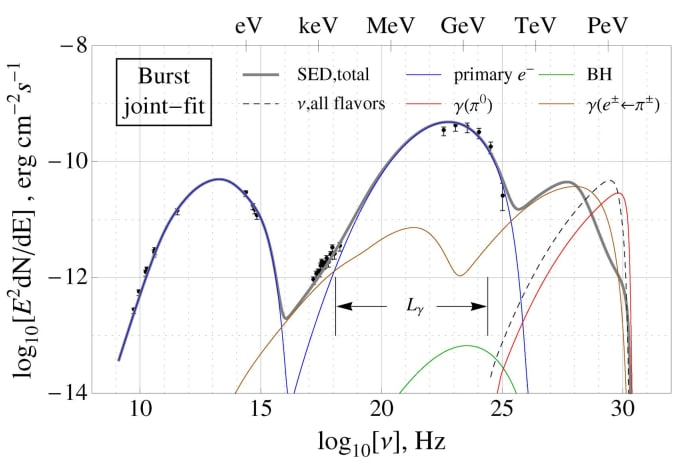
\includegraphics[width=10cm]{Plots/01_5_astroparticle/sed.jpeg}
    \caption{Different components of the blazar SED. The black dashed line on the right shows the neutrino emission spectrum around $\si{\peta\electronvolt}$ energies \cite{sed}.}
    \label{fig:sed}
\end{figure}
Accordingly, without more complex models, blazars cannot be significantly responsible for neutrinos with energies below $\si{\peta\electronvolt}$ \cite{blazar}.
Approaches for neutrinos of smaller energies include the approach of the hadronuclear channel by assuming a high particle density in the emission volume of the blazar \cite{eichmann}.
Better sources for neutrinos in the $\si{\tera\electronvolt}$ range are starburstgalaxies.

\subsection{Starburstgalaxies}
%- starburstgalaxies are galaxies with star formation at extreme levels\\
%- example: Arp 220\\
%- consists of two nuclei\\
%- star formation rate of > 100 sun mass per year\\
%- "Arp 220 is a hadronic cosmic ray calorimeter where all the power in %cosmic rays is absorbed within the nuclear starburst zones"\\
%- up to a hundred percent proton calorimeters\\
%- pp interaction -> pions -> 1.neutrino + charged lepton\\
%- flux of 1. neutrino is about $\num{6e-%12}\si{\giga\electronvolt\centi\meter\tothe{-2}\second\tothe{-1}}$ at %$\SI{0.1}{\peta\electronvolt}$\\
%\cite{starburst}
%- neutrinos from pp have a typical energy of about %$\SI{2}{\peta\electronvolt}$
%\cite{starburst2}

Apart from blazars, starburstgalaxies are candidates for the production of neutrinos of energies up to about $\SI{2}{\peta\electronvolt}$ \cite{starburst2}.
These are galaxies in which stars form at extreme levels.
One example is Arp 220, an object consisting of two nuclei surrounded by dense molecular gas.
The gas turns the object almost completely into a cosmic ray calorimeter.
Under certain model assumptions, the $pp$-interactions provide a neutrino flux for the first part of the interaction of about $\num{6e-12}\si{\giga\electronvolt\centi\meter\tothe{-2}\second\tothe{-1}}$ at $\SI{0.1}{\peta\electronvolt}$ \cite{starburst}.
The neutrino emission spectrum can be seen in figure \ref{fig:starburst} showing an emission of neutrinos in a wide energy range.
\begin{figure}
    \centering
    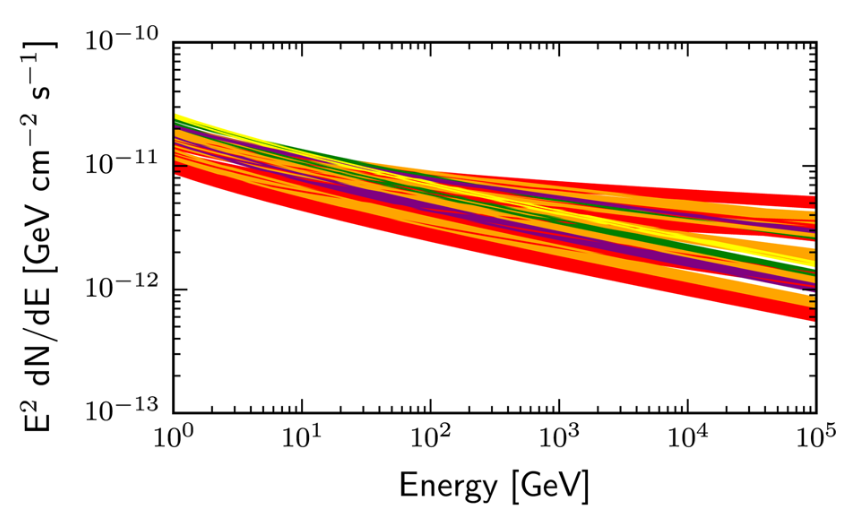
\includegraphics[width=10cm]{Plots/01_5_astroparticle/starburst_flux.png}
    \caption{Neutrino emission spectrum bands as a function of energy in starburstgalaxies. The different colours represent different combinations of fractions of the two nuclei of Arp 220 and are not important here. Important is the steady emission of low-energy to high-energy neutrinos \cite{starburst}.}
    \label{fig:starburst}
\end{figure}

\chapter{IceCube Neutrino Observatory} \label{sec:icecube}

Because of the small cross section of neutrinos, a huge detection volume is needed to detect these particles in a statistically sufficient quantity \cite{cross_n}.
Since the detection of neutrinos is based on the Cherenkov radiation of secondary particles, a detection medium is needed that is transparent to radiation in this range.
With regard to these two problems, the kilometer-thick ice at the south pole is a good choice.
The resulting IceCube neutrino observatory is the world's largest particle detector.
It is almost exactly located at the southernmost point of the earth and shown schematically in figure \ref{fig:icecube}.

\begin{figure}
    \centering
    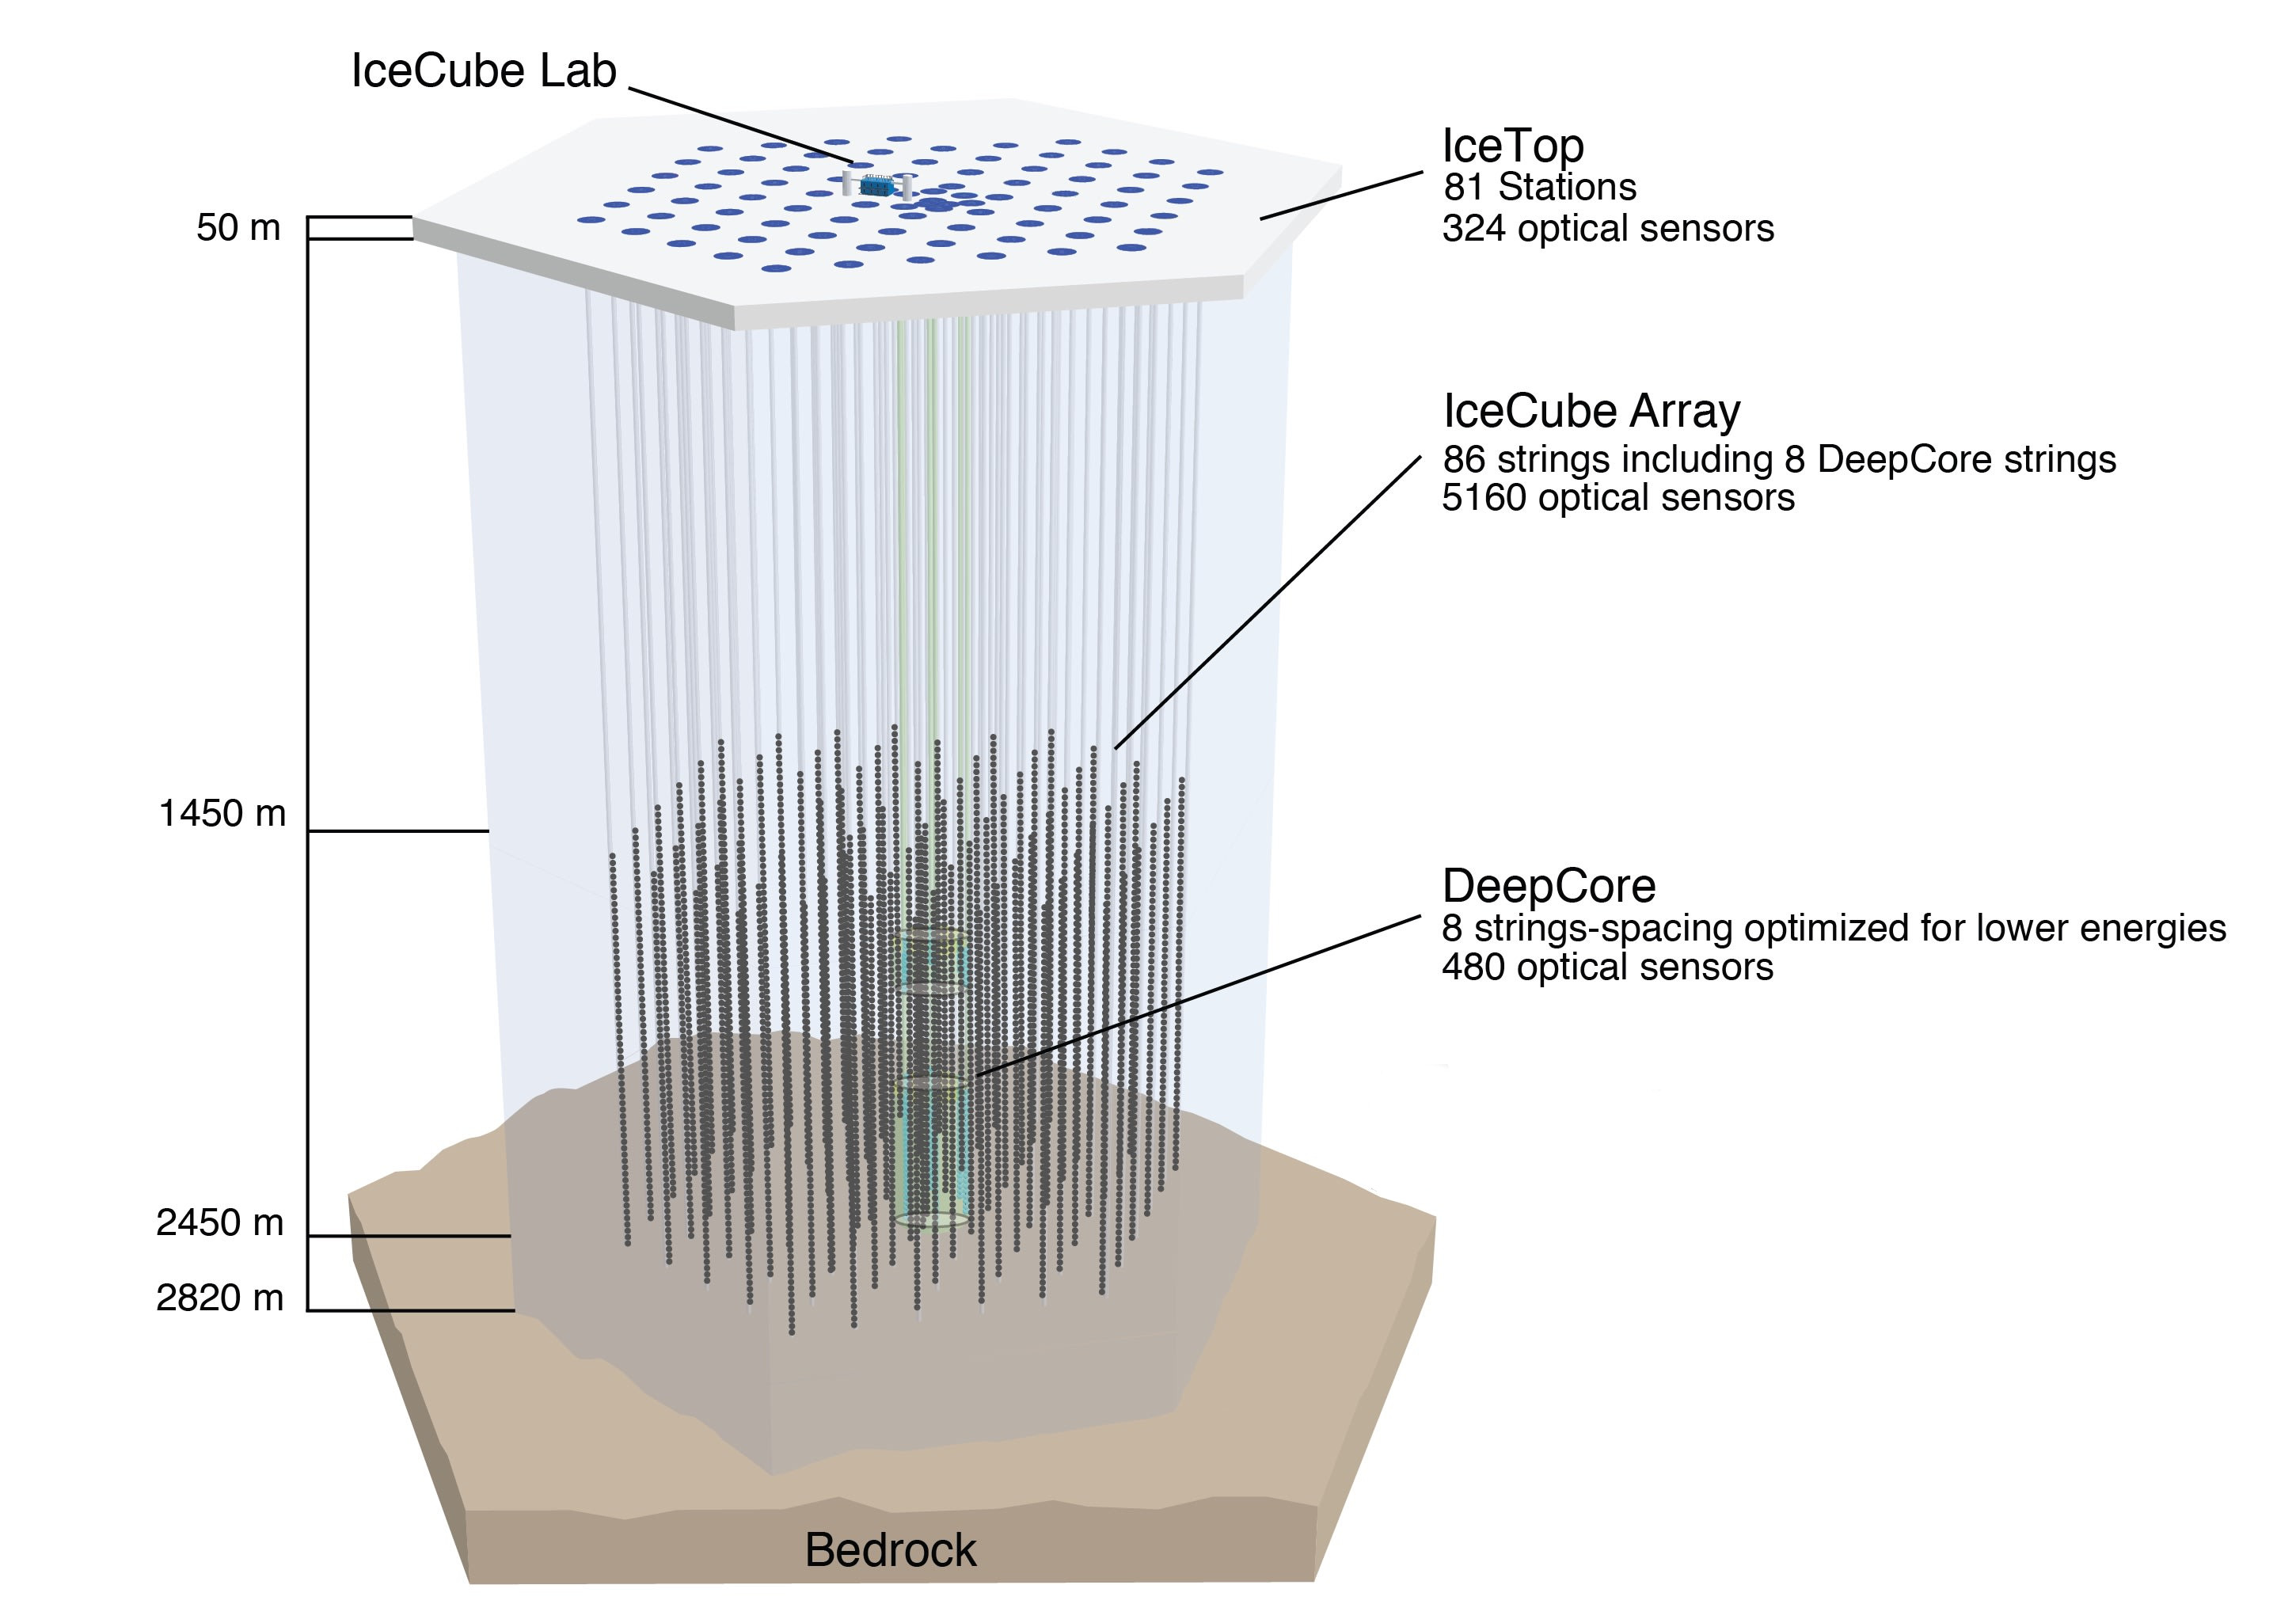
\includegraphics[width=\linewidth]{Plots/01_7_icecube/IceCube-Array.jpg}
    \caption{Schematic representation of the IceCube detector \cite{icecube_website}.}
    \label{fig:icecube}
\end{figure}

Its construction started in $\num{2004}$ and took $\num{7}$ years to its completion in $\num{2010}$.
The detector volume of IceCube covers about $\SI{1}{\kilo\meter\tothe{3}}$ of clear antarctic ice.
$\num{86}$ holes were drilled into the ice to let down cables with $\num{60}$ digital optical modules (DOMs) each.
The detection volume, or the position of the first DOM respectively, starts at a depth of about $\SI{1450}{\meter}$ and ends in a depth of about $\SI{2450}{\meter}$.
The area known as the DeepCore in the middle of the detector features a denser collection of DOMs.
IceCube detects about $\num{275}$ million cosmic rays and $\num{275}$ atmospheric neutrinos every day \cite{icecube_website}.

\section{Detection Principle}

When neutrinos interact with a medium, charged secondary particles are produced.
this occurs through a neutral current (NC) via a $Z^0$ boson or through a charged current (CC) via a $W$ boson
\begin{equation}
  \nu_l + N \xrightarrow{Z^0} \nu^{\prime}_l + X \text{ and }  \nu_l + N \xrightarrow{W} l + X, \label{eq:nc_cc_int}
\end{equation}
with $N$ and $X$ being nuclei before and after the interaction \cite{Ahlers_2018}.
If the charged secondary particles (the charged leptons $l$ in \eqref{eq:nc_cc_int}) now move through a medium at a speed faster than the speed of light in the medium, the charged secondary particles polarise the atoms along the direction of flight for a short time.
The resulting light is called Cherenkov light and is emitted at an angle of
\begin{equation}
  \Theta = \arccos{\left(\frac{1}{\beta n}\right)}, \label{eq:cherenkov}
\end{equation}
with the relativistic velocity $\beta=v/c$ of the particle and the refractive index of the medium $n$ \cite{PhysRev52378,spiering}.
A schematic representation of the Cherenkov effect is given in Figure \ref{fig:cherenkov}.
This leads to the emergence of two event signatures in the detector volume, tracks and cascades.
Tracks are produced by charged current interactions and gain their signature by the energy loss of the primary charged lepton and the secondary particles via ionization, bremsstrahlung, pair production and photo-nuclear interactions in the ice.
Cascades are created by both charged current and neutral current interactions and get their traditional signature from the rapid decay and extreme scattering of secondary particles.
\begin{figure}
  \centering
  \scalebox{0.5}{
  \begin{tikzpicture}[scale=1,
    >=stealth',
    pos=.8,
    photon/.style={decorate,decoration={snake,post length=1mm}},
    declare function={
    x1 = (sqrt(25-5*sin(45)));
    x2 = 10;
    y1 = 5*sin(45);
    y2 = 0;
    m = (5*sqrt(2)/(-20+sqrt(100-10*sqrt(2))));
    b =  (-50*sqrt(2)/(-20+sqrt(100-10*sqrt(2))));
    o = 0.5 * sqrt(25-5*sin(45));
    p = 0.5*5*sin(45);
    }
    ]
    %\draw[thick] (-3,0) -- (0,0);
    %triangle
    \draw[thick] (0,0) -- (10,0) -- (sqrt{25-5*sin{45}},5*sin{45}) -- cycle;
    \draw[thick] (0,0) -- (10,0) -- (sqrt{25-5*sin{45}},-5*sin{45});
    \draw[thick] ([shift=(0:1cm)]0,0) arc (0:67:1cm);
    \draw[thick] ([shift=(-113:1cm)]sqrt{25-5*sin{45}},5*sin{45}) arc (-113:-23:1cm);
    \node at (0.5,0.4) {$\Theta$};
    \node[mark size=1pt] at (sqrt{25-5*sin{45}} + 0.25,5*sin{45} - 0.53) {\pgfuseplotmark{*}};
    \node[scale=2] at (0.2,0.5*5*sin{45}) {$\frac{c}{n}$};
    \node[below,scale=2] at (4.5,-0.2) {$v$};
    %circles
    \draw[teal, thick] (0,0) circle (3.82);
    \draw[teal, thick] (4,0) circle (2.28);
    \draw[teal, thick] (6.5,0) circle (1.32);
    \draw[teal, thick] (8,0) circle (0.75);
    %particles
    \draw[teal,thick, ->] (10,0) -- (11,0);
    \node[mark size=2pt,teal] at (10,0) {\pgfuseplotmark{*}};
    \node[teal,scale=2] at (10,1) {$l$};
    \draw[thick,blue,photon, ->] (sqrt{25-5*sin{45}},5*sin{45}) -- node[below right,scale=2] {$\gamma$} (sqrt{25-5*sin{45}}+0.6,5*sin{45}+1.3);
    \draw[thick,blue,photon, ->] (4.9,2.1) -- (4.9+0.6,2.1+1.3);
    \draw[thick,blue,photon, ->] (7,1.25) -- (7+0.6,1.25+1.3);
    \draw[thick,blue,photon, ->] (8.3,0.7) -- (8.3+0.6,0.7+1.3);
    \draw[thick,blue,photon, ->] (sqrt{25-5*sin{45}},-5*sin{45}) -- (sqrt{25-5*sin{45}}+0.6,-5*sin{45}-1.3);
    \draw[thick,blue,photon, ->] (4.9,-2.1) -- (4.9+0.6,-2.1-1.3);
    \draw[thick,blue,photon, ->] (7,-1.25) -- (7+0.6,-1.25-1.3);
    \draw[thick,blue,photon, ->] (8.3,-0.7) -- (8.3+0.6,-0.7-1.3);
    %\draw[thick,blue,->] (sqrt{25-5*sin{45}},5*sin{45}) -- (sqrt{25-5*sin{45}}+0.5*sqrt{25-5*sin{45}},5*sin{45}+0.5*5*sin{45});
    %\draw[thick,blue,->] (sqrt{25-5*sin{45}},m*x1+b) -- (sqrt{25-5*sin{45}}+0.5*sqrt{25-5*sin{45}},m*x1+b+0.5*5*sin{45});%(5,y*(5-sqrt{25-5*sin{45}})) -- (0,0);%(5+0.2*sqrt{25-5*sin{45}},y*(5-sqrt{25-5*sin{45}}+0.2*5*sin{45}));
  \end{tikzpicture}}
  \caption{Schematic visualisation of the Cherenkov radiation $\gamma$ emitted by a charged lepton $l$ traveling with velocity $v>c/n$ through a medium with a refractive index $n$ polarizing the medium on its way. The resulting cone of Cherenkov radiation is visually comparable to the supersonic cone of an aeroplane.}
  \label{fig:cherenkov}
\end{figure}

\section{Tracks and Cascades}

To perform a point source search, two properties of the detector signatures of the muons are of particular importance: the direction and the energy.
It is therefore important to distinguish between two types of events, tracks and cascades.
Tracks pass through the detector but do not deposit all their energy in the detector volume.
This means that the direction of the event can be reconstructed very well.
The signature left by such an event can be seen in figure \ref{fig:track}.
However, since the total energy is not deposited in the detector volume, the reconstruction of the energy is generally not optimal.
\begin{figure}
    \centering
    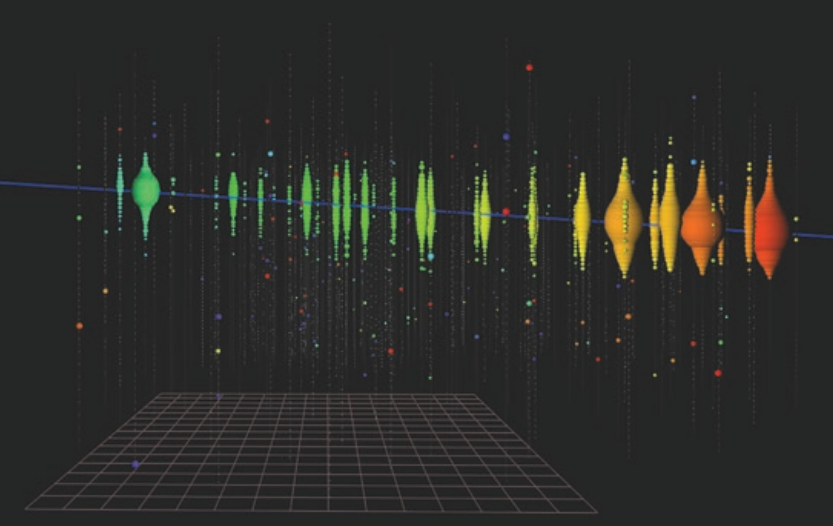
\includegraphics[width=10cm]{Plots/01_7_icecube/track.png}
    \caption{Tracklike event signature in the detectorvolume. The deposited energy is represented by the size of the spheres, the time of arrival by the colour (red earlier, blue later). The small glow of individual modules is unfiltered noise \cite{spiering}.}
    \label{fig:track}
\end{figure}

Cascades, on the other hand, deposit their entire energy in the detector volume, which means that the energy can be determined quite accurately.
Due to the shape of the cascade event, however, the original direction is very difficult to reconstruct.
Such an event can be seen in figure \ref{fig:cascade}.
Generally, the magnitude of the event's energy is the main statistical indicator of whether an event is astrophysical in origin, but the exact reconstruction of the event's direction is very important for a point source search.
Therefore, a dataset from tracks is usually used.
However, due to their high energy, cascade events can be used as a source catalogue \cite{steve_und_mirco}, but this is not the case in this thesis.
\begin{figure}
    \centering
    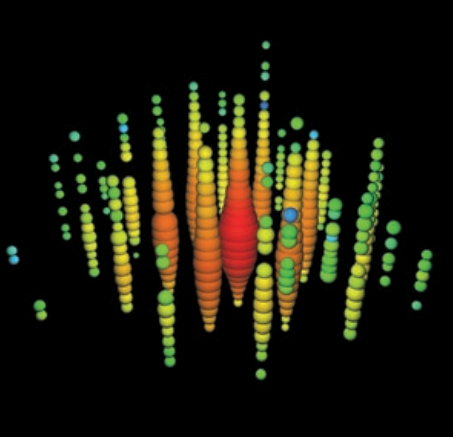
\includegraphics[width=10cm]{Plots/01_7_icecube/cascade.png}
    \caption{The filtered cascade event nicknamed \textit{Ernie} with a reconstructed energy of $\SI{1.04}{\peta\electronvolt}$. The deposited energy is represented by the size of the spheres, the time of arrival by the colour (red earlier, blue later) \cite{spiering}.}
    \label{fig:cascade}
\end{figure}

%theory
\chapter{Point Source Searches in IceCube} \label{sec:theory}

This chapter provides an insight into the theoretical formulas, principles and software used to perform a point source analysis.
The theoretical background gives a basic impression of the calculation and is necessary for understanding chapter \ref{sec:tdepps}, where the general calculation of the test statistic is discussed.

\section{Modelling the Test Statistic}

A point source search consists of a hypothesis test based on two hypotheses \cite{likelihood_method}.
The null hypothesis $H_0$ states that the examined data consist only of atmospheric background, while the hypothesis $H_\text{S}$ states that the data consist of background and astrophysical neutrino events, the latter emitted by a source of certain properties.
The hypothesis $H_\text{S}$ uses the parameter space $\Theta$ while the null hypothesis only uses a subset of this parameter space $\Theta_0$.
The hypothesis test is the quotient of the underlying likelihoods $\CL$ of the hypotheses,
\begin{equation}
  \Lambda = \frac{\CL_{\Theta_0}}{\CL_\Theta}.
\end{equation}
Since the hypothesis $H_\text{S}$ contains the null hypothesis, the test statistic $TS$ can be expressed via Wilks' theorem \cite{wilk} as
\begin{equation}
  TS = -2\ln\hat{\Lambda} = 2\ln\Gb{\sup_{\theta\in\Theta}\CL(\theta)} - 2\ln\Gb{\sup_{\theta\in\Theta_0}\CL(\theta)}, \label{eq:TS}
\end{equation}
with the set $\theta$ of parameters that maximizes the likelihoods.
The test statistic now follows a $\chi^2$ distribution, given that the sample size is large enough.
In point source searches, the likelihoods are defined as
\begin{equation}
  \CL(\lambda) = \frac{\lambda^Ne^{-\lambda}}{N!}\prod^N_{i=1}P_i
\end{equation}
or
\begin{equation}
  \ln\CL(\lambda) = -\lambda + \sum^N_{i=1}\ln{(\lambda P_i)}
\end{equation}
in the the logarithmic form \cite{ex_likelihood} dropping the $\ln(N!)$ term, where $\lambda$ is the number of expected events and $N$ is the total number of individual events $i$.
$P_i$ defines the per-event model distributions giving the probabilities for each event.
In the case of stacking several sources $k$, the number of expected events is divided and the formula
\begin{equation}
  \ln\CL(\{\lambda_k\}) = -\sum^{N_\text{srcs}}_{k=1}\lambda_k + \sum^{N_\text{evts}}_{i=1}\ln{\Gb{\sum^{N_\text{srcs}}_{k=1}\lambda_k P_{i,k}}},
\end{equation}
is obtained.
If the likelihoods are inserted into formula \eqref{eq:TS}, the general formula for the test statistic is derived,
\begin{equation}
    TS = -2\ln{\hat\Lambda} = -2\sum_{k=1}^{N_{\text{srcs}}}\hat\lambda_{k,S} + 2\sum_{i=1}^{N_{\text{evts}}}\ln{\Gb{\frac{\sum_{k=1}^{N_{\text{srcs}}}\hat\lambda_{k,S}S_{i,k}}{\sum_{k=1}^{N_{\text{srcs}}}\langle\lambda_{k,B}\rangle B_{i,k}}+1}}, \label{eq:TS_general}
\end{equation}
where $\hat\lambda$ maximizes the test statistic value.
The expected number of background events $\langle\lambda_{k,B}\rangle$ is estimated a priori integrated over the rate of background events.

The further form of the test statistic depends on the choice of probability models $S$ and $B$.
If a time-integrated search or a search in which the sources are independent of each other in terms of different temporal intervals is carried out, the formula simplifies to
\begin{equation}
    TS = -2\sum_{k=1}^{N_{\text{srcs}}}\hat\lambda_{k,S} + 2\sum_{i=1}^{N_{\text{evts}}}\sum_{k=1}^{N_{\text{srcs}}}\ln{\Gb{\frac{\hat\lambda_{k,S}S_{i,k}}{\langle\lambda_{k,B}\rangle B_{i,k}}+1}}. \label{eq:ts_simple}
\end{equation}
This makes it possible to form per-event probability density functions (PDF) ratios directly in the calculation, which reduces the computational effort.

There is some software available to practically perform a point source search.
Among the best known are \texttt{SkyLLH}\footnote{\url{https://github.com/icecube/skyllh}}, \texttt{skylab}\footnote{\url{https://github.com/icecube/skylab}} and \texttt{csky}\footnote{\url{https://github.com/icecube/csky}, private repository}.
The software \texttt{csky}, which is used in this thesis, is easy to use and, due to the outsourcing of computationally intensive steps to \texttt{C++}, a time-efficient calculation in comparison to the other mentioned softwares, which are implemented entirely in \texttt{Python}.

\section{Likelihood in csky}

The likelihood of a source in \texttt{csky} is shown in the equation below,
\begin{equation}
  \CL(n_s,\Vmu)
  = \prod_i \Gb{
    \frac{n_s}{N} \CS(\Vx_i|\Vmu)
    + \Gp{1 - \frac{n_s}{N}} \CB(\Vx_i)
  },
  \label{eq:lh}
\end{equation}
with the total number of events $N$, the event parameters $\Vx_i$ and the analysis parameters
\begin{align}
  \Vmu &= \{\text{number of signal events }n_S, \text{ spectral index }\gamma\},
\end{align}
where $\Vmu$ will be optimised\footnote{A representation of the likelihood can be found directly in the \texttt{csky} software package.}.
The probability functions of the individual events are broken down into three different parts according to the event parameters, an energy, a spatial and a temporal PDF.
However, the temporal PDF is only important for time-dependent searches,
\begin{align}
  \CS(\Vx|\Vmu)
  &= \CS_S(\delta,\alpha)
  \cdot \CS_E(E|\Vmu)
  \cdot \CS_T(t|\Vmu), \label{eq:signal_pdfs}
  \\
  \CB(\Vx)
  &= \CB_S(\delta)
  \cdot \CB_E(E)
  \cdot \CB_T(t).
  \label{eq:background_pdfs}
\end{align}
The energy PDF can be constructed of a 2d histogram of energy and declination and is generated directly from the data for the background $\CB_E(E)$ and from simulations weighted with the spectral index $\gamma$ for the signal $\CS_E(E|\Vmu)$.
Its ratio does not depend on individual event properties and is a priori calculated.
The spatial PDF of the signal $\CS_S(\delta,\alpha)$ depends on the declination and right ascension of the event and corresponds to a Kent distribution around the position of the source.
The Kent distribution is the equivalent of a normal distribution on a sphere \cite{kent}.
The background PDF $\CB_S(\delta)$, on the other hand, is obtained directly from the spatial distribution of the data, since most events are background events.
It depends only on the declination since the background is generally uniformly distributed in the sky and the distribution depends merely on the absorption of the earth.
The temporal PDF in the case of this thesis is a simple box function, equal for both signal and background, that corresponds to $\CS_T(t|\Vmu)=1$ over a certain time interval.
Only events that fall within this time window contribute.

\section{Calculating Sensitivity and Discovery Potential}

Sensitivity and discovery potential are defined by the number of signal events that must be injected so that the resulting test statistic is $\SI{90}{\percent}$ above the median of the background statistic or $\SI{50}{\percent}$ above $\num{5}\sigma$ of the latter respectively.
These conditions can be seen schematically in figure \ref{fig:sens_disc_schem}.
\begin{figure}\centering
  \begin{tikzpicture}[
declare function={gamma(\z)=
2.506628274631*sqrt(1/\z)+ 0.20888568*(1/\z)^(1.5)+ 0.00870357*(1/\z)^(2.5)- (174.2106599*(1/\z)^(3.5))/25920- (715.6423511*(1/\z)^(4.5))/1244160)*exp((-ln(1/\z)-1)*\z;},
declare function={gammapdf(\x,\k,\theta) = 1/(\theta^\k)*1/(gamma(\k))*\x^(\k-1)*exp(-\x/\theta);}]
\begin{axis}[ymode=log, ymin=0,
no markers, domain=0:9, samples=100,
axis lines=left, xlabel=$\text{TS}$, ylabel=$\#\text{trials}$,
y label style={at={(axis description cs:0.1,.5)},anchor=north},
x label style={dashed,at={(axis description cs:0.95,0.05)},anchor=west},
height=5cm, width=9cm,
xtick={6,14.87}, ytick=\empty,
xticklabels={$\text{bg median}$,$5\sigma$},
%xticklabels={$\bar n (\theta_t)$},
enlargelimits=false, clip=false,% axis on top,
grid = major]
\addplot [very thick,cyan!20!black,domain=0:20, draw=none] {gammapdf(x,0.2,5)};
\addplot [very thick,cyan!20!black,domain=0.5:19.5] {gammapdf(x,0.2,5)};
%\addplot [domain= 0.5:4.5]{gauss(2.5,0.6,2)};
%\addplot [fill=cyan!20, draw=none, domain=0:6.0] {gammapdf(x,2,2)} \closedcycle;
%\addplot [very thick, fill=white!20!white, draw=none, domain=6.01:20] {gammapdf(x,2,2)} \closedcycle;
\end{axis}
\node at (2.5,1.7) {\begin{tikzpicture} \begin{axis}[hide axis,enlargelimits=false, ymax = 1,height=5cm, width=4cm,domain=2.65:3.35]\addplot [domain= 2.65:3.35,smooth,thick,green]{gauss(3,0.1,0.2)}; \end{axis} \end{tikzpicture}};
\node at (5.5,1.7) {\begin{tikzpicture} \begin{axis}[hide axis,enlargelimits=false, ymax = 1,height=5cm, width=3.5cm,domain=2.7:3.3]\addplot [domain= 2.7:3.3,smooth,thick,red]{gauss(3,0.07,0.14)}; \end{axis} \end{tikzpicture}};
\node[green] at (2.7,3) {$\xrightarrow{\text{90\%}}$};
\node[red] at (6,3) {$\xrightarrow{\text{50\%}}$};
\node at (0.5,3) {$\text{bg}$};
\node[green] at (2.7,4) {$\text{sensitivity}$};
\node[red] at (6,4) {$\text{discovery}$};
\end{tikzpicture}
\caption{Schematic showing the conditions to calculate the sensitivity and discovery potential. The background test statistic is shown in black, the signal test statistic satisfying the sensitivity conditions in green and the one for the discovery potential in red. Note that the curves do not actually look like those shown here. They have been simplified for explanatory purposes.}
\label{fig:sens_disc_schem}
\end{figure}
Let the number of sufficient signal events then be $N_\text{sig}$, the sensitivity $sens$ and discovery potential $disc p$ then are
\begin{align}
  sens &= \frac{N_\text{sig,sens}}{A_\text{det}}E_0, \label{eq:sens}\\
  disc p &= \frac{N_\text{sig,disc p}}{A_\text{det}}E_0, \label{eq:disc}
\end{align}
with the total signal acceptance of the detector $A_\text{det}$ and the reference energy $E_0$.
The time-dependent sensitivity and discovery potential are given in a fluence rather than a flux.% by multiplying with $E_0^2$, these results can then be compared to other analyses.

%sources
\chapter{Source Selection}
%general: cascades and tracks\\
what are the best sources and why\\
probability of being of astrophysical origin\\
History of EHE, HESE to bronze, gold alerts Thomas Kintschers gfu\\
what is a gfu\\
hängt ab von zen, dec, track\_len, bdt\_up (upgoing oder nicht) oder bei donwgoing: truncated energy, qtot (deponierte Ladung)\\
\_zen\_cut = np.radians(82.)\\
up: pass\_gold[m]   = pass\_precut[m] \& (qtot[m] > 10.\*\*np.polyval(\_coeff2, np.sin(dec[m])))\\
\_coeff2 = [  -4.06580, -10.60906,  -9.61048,   3.01219 ]\\
down: pass\_gold[m]   \= pass\_precut[m] \& (logTruncated[m] > \_cut2)\\
\_cut2   = 5.14\\

table of sources, skymaps\\

%data
\chapter{Dataset}
which dataset to use and why\\
description of the set: table of various info (livetime, number of events)\\
mention overlap in time due to testruns\\
removing sources from data and mc\\
mention icetray modules, my ehe\_collector\_v2 maybe\\
mention ehealertfilter being totally busted\\
show sindec distribution of mc and filtered mc, maybe sindec-energy 2d hist\\
mention weighting (Powerlawflux)\\

%csky stuff
\chapter{Time-Integrated Search}

This chapter describes the time-integrated stacking search, starting with the properties of the analysis, followed by a description of the background trials and finally the signal trials with the result of the sensitivity and the discovery potential.
The search covers different spectral indices for the signal event emission.

\section{Analysis properties}

This section shows some of the underlying PDFs csky uses to calculate the test statistic values.
Since csky is based on PDF ratios for practical reasons, not all individual PDFs can be shown clearly.
Consequently, here are a few basic PDFs and ratios whose form is apriori important for the quality of the analysis.

\subsection{Background space PDF}

The background space PDF is generated with data and only depends on the declination $\delta$ of the events, given by the almost right ascension symmetry of the IceCube detector due to its position.
It is normalized over the whole sky, hence satisfying the condition
\begin{align}
  \int d\Omega f = \int d\alpha \int d(\sin(\delta)) f = 1
\end{align}
and is shown in figure \ref{fig:bg_param_time_int}.
Lastly a spline, interpolating between the bin centers, is used to evaluate the events.
\begin{figure}
    \centering
    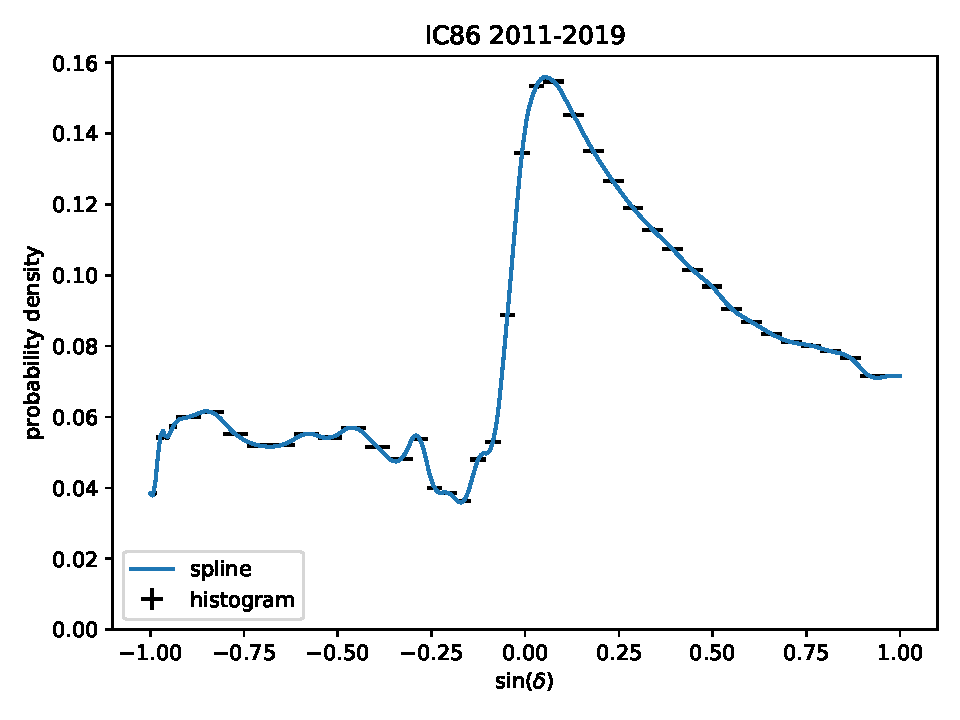
\includegraphics[width=\linewidth]{Plots/05_csky/bg_space_pdf.pdf}
    \caption{Background space PDF used in this analysis in $\sin{(\delta)}$ for all $\num{9}$ years, 2011-2019.}
    \label{fig:bg_param_time_int}
\end{figure}
The background space parametrization results in one plot only because all datasets underwent the same data processing pipeline.
The PDF shows a lower contribution for downgoing events and a higher one for upgoing events coming from the sides.
This result is compatible with other analyses, for example ...

\subsection{Energy ratio PDF}

The energy PDF ratios for different spectral indices $\gamma$ can be seen in figure \ref{fig:energy_ratio_time_int}.

\begin{figure}
    \centering
    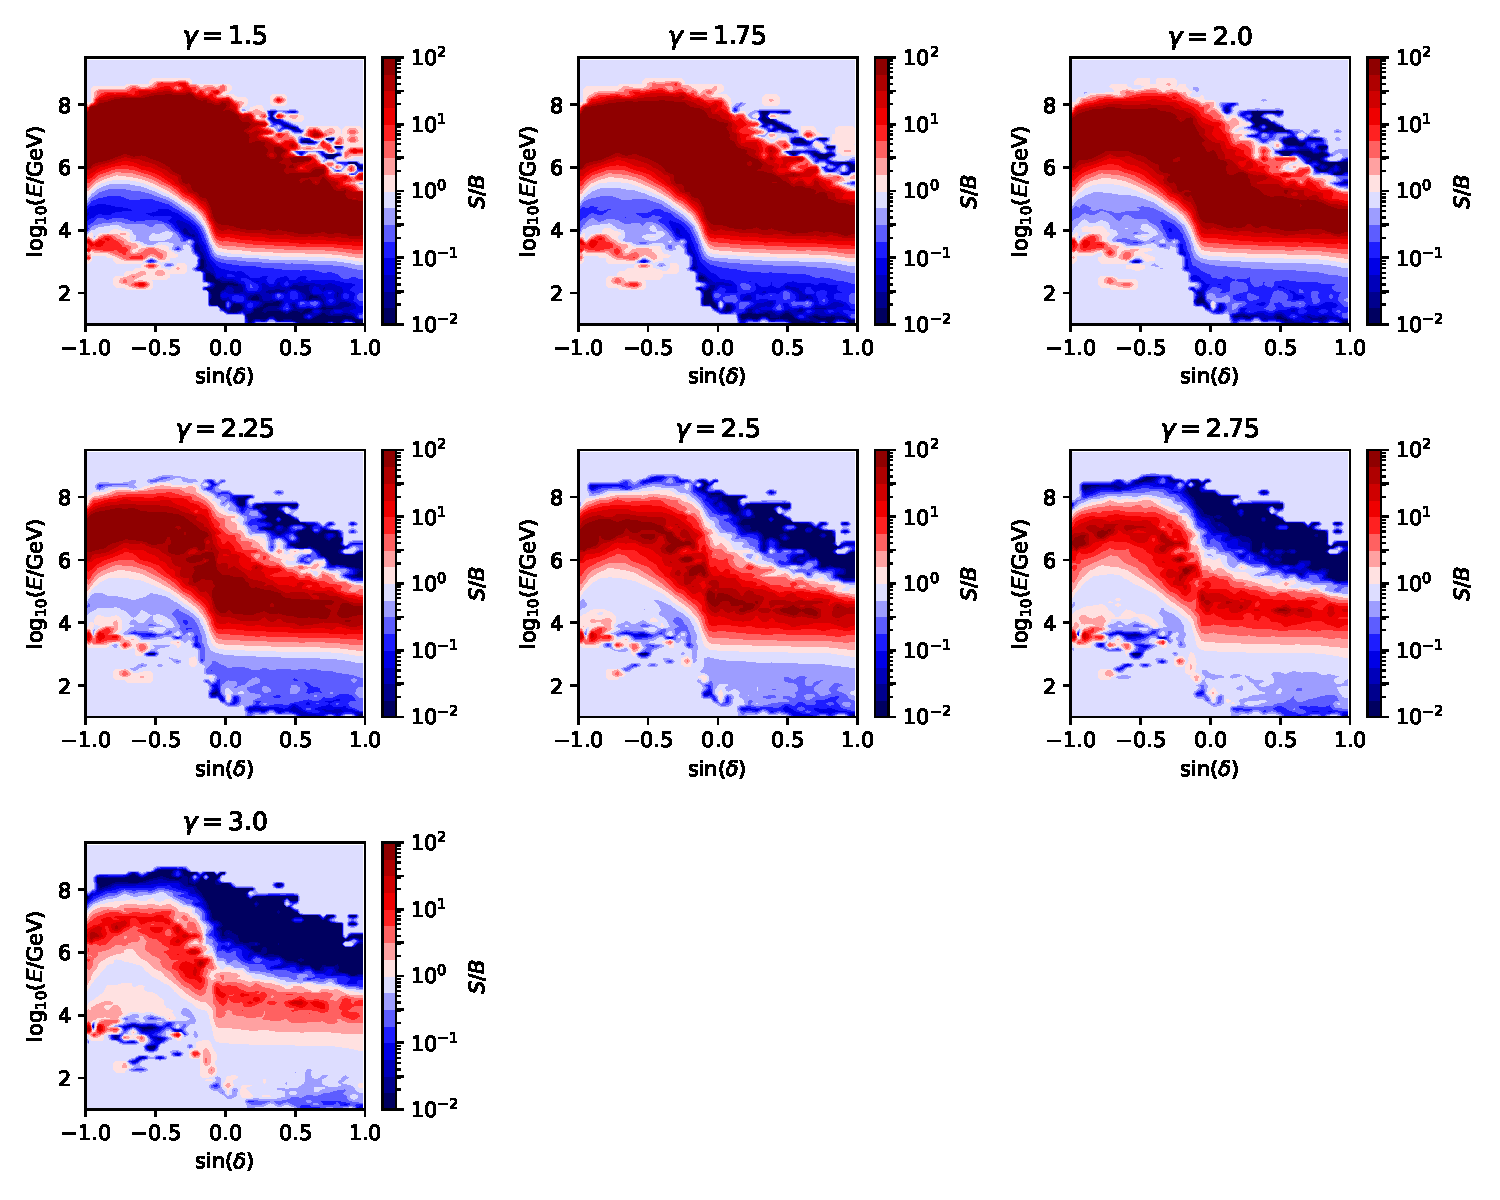
\includegraphics[width=\linewidth]{Plots/05_csky/energy_pdf_ratio.pdf}
    \caption{Energy PDF ratios used in this analysis in $\sin{(\delta)}$ and $\sin{\log{(E)}}$ for all $\num{9}$ years, 2011-2019, for different spectral indices $\gamma$.}
    \label{fig:energy_ratio_time_int}
\end{figure}

Mention high values in upper right (okay since they bias towards lower sens values (weaken)) and lower left (bad, bias towards higher sens values)

\section{Background Trials}

mention stacking

The histogram of the background test statistic values can be seen in figure \ref{fig:bg_ts_time_int}.
The number of trials processed is $\num{974000}$\footnote{Originally $\num{e6}$, but some jobs fail due to various technical reasons.}.
Important features of the plot are that the $\chi^2$ distribution has as straight a tail as possible.
This is reflected in the number of degrees of freedom $dof$ in the $\chi^2$ distribution.
This should be as close to 1 as possible, which corresponds to a pure background statistic without signal.
The test statistic should also be symmetrical around the zero point.
A shift around the zero point is an indication of an undesired bias of the statistic.
Therefore, the value of the quotient of the number of positive and negative events should ideally be $\eta = \num{0.5}$.
Apart from the fit parameters, the median and $5\sigma$ deviation value of the test statistic are necessary for the subsequent calculation of the sensitivity and the discovery potential.

The fit parameters of the background test statistic are
\begin{align}
  dof &= \num{1.115},\\
  \eta &= \num{0.656}
\end{align}
and the key values later to be processed are as follows\footnote{Some analyses use the $3\sigma$ value for the discovery potential.}
\begin{align}
  median &= \num{0.140},\\
  3\sigma &= \num{10.651},\\
  5\sigma &= \num{28.060}.
\end{align}

\begin{figure}
    \centering
    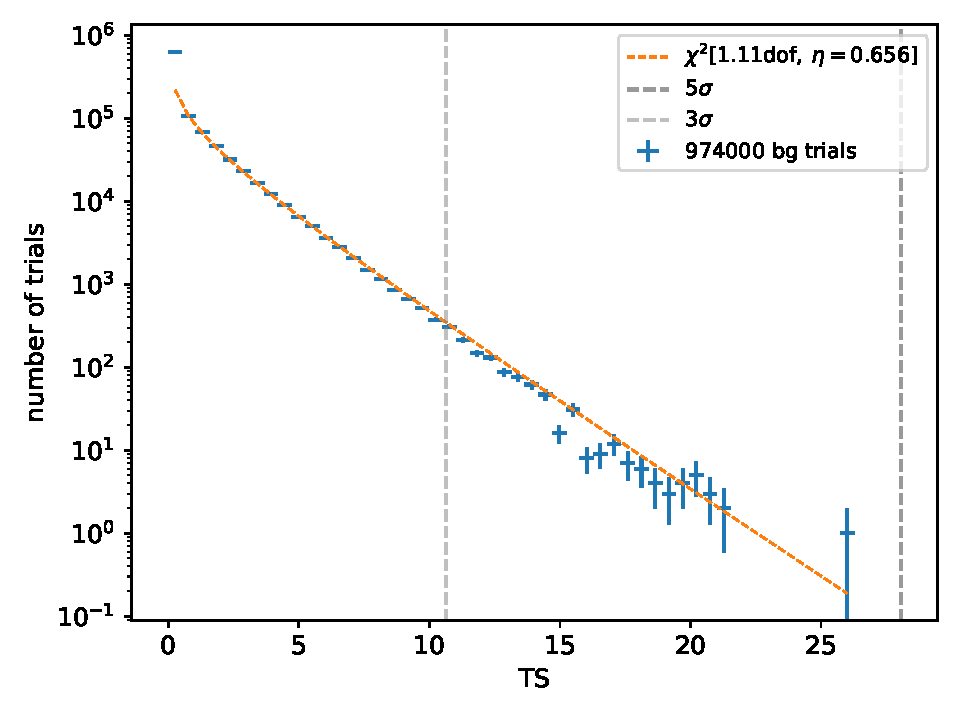
\includegraphics[width=\linewidth]{Plots/05_csky/9_years_gfu_gold_bg_new.pdf}
    \caption{Histogram of the background test statistic for the time integrated analysis. Shown are also the number of degrees of freedom $dof$ and the ratio of positive and negative values $\eta$.}
    \label{fig:bg_ts_time_int}
\end{figure}

\section{Signal Trials}

Before calculating the sensitivities and discovery potentials, certain properties of the likelihood or its behaviour should be investigated.
Since the spectral index $\gamma$ and the signal parameter $n_\text{S}$ are fitted, it is advisable to look at the likelihood environment to check for a smooth landscape to ensure a fit is possible and to exclude any other unwanted local maxima.
A scan of the parameter space for one likelihood can be seen in figure \ref{fig:llh_scan_time_int}.
Although there is a relatively flat maximum, the likelihood environment does not show any strange behaviour.
\begin{figure}
    \centering
    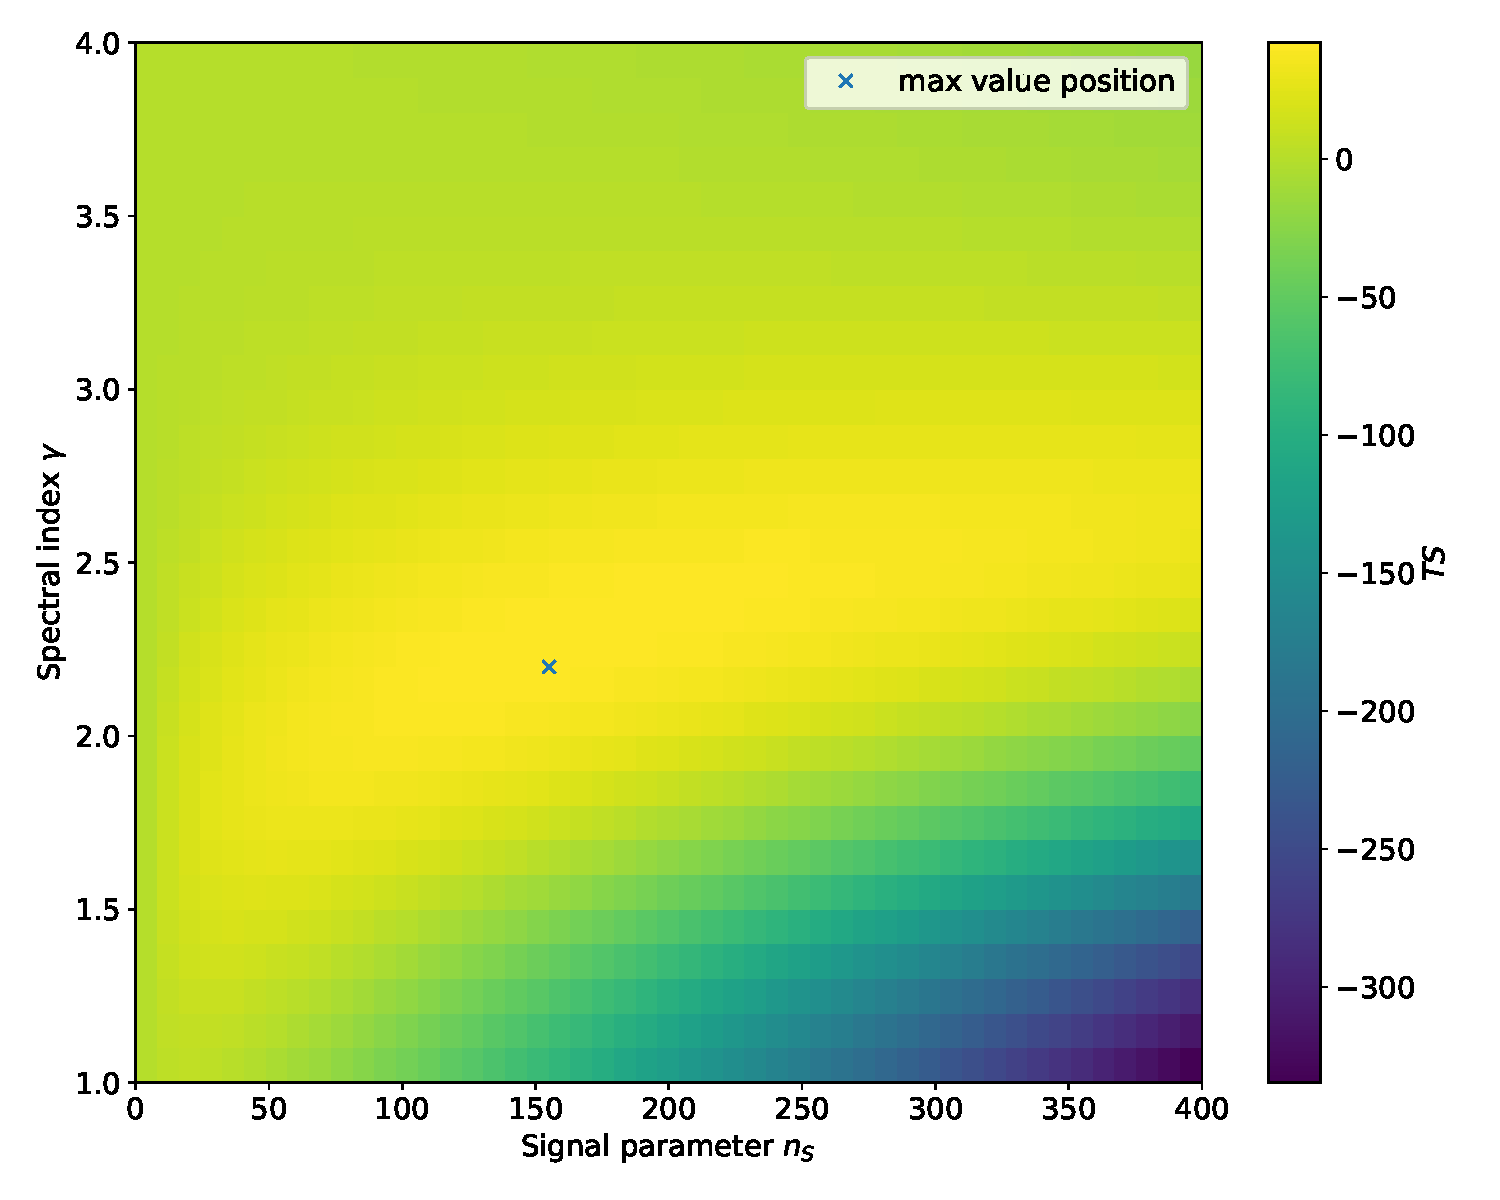
\includegraphics[width=\linewidth]{Plots/05_csky/llh_scan_time_int.pdf}
    \caption{Scan of one likelihoodspace for the time integrated analysis in the spectral index $\gamma$ and the signal parameter $n_\text{S}$. The number of induced signal events is $n_S = \num{100}$ with a spectral index of $\gamma = 2$. The maximum test statistic value is marked in the plot including the contours of $\num{1}\sigma$ and $\num{2}\sigma$.}
    \label{fig:llh_scan_time_int}
\end{figure}
The method of the calculation of the contours comes from \cite{Blobel} and corresponds to the maximum of the negative log-likelihood after subtracting $\num{0.5}$ and $\num{2}$ accordingly to get the $1\sigma$ and $2\sigma$ range, respectively.

After the fit behaviour has been checked, the signal can be injected.
With a higher number of signal events, the test statistic shifts to higher values, eventually reaching the thresholds set for the sensitivity and discovery potential.
Practically csky provides methods to apriori get an estimation of the number of signal events that have to be injected to satisfy certain thresholds without having to run a lot of trials on a cluster first.
The determined list of the number of signal events injected for the trials can be seen in table \ref{tab:signal_injected}.
The resulting CDFs for the time integrated sensitivities and discovery potentials can be seen in figure \ref{fig:cdf_sens} and \ref{fig:cdf_disc}.
Each point corresponds to the percentage of the test statistic being passed the thresholds mentioned in chapter \ref{sec:theory}.
\begin{figure}
    \centering
    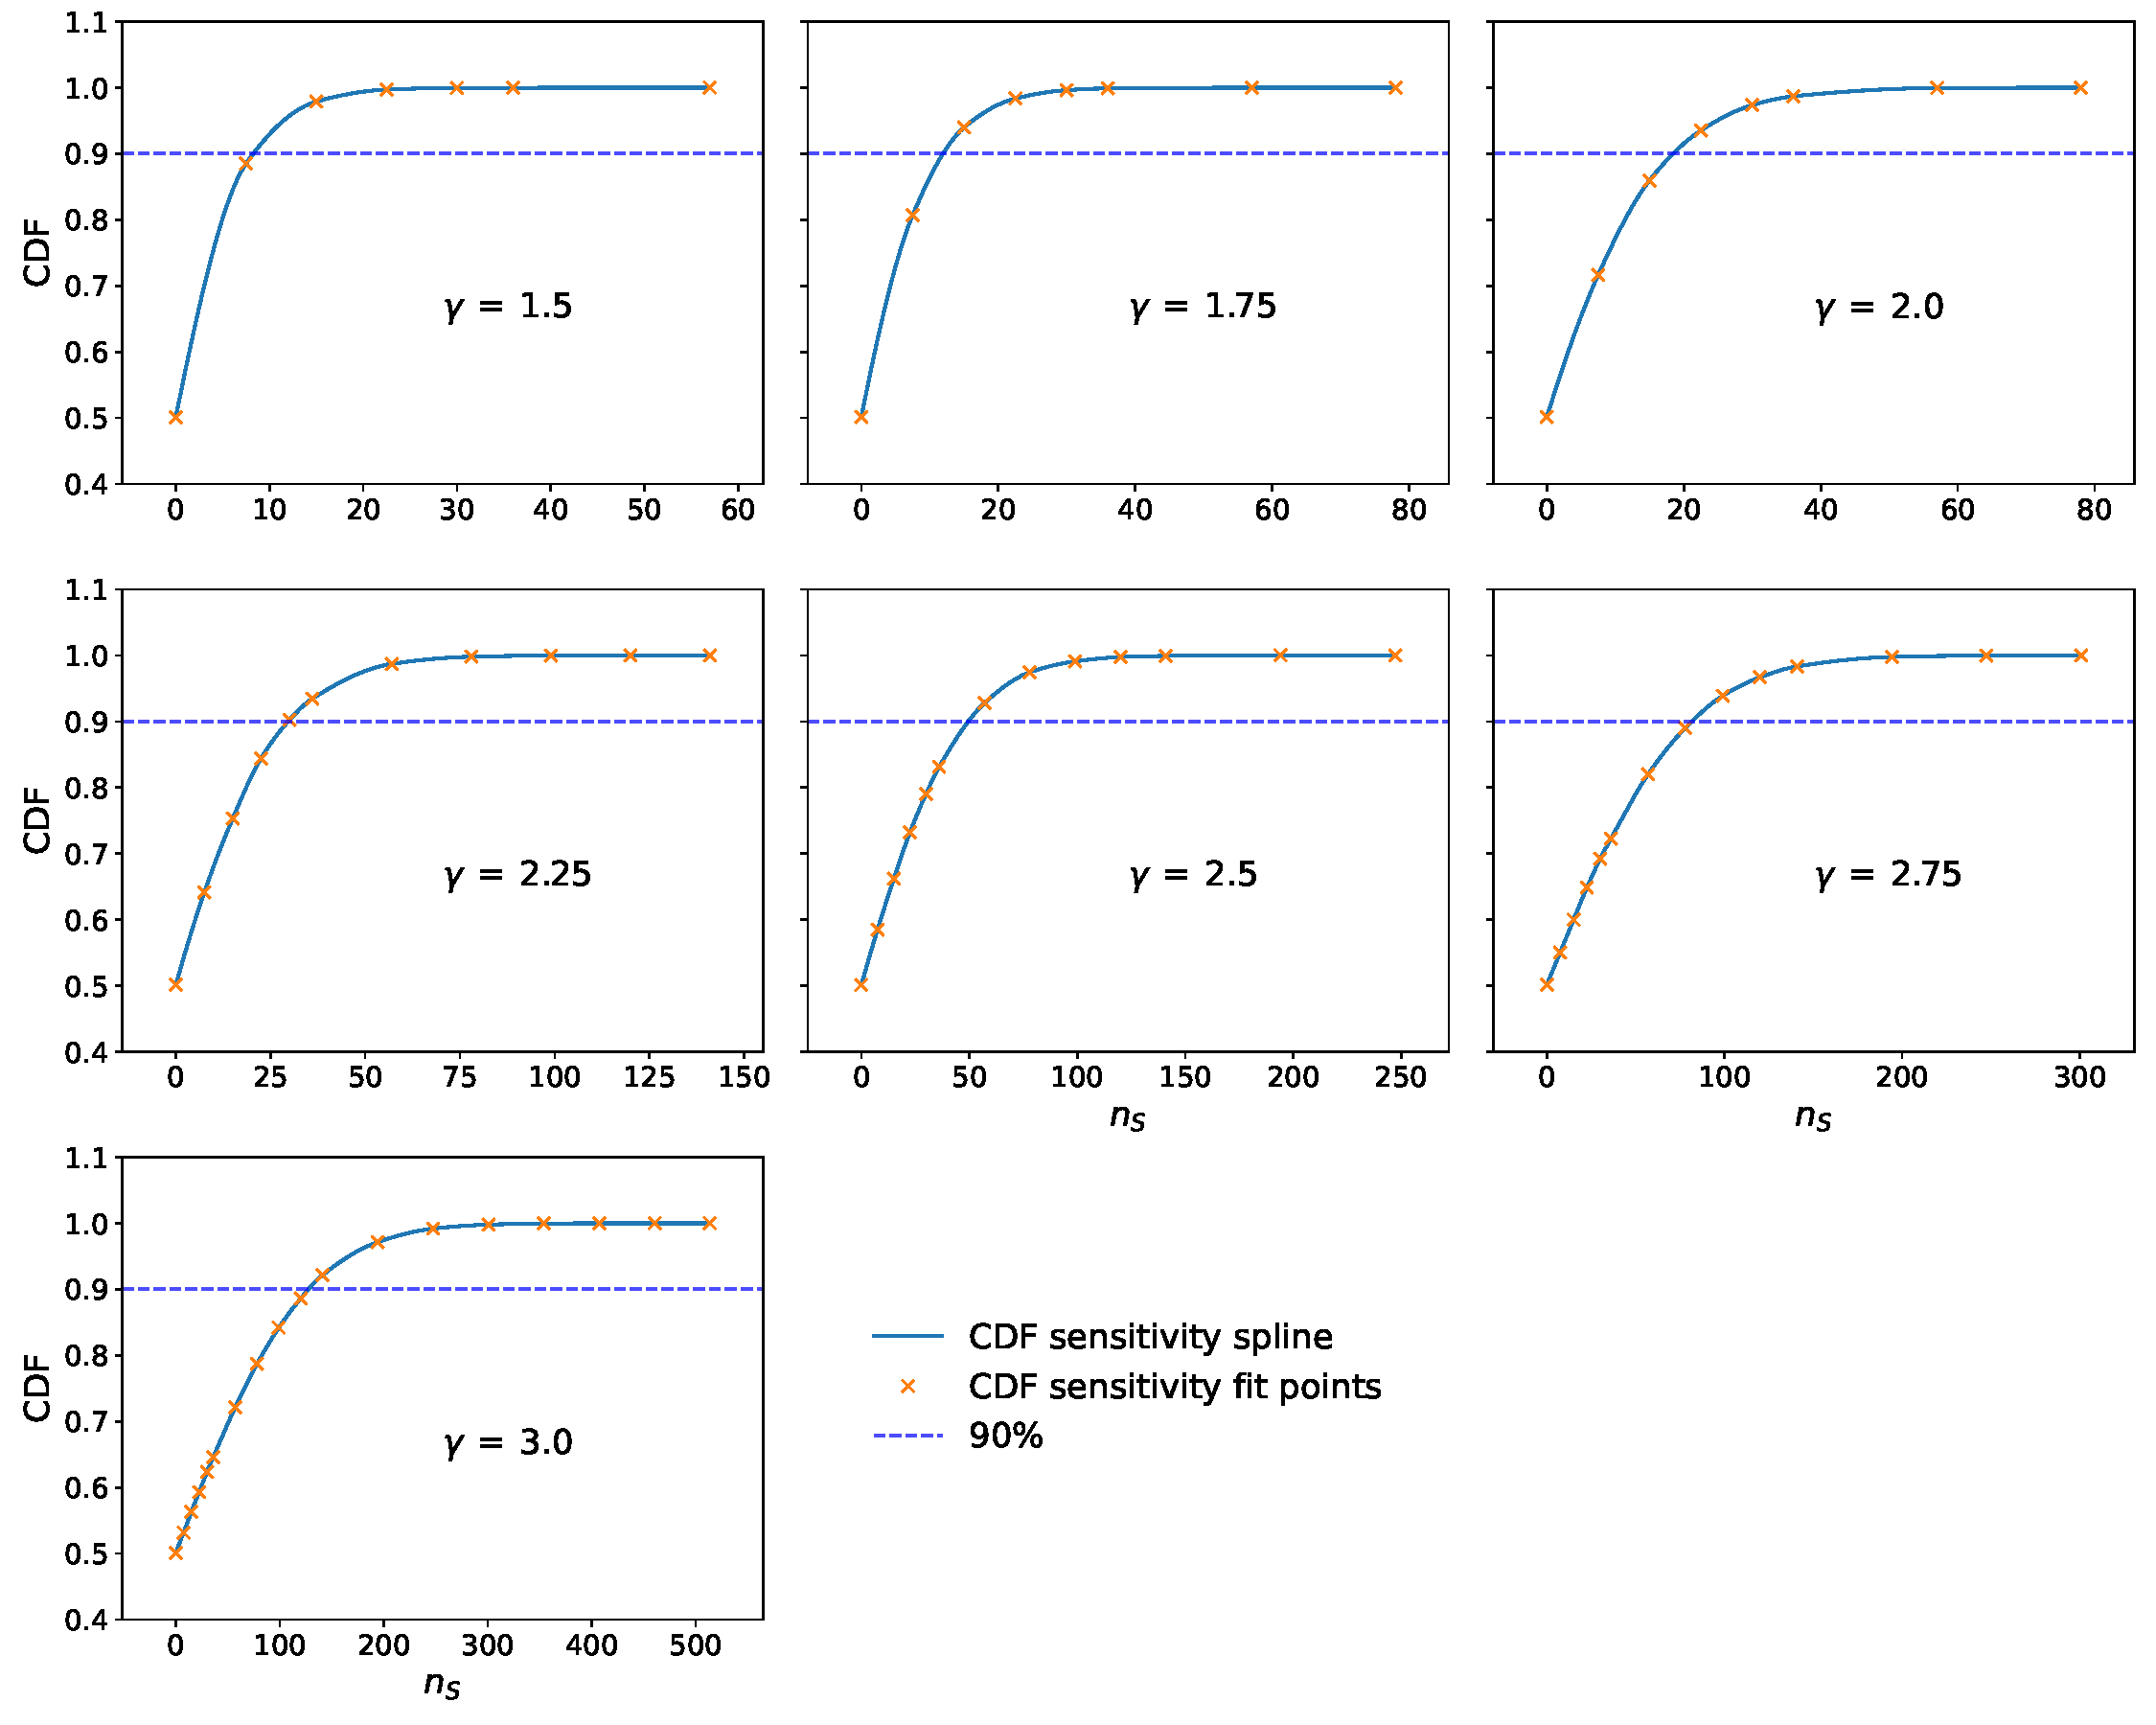
\includegraphics[width=\linewidth]{Plots/05_csky/9_years_gfu_gold_cdf_sens.pdf}
    \caption{Quantiles of the signal trials for the calculation of the sensitivity for the time integrated analysis at different spectral indices $\gamma$. A $\chi^2$ CDF fit provides a more accurate estimate of the sought signal parameter $n_\text{S}$ which satisfies the sensitivity condition at $\SI{90}{\percent}$.}
    \label{fig:cdf_sens}
\end{figure}
Note that all plots in figure \ref{fig:cdf_sens} start at about $\SI{50}{\percent}$ with a signal parameter of $n_\text{S} = 0$.
Since the absence of a signal parameter produces the background test statistic, the statistics share the same median, hence there will always be $\SI{50}{\percent}$ of the signal test statistic above the median of the background test statistic.
\begin{figure}
    \centering
    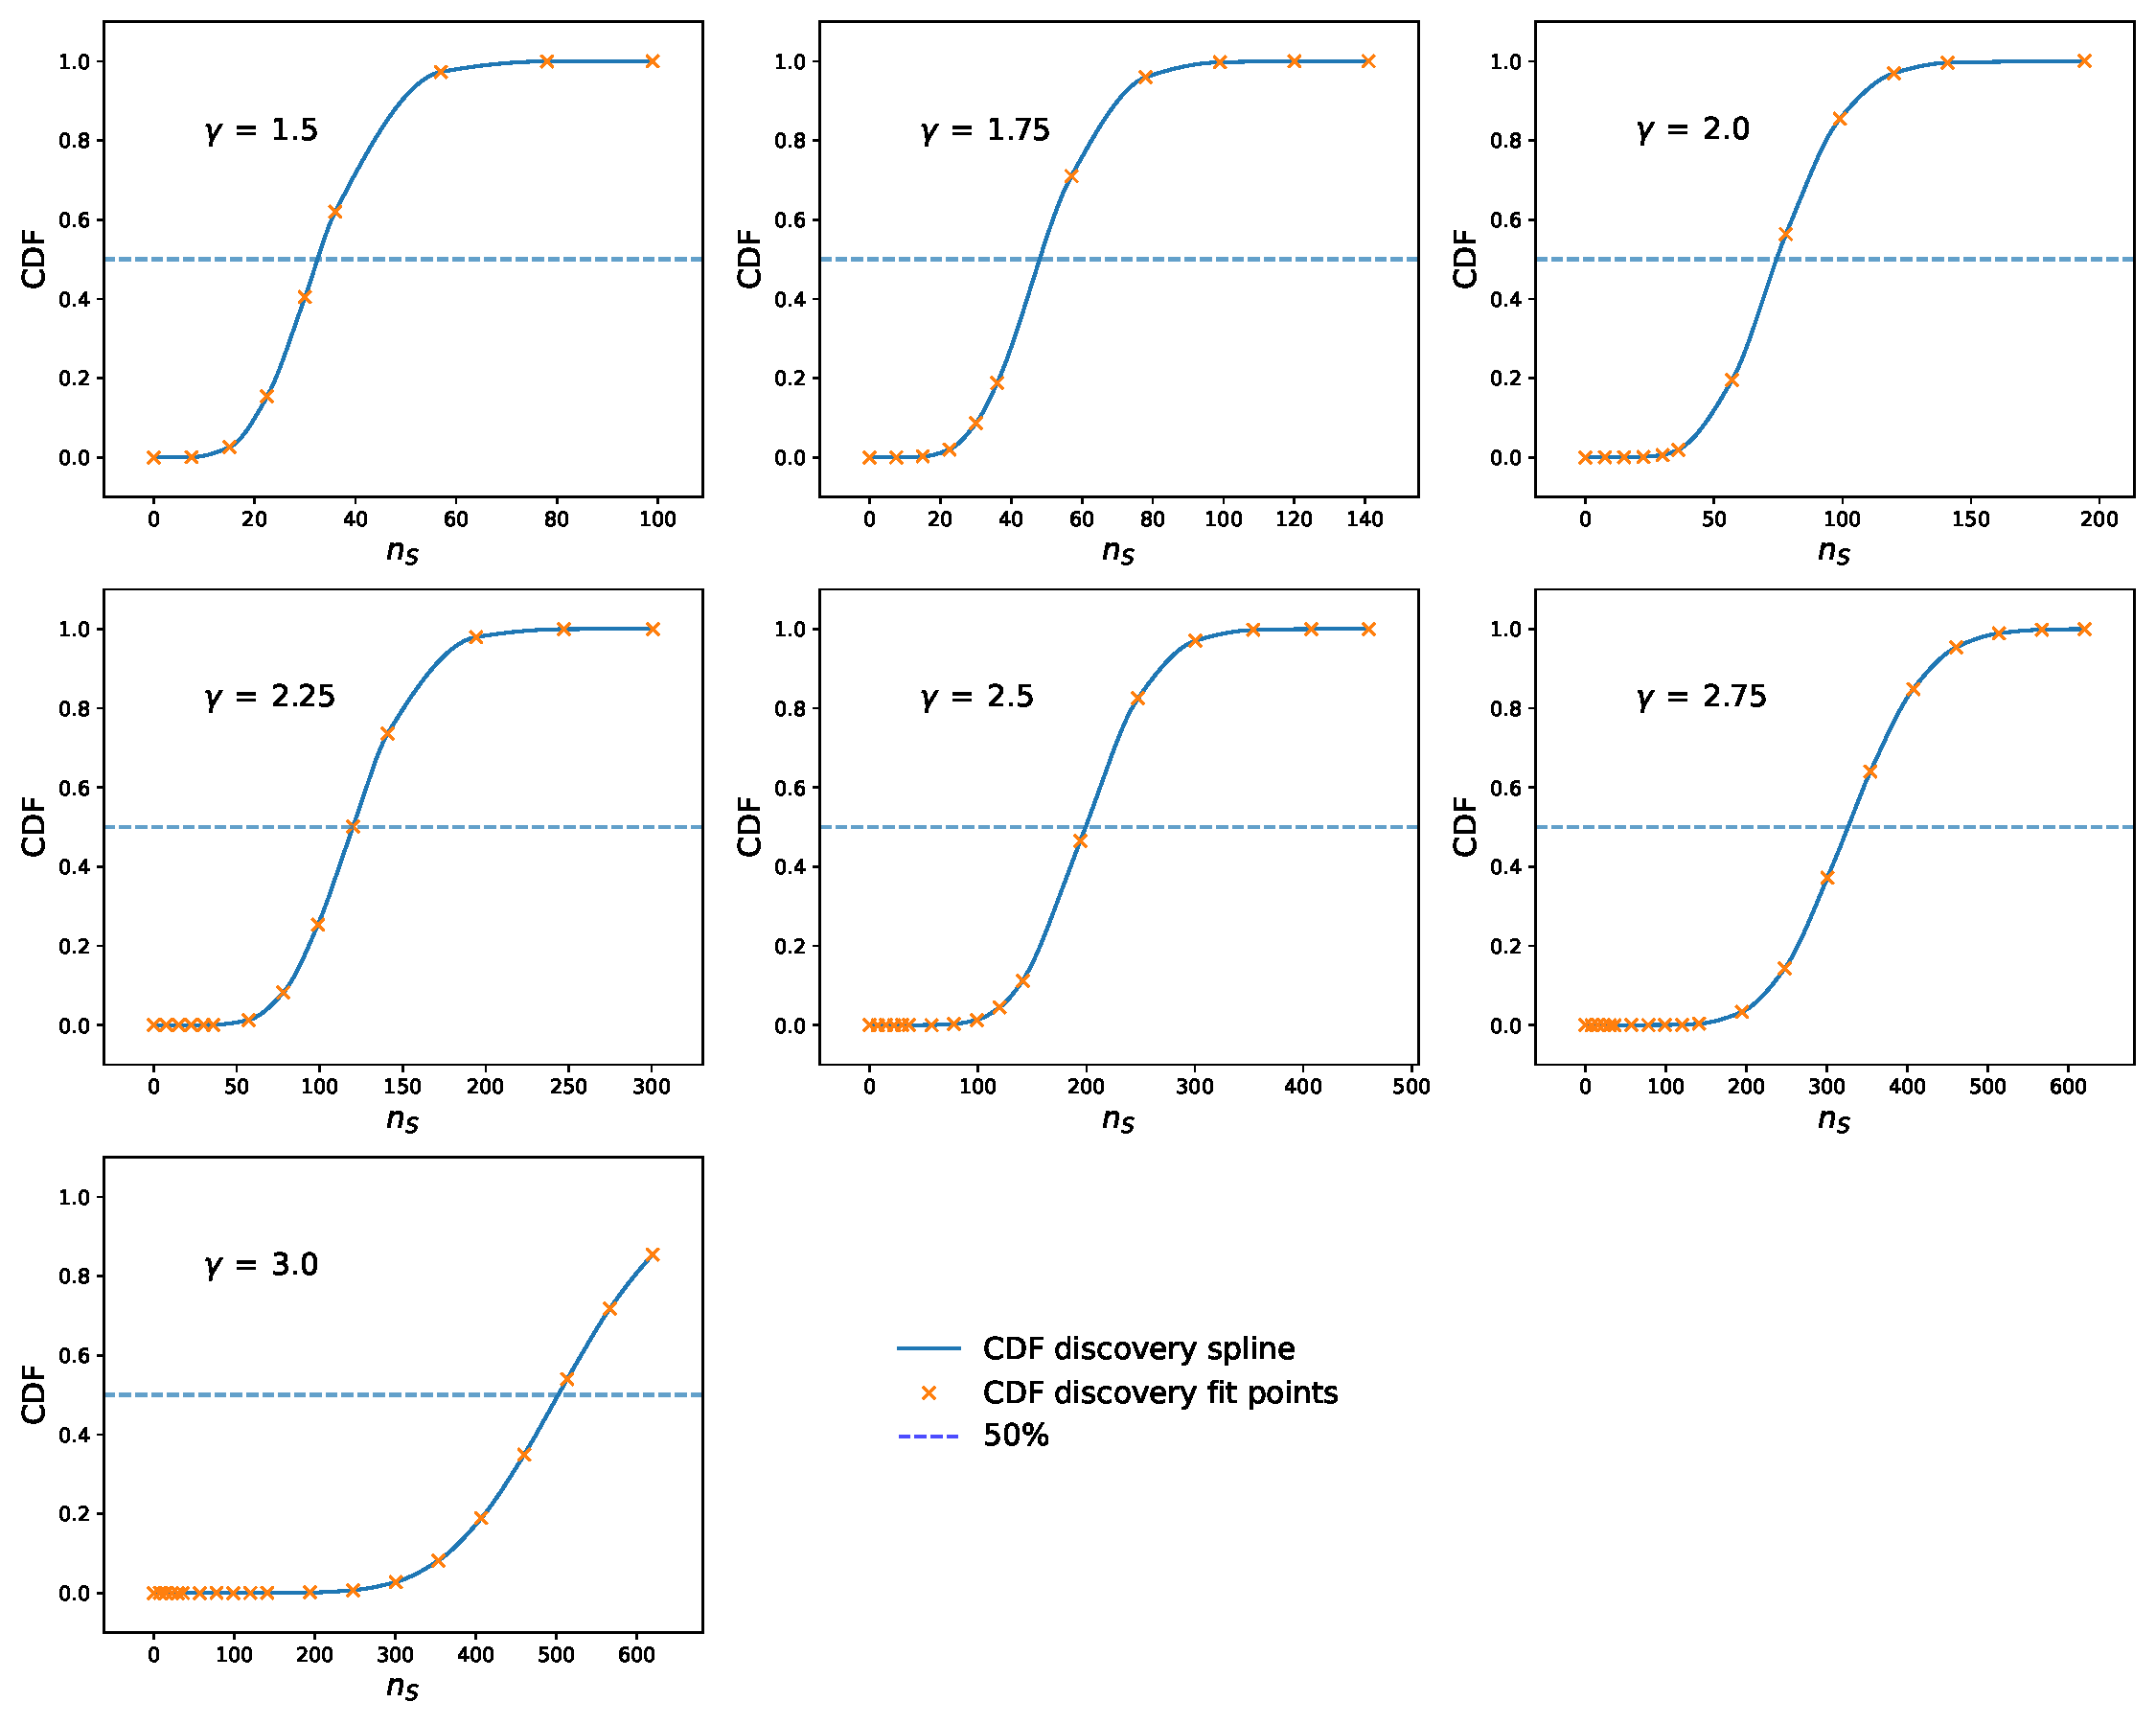
\includegraphics[width=\linewidth]{Plots/05_csky/9_years_gfu_gold_cdf_disc.pdf}
    \caption{Quantiles of the signal trials for the calculation of the discovery potential for the time integrated analysis at different spectral indices $\gamma$. A $\chi^2$ CDF fit provides a more accurate estimate of the sought signal parameter $n_\text{S}$ which satisfies the condition of the discovery potential at $\SI{50}{\percent}$.}
    \label{fig:cdf_disc}
\end{figure}
The sensitivities and discovery potentials from the CDFs can be seen in figure \ref{fig:sens_disc_time_int} and additionally in table \ref{tab:sens_disc_time_int}.
The values rise for higher spectral indices since the signal looks more background like the closer the spectral index is to $\gamma = 3$.
\begin{figure}
    \centering
    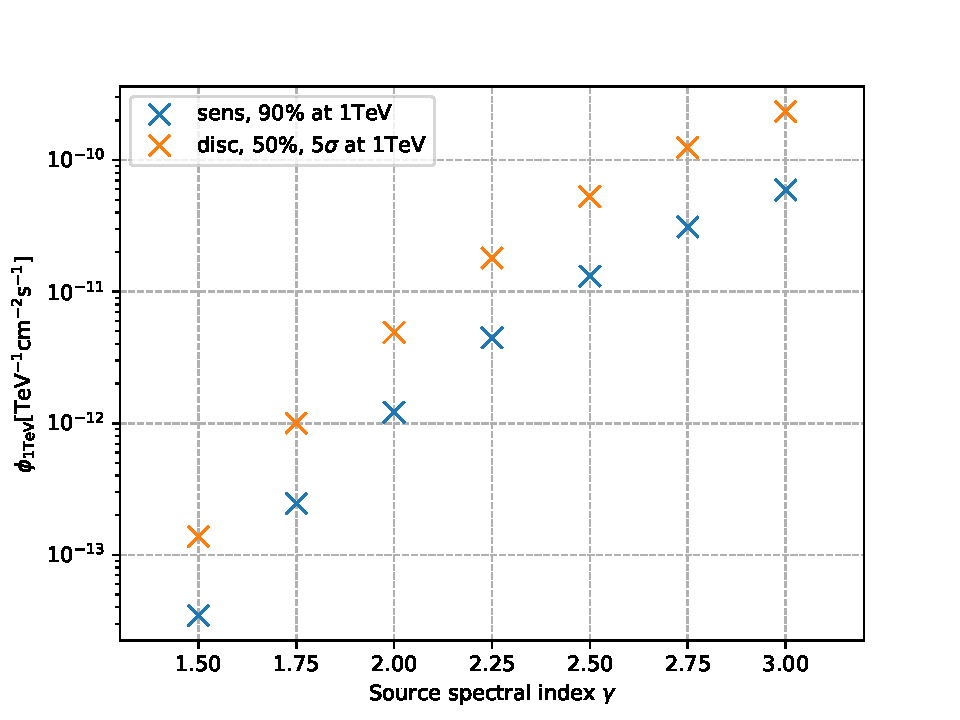
\includegraphics[width=\linewidth]{Plots/05_csky/time_int_sens_gfu_gold_9_years_new.pdf}
    \caption{Sensitivities and discovery potentials of the time integrated analysis for different spectral indices $\gamma$. The reference energy is $E_0 = \SI{1}{\tera\electronvolt}$.}
    \label{fig:sens_disc_time_int}
\end{figure}

\begin{table}
  \centering
  \caption{Sensitivities and discovery potentials for different spectral indices $\gamma$ at a reference energy of $E_0 = \SI{1}{\tera\electronvolt}$ for the time integrated analysis. Additionally the fitted number of signal events $N_\text{sig}$ satisfying the thresholds is shown.}
  \begin{tabular}{crcrc}
    \toprule
    $\gamma$ & $N_\text{sig,sens}$ &  sens in $\si{\tera\electronvolt\tothe{-1}\centi\meter\tothe{-2}\second\tothe{-1}}$ & $N_\text{sig,disc}$ & disc in $\si{\tera\electronvolt\tothe{-1}\centi\meter\tothe{-2}\second\tothe{-1}}$ \\
    \toprule
      1.50 & 8.16 & \num{3.45e-14} & 32.54 & \num{1.38e-13} \\ 1.75 & 11.86 & \num{2.46e-13} & 48.31 & \num{1.00e-12} \\ 2.00 & 18.39 & \num{1.21e-12} & 74.47 & \num{4.90e-12} \\ 2.25 & 29.65 & \num{4.46e-12} & 119.72 & \num{1.80e-11} \\ 2.50 & 49.21 & \num{1.31e-11} & 198.59 & \num{5.28e-11} \\ 2.75 & 81.12 & \num{3.10e-11} & 325.80 & \num{1.25e-10} \\ 3.00 & 127.62 & \num{5.93e-11} & 502.13 & \num{2.33e-10} \\ 
    \toprule
    \label{tab:sens_disc_time_int}
  \end{tabular}
\end{table}

\section{Examination of Fit Bias}

Several crosschecks can be made to examine the quality of the analysis results.
One of them is to check the fit of the parameters $\gamma$ and $n_\text{S}$ for bias.
The fit behaviour of the analysis can be seen in figure \ref{fig:fit_bias_gamma} for $\gamma$ and in figure \ref{fig:fit_bias_ns} for $n_\text{S}$.
The fitted spectral index is generally larger than the injected one and starts of at a spectral index of around $\hat\gamma = \num{3}$ with no injected signal events, because no signal events are equivalent to the statement that only background exists which has a spectral index of $\gamma = \num{3}$.
The larger fitted spectral index makes the analysis more conservative and therefore is not harmful for the overall results at spectral indices up to $\gamma = \num{2.5}$.
For higher spectral indices the fitted $\hat\gamma$ starts to sink below the set spectral index, since it is hard to fit for signal events that look like background. On the contrary this is harmful to the analysis results.
Equivalent behaviour can be seen for the fitted signal parameter $\hat{n}_\text{S}$.
\begin{figure}
    \centering
    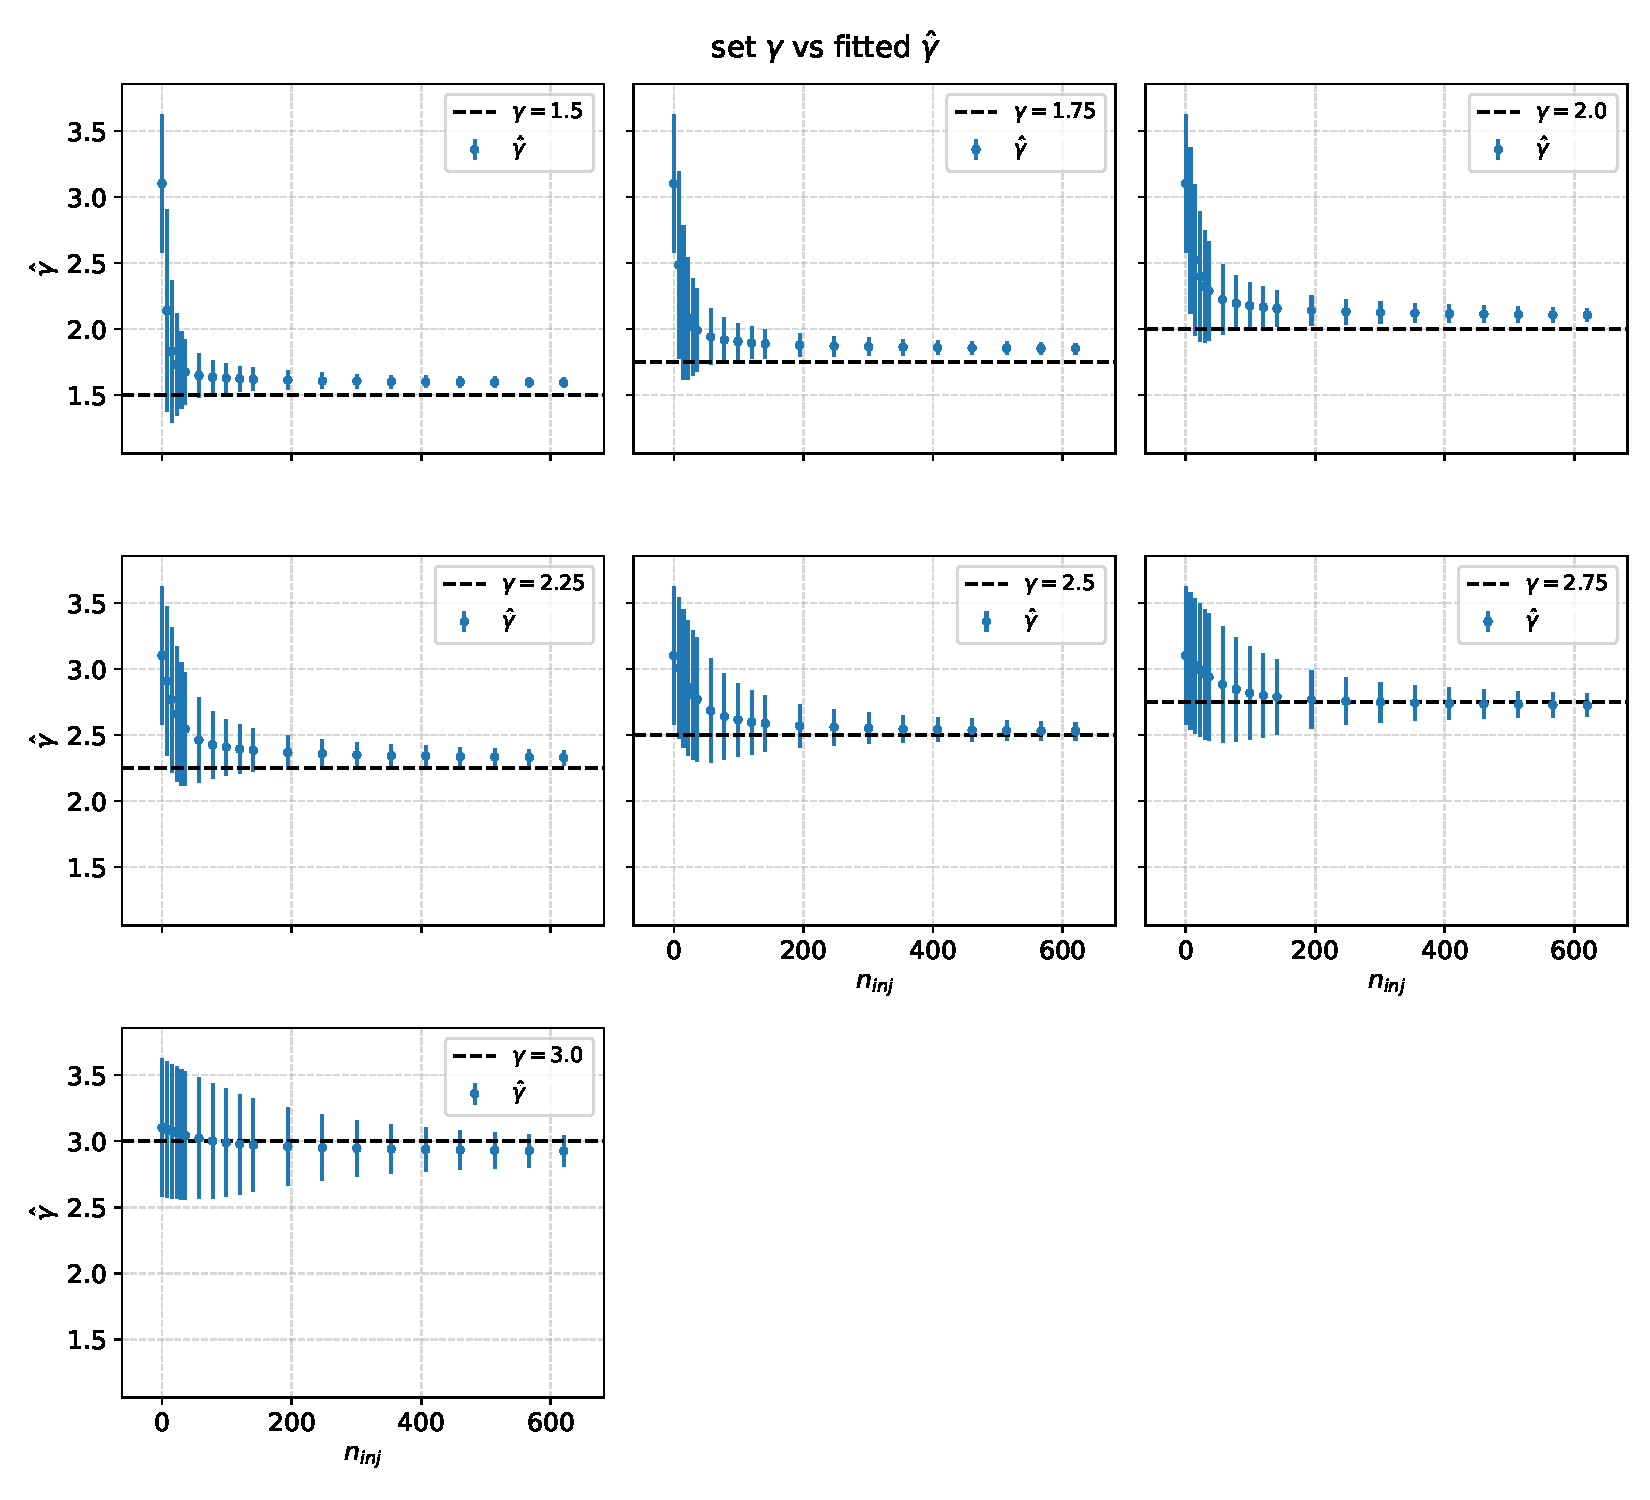
\includegraphics[width=\linewidth]{Plots/05_csky/gamma_fit_auto_3.pdf}
    \caption{Fitted spectral index $\hat\gamma$ in dependence of the injected number of signal events $n_\text{inj}$ with spectral index $\gamma$, shown with a horizontal black dashed line, for the trials used in the time integrated analysis.}
    \label{fig:fit_bias_gamma}
\end{figure}

\begin{figure}
    \centering
    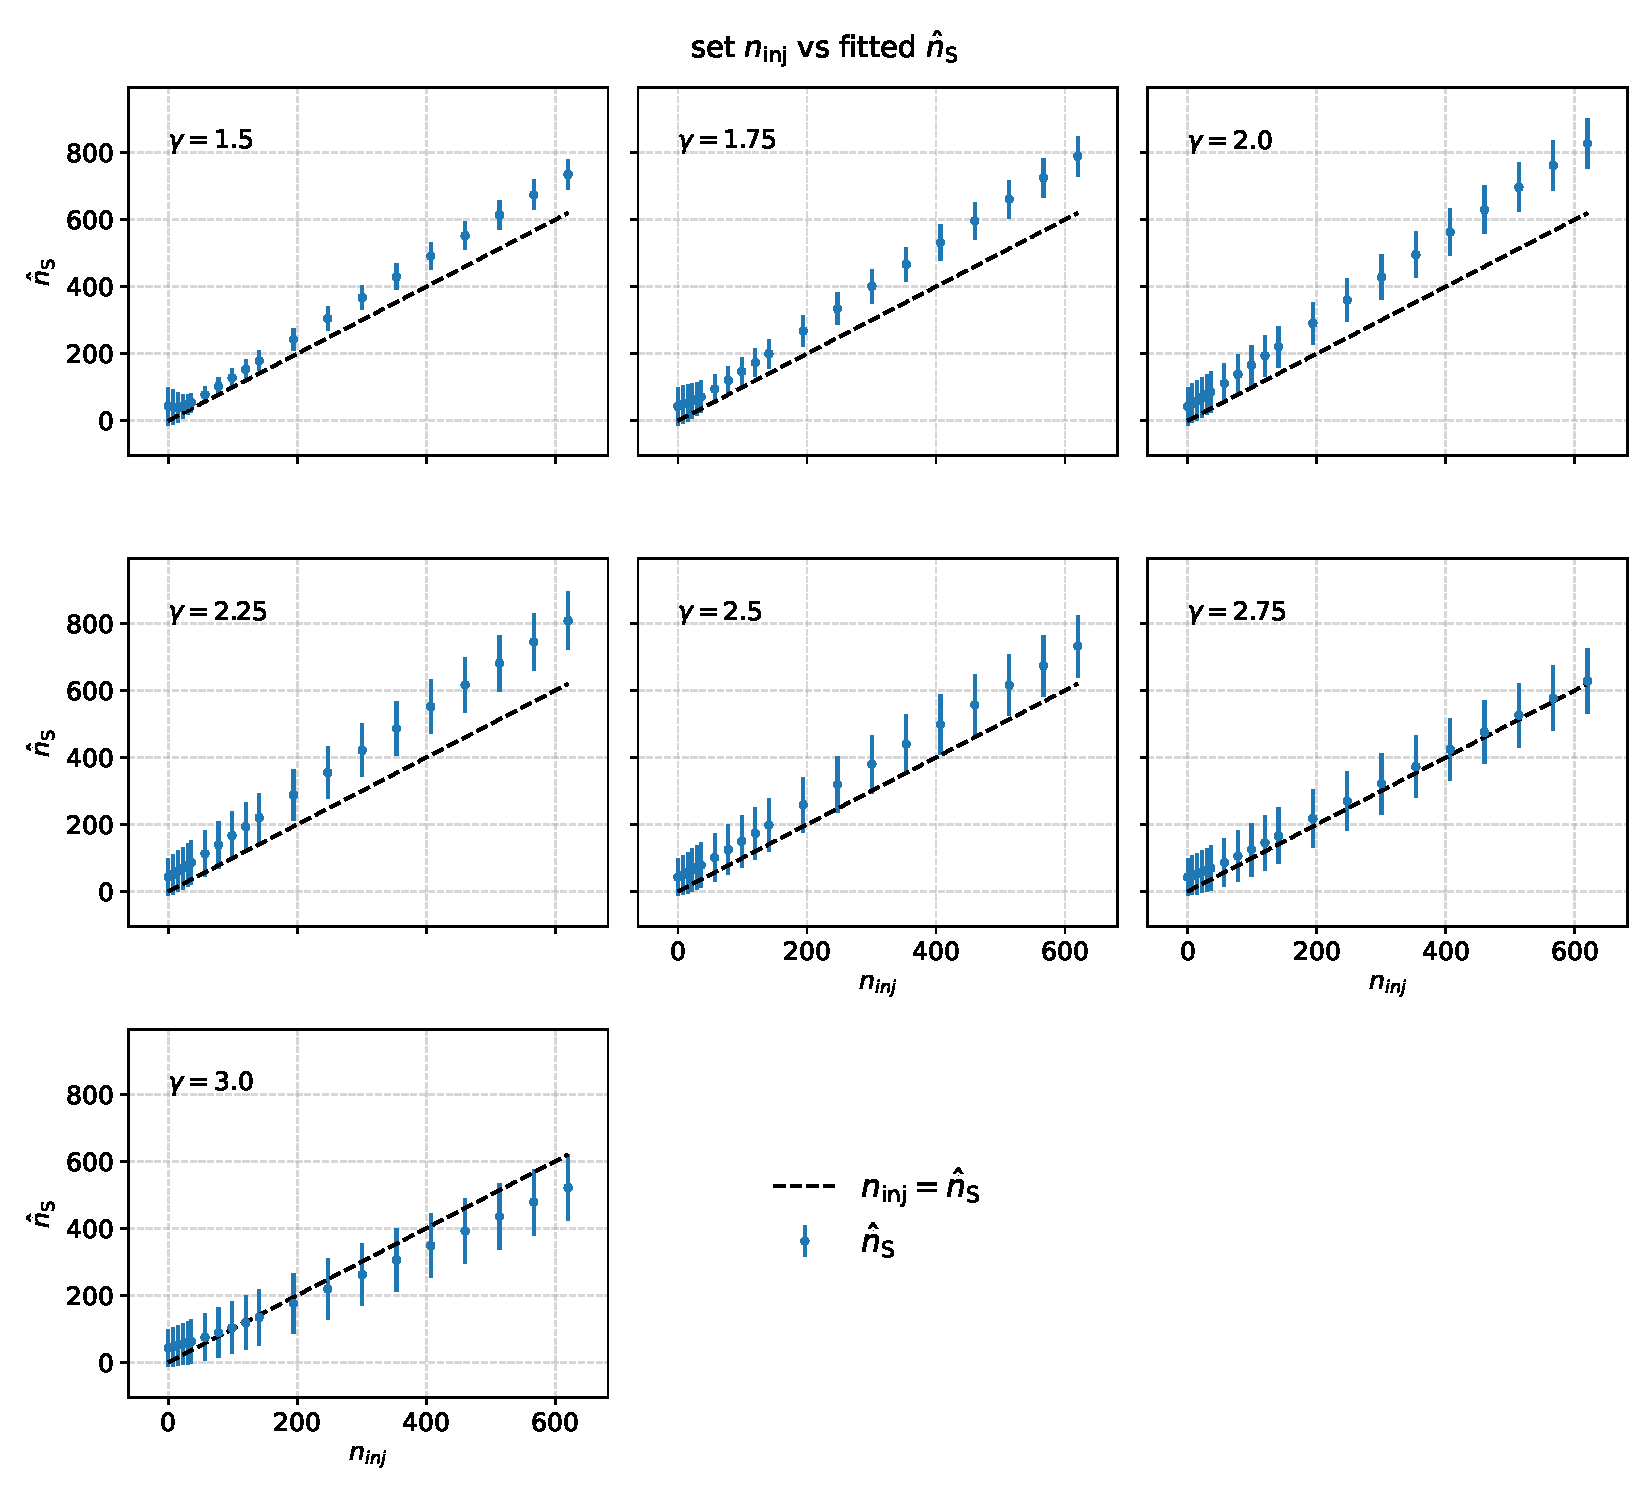
\includegraphics[width=\linewidth]{Plots/05_csky/ns_fit_auto_4.pdf}
    \caption{Fitted number of signal events $\hat{n}_{\text{S}}$ in dependence of the injected number of signal events $n_\text{inj}$ with spectral index $\gamma$ for the time integrated analysis. The black dashed line shows the equality of fitted and injected number of signal events.}
    \label{fig:fit_bias_ns}
\end{figure}

\chapter{Time-Dependent Search} \label{sec:csky_time_dep}

The time-dependent search examines $\num{10}$ sources independently of each other.
Ideally, all gfu-gold alerts should be examined and, in addition, preferably stacked.
However, time-dependent stacking is not yet sufficiently implemented in csky during the development of this thesis, and examining all sources individually would require too much computing capacity.
Chapter \ref{sec:tdepps} contains more detailed information on the technical details of time-dependent stacking.
Therefore, only the $\num{10}$ alerts with the highest signalness in the set are used as sources.
These can be seen in table \ref{tab:sources_time_dep}.

\section{Background Trials}

The background trials for all $\num{10}$ sources can be seen in figure \ref{fig:bg_trials_time_dep}.
Since the length $dt$ of the time windows is fitted, the number of degrees of freedom is generally greater than in the time integrated analysis.
The $\chi^2$ distribution generated via the trials is thus somewhat more convex.
The values to calculate the fluences can be seen in table \ref{tab:sigma_time_dep}.
In addition to the test statistics values, the time windows of the background trials can be examined.
These are shown in figure \ref{fig:bg_trials_time_dep_time_windows}.
The shape of the time window distribution results from the fact that the time window prior prefers larger time windows, while the data allows for several shorter flares.
Therefore, there are more short time windows, fewer in the middle range, and again more closing in at the maximum time window limit of $\num{200}$ days.
This behaviour can be additionally observed in figure \ref{fig:bg_trials_time_dep_time_windows_ns}, showing the fitted signal parameter $\hat{n}_\text{sig}$ in dependence of the fitted time window length $dt$.
Larger timewindows allow for more potential signal events.
Generally a time window gets defined by the temporal space between $\num{2}$ events, which means a time window already consists of at least $\num{2}$ events.
However, this does not mean the fitted value of the signal parameter is atleast $2$, but it explains why the majority of trials are above a signal parameter of zero, especially for extremely short time windows.
Altogether, many possible numbers of signal events are represented in the background trials, but most of them are logically in the lower range.
\begin{figure}
    \centering
    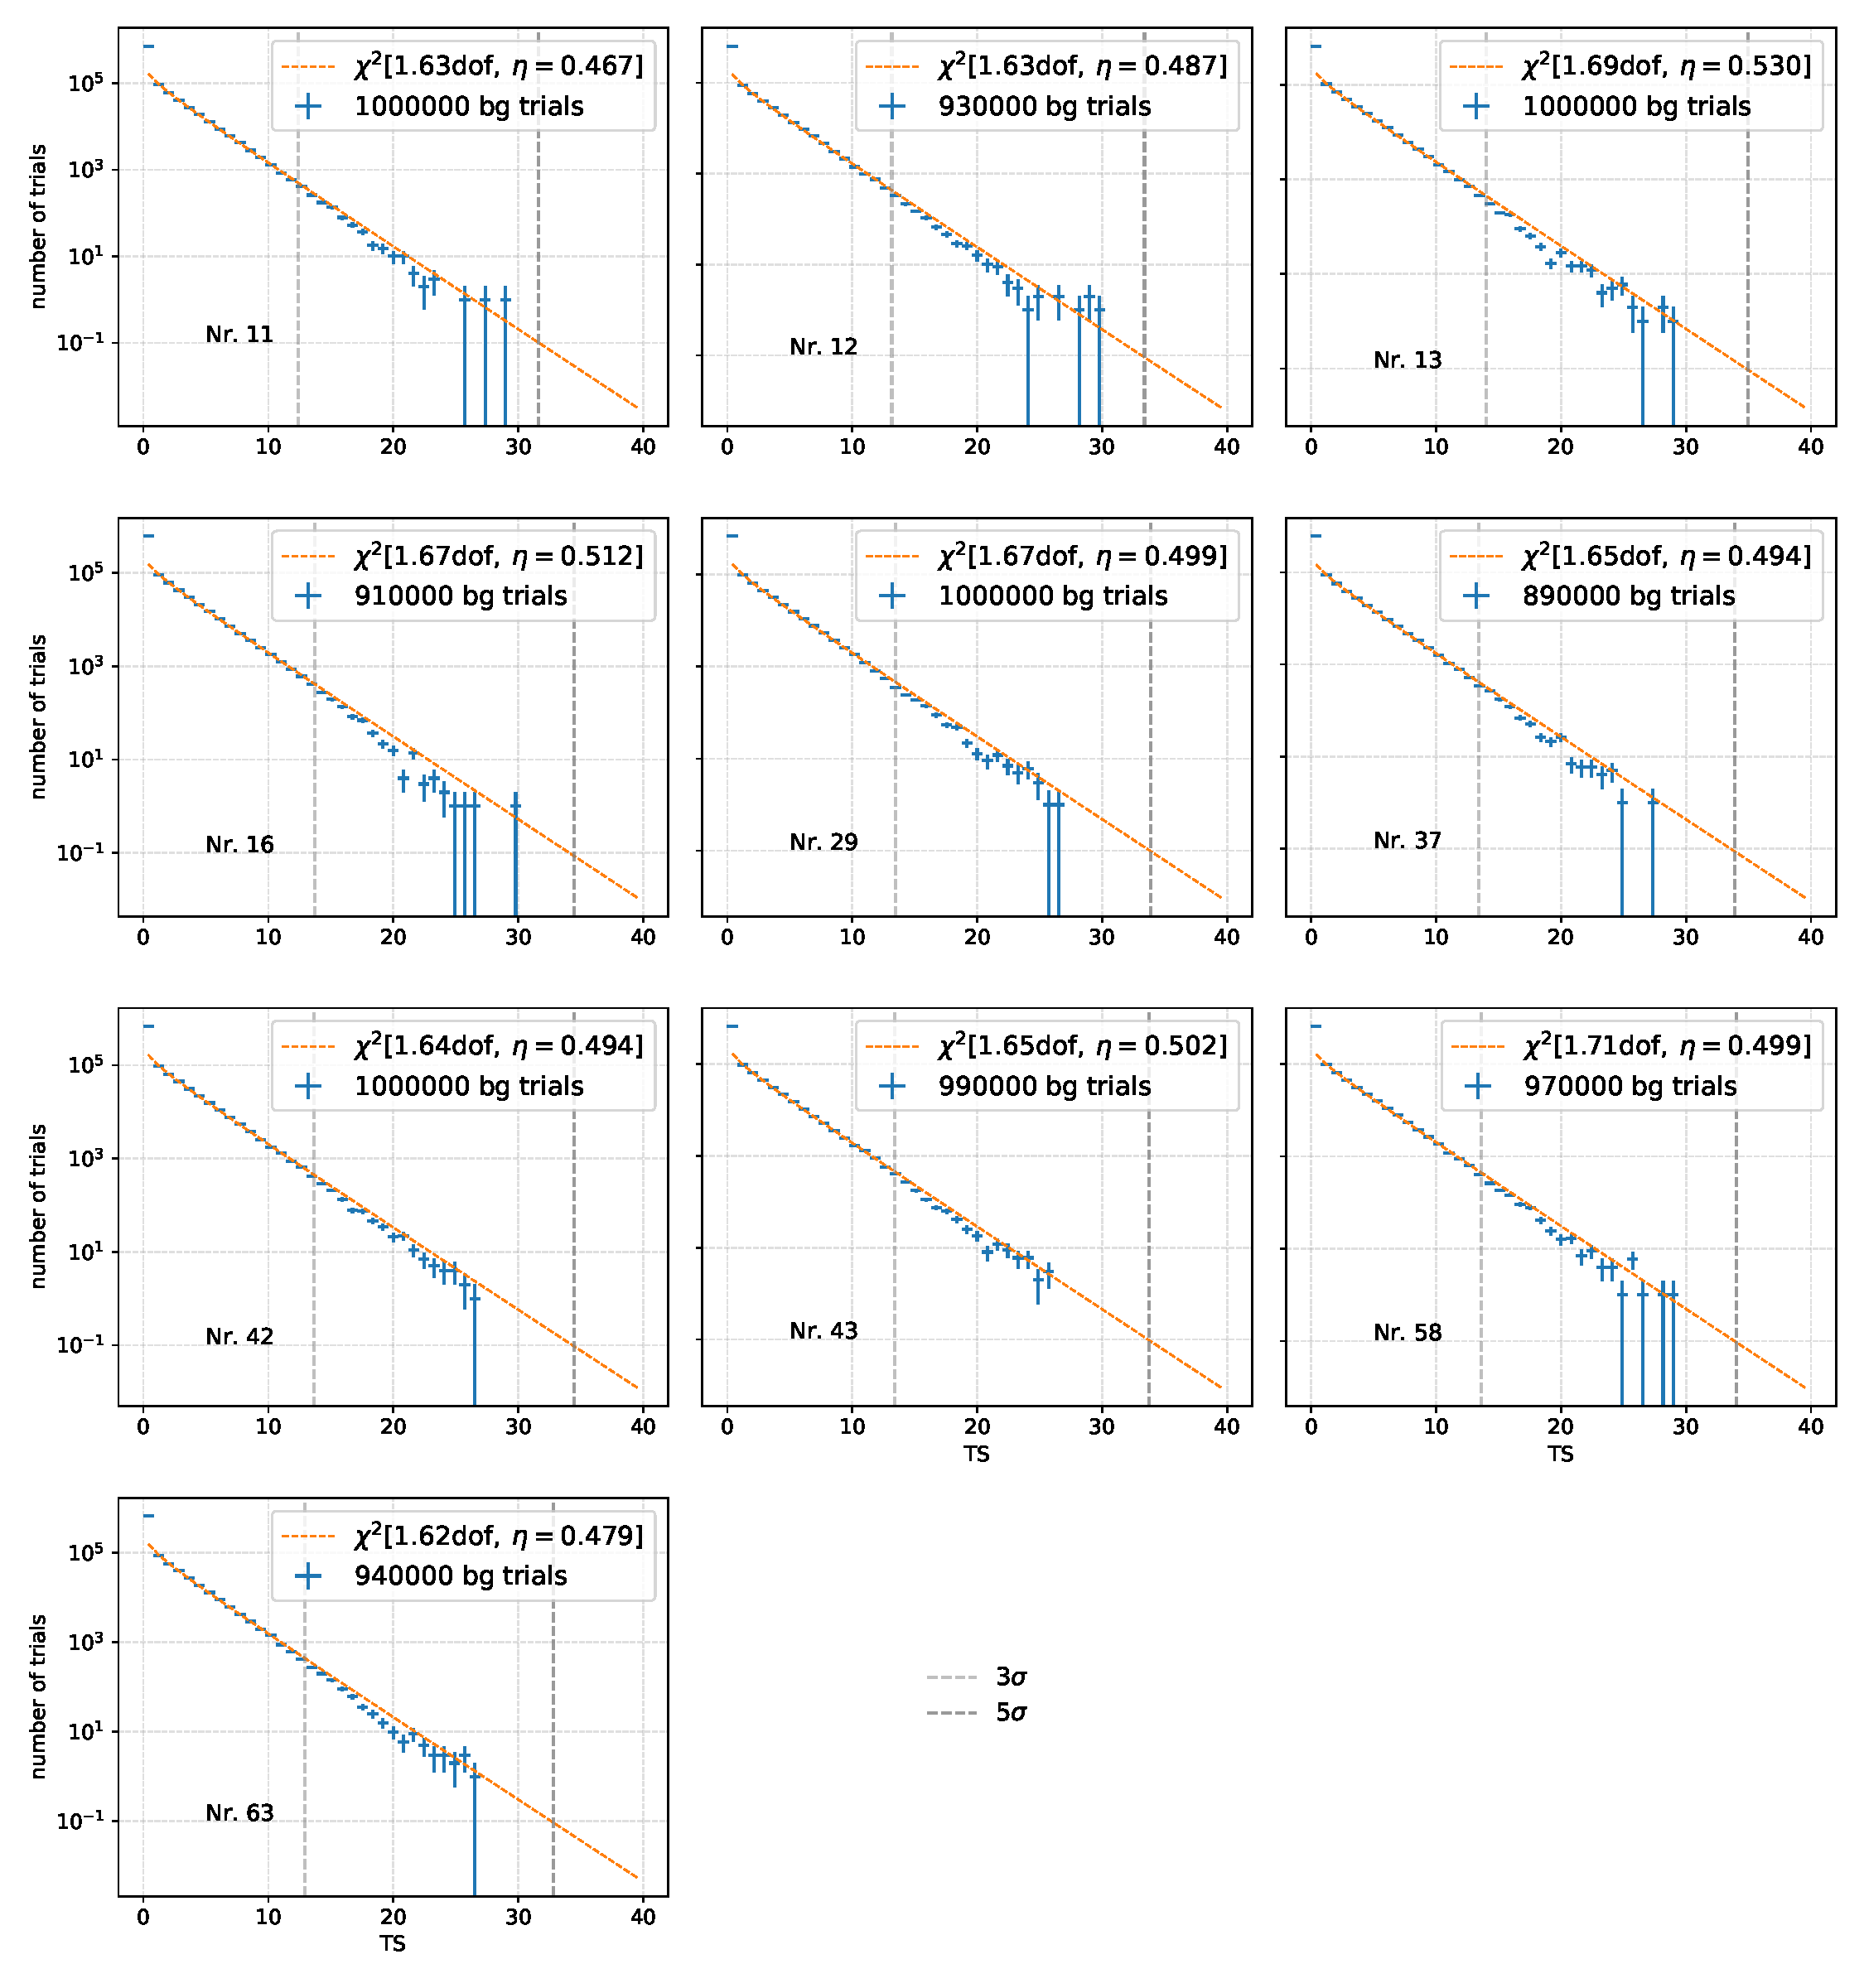
\includegraphics[width=\linewidth]{Plots/05_csky/9_years_gfu_gold_time_dep_bg_t0.pdf}
    \caption{Histograms of the background test statistic values for all $\num{10}$ sources used in the time-dependent analysis. Shown are also the number of degrees of freedom $dof$ and the ratio of positive and negative values $\eta$. The id of the sources corresponds to table \ref{tab:sources} or \ref{tab:sources_time_dep} respectively.}
    \label{fig:bg_trials_time_dep}
\end{figure}
\begin{table}
  \centering
  \caption[]{Table of number of trials, degrees of freedom $dof$, symmetry parameter $\eta$, median\footnotemark, $\num{3}\sigma$ and $\num{5}\sigma$ values of the background test statistics for the time-dependent analysis for all $\num{10}$ sources seen in figure \ref{fig:bg_trials_time_dep}.}
  \begin{tabular}{crccccc}
    \toprule
    Nr. & trials & $dof$ & $\eta$ & median & $\num{3}\sigma$ & $\num{5}\sigma$ \\
    \toprule
      11 & 0.000 & 12.413 & 31.600 \\ 12 & 0.000 & 13.171 & 33.390 \\ 13 & 0.079 & 14.013 & 34.950 \\ 16 & 0.030 & 13.735 & 34.461 \\ 29 & 0.000 & 13.471 & 33.910 \\ 37 & 0.000 & 13.436 & 33.919 \\ 42 & 0.000 & 13.642 & 34.476 \\ 43 & 0.005 & 13.395 & 33.752 \\ 58 & 0.000 & 13.587 & 34.041 \\ 63 & 0.000 & 12.909 & 32.821 \\ 
    \toprule
    \label{tab:sigma_time_dep}
  \end{tabular}
\end{table}
\footnotetext{Some median values are very close to if not $\num{0}$.}
\begin{figure}
    \centering
    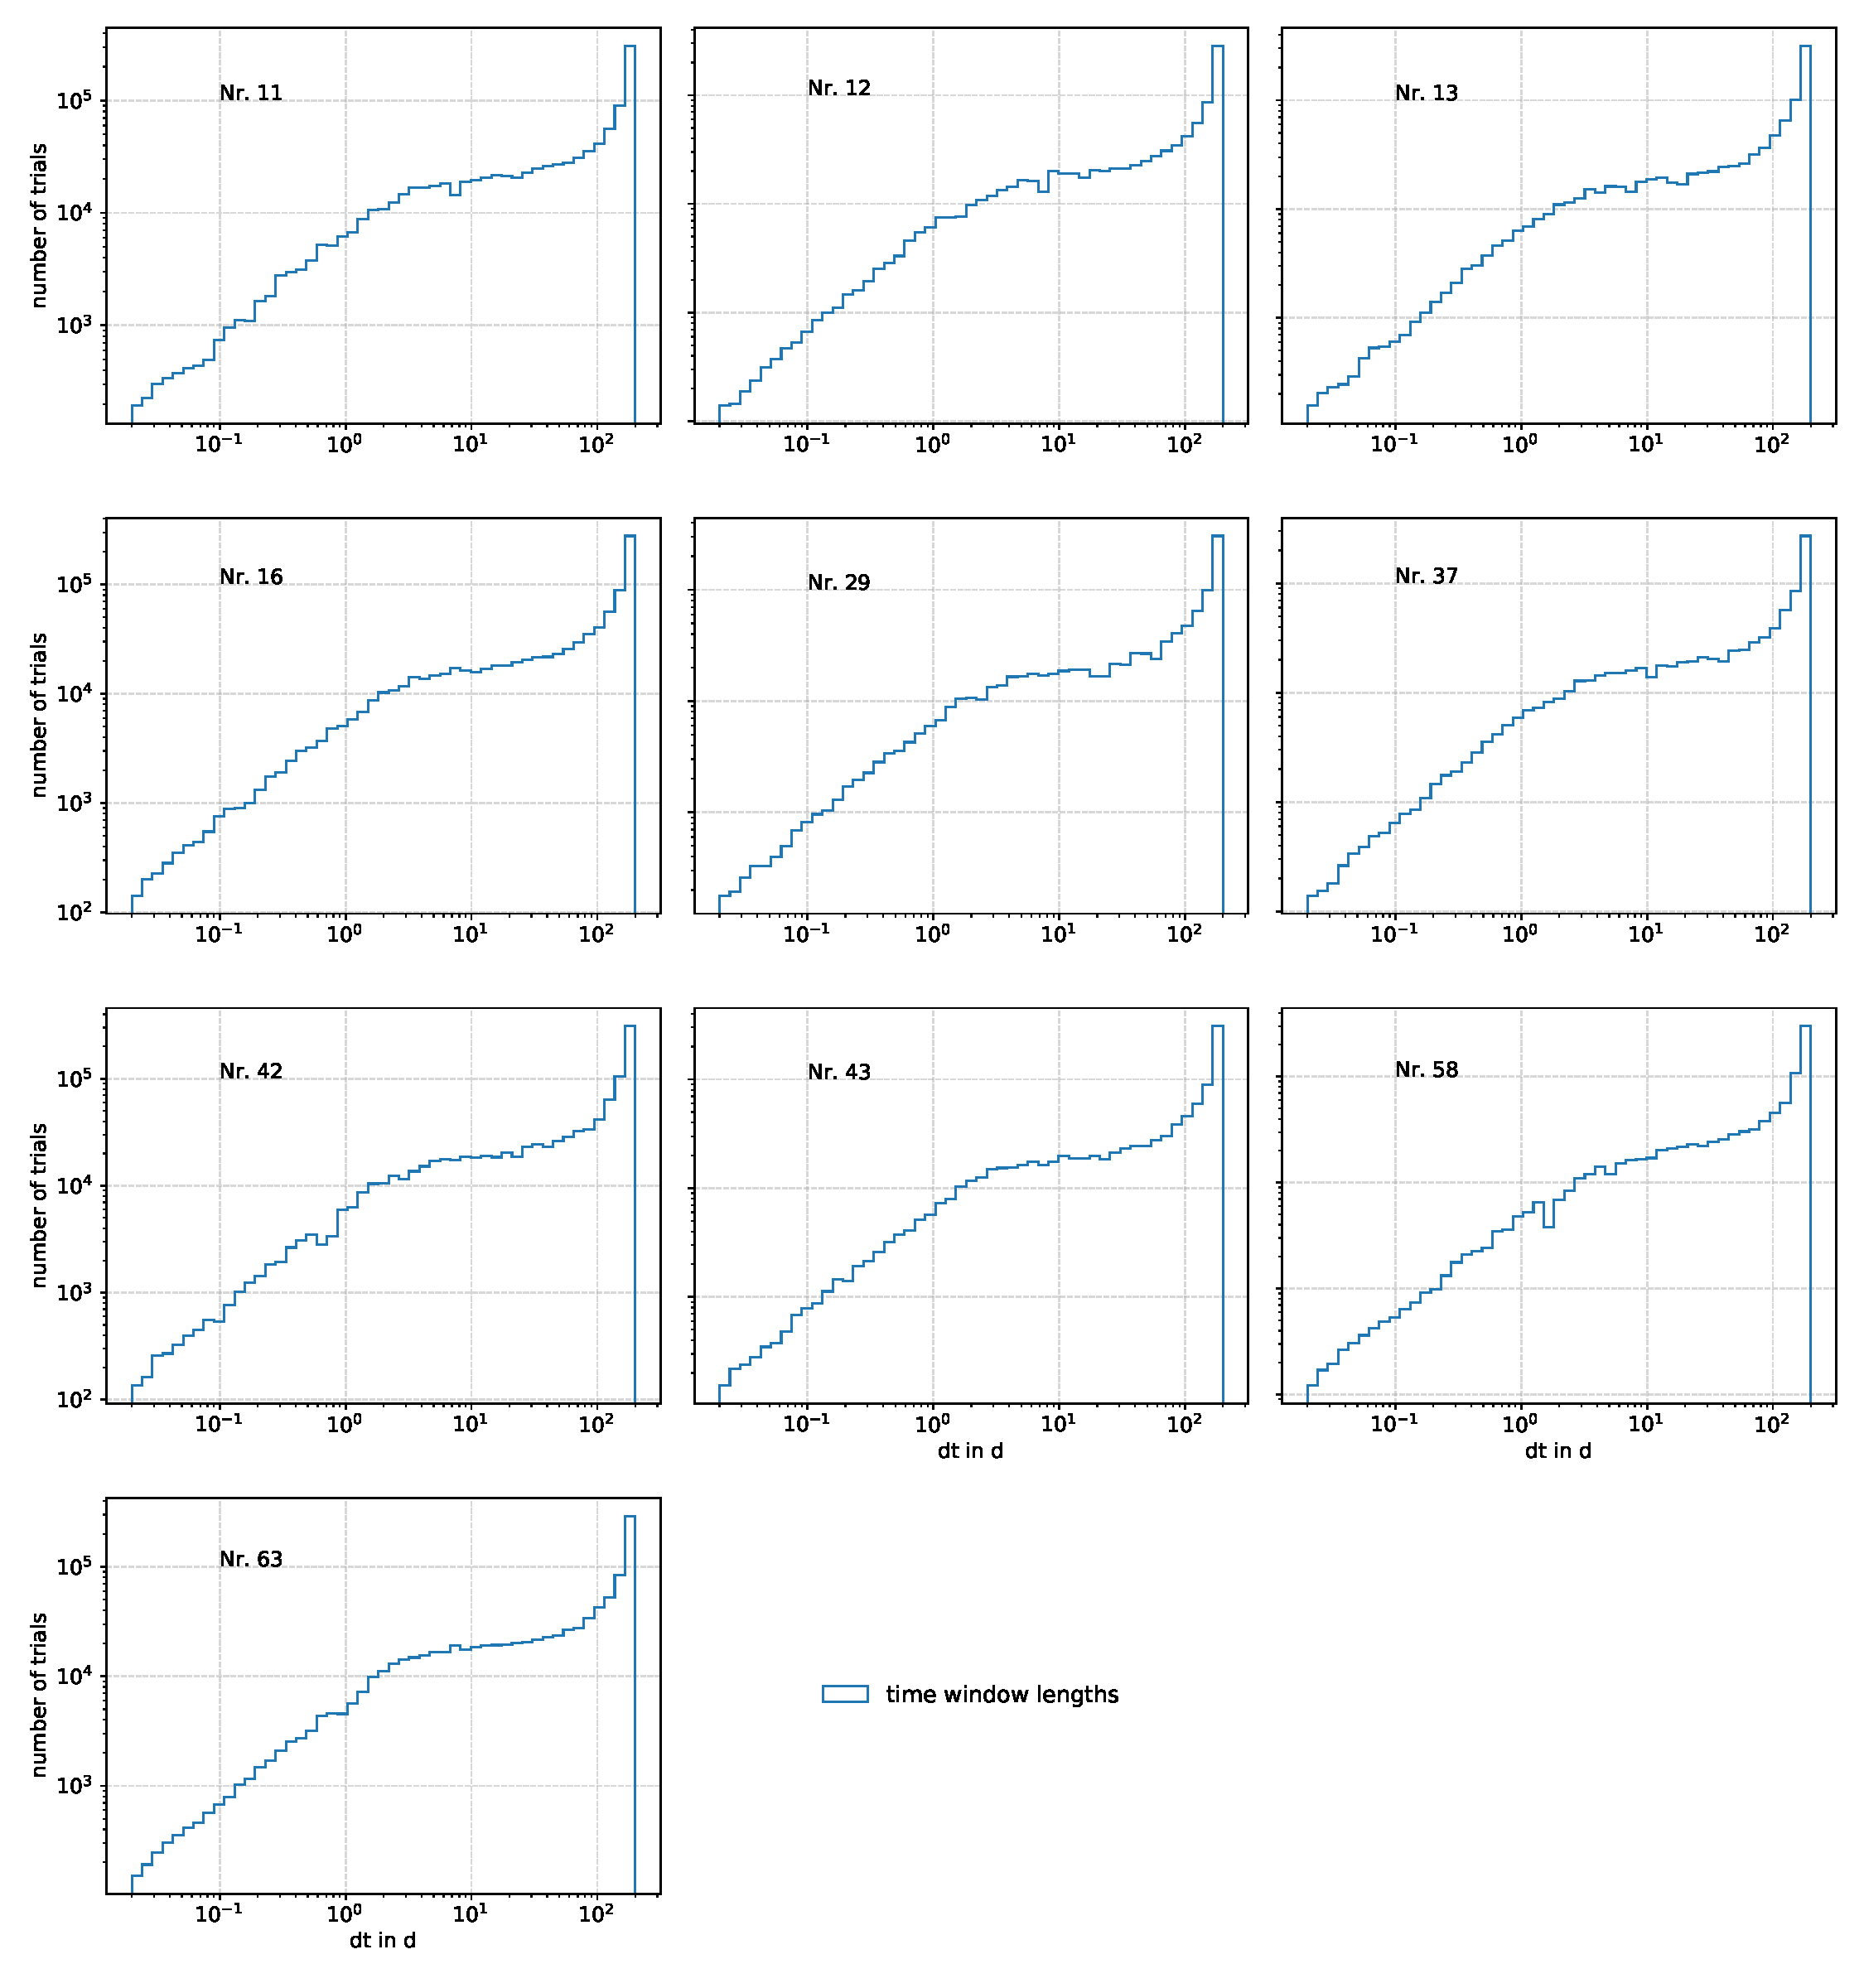
\includegraphics[width=\linewidth]{Plots/05_csky/9_years_gfu_gold_time_dep_bg_dt.pdf}
    \caption{Histograms of the background time window lengths $dt$ in days of all $\num{10}$ sources for the time-dependent analysis.}
    \label{fig:bg_trials_time_dep_time_windows}
\end{figure}
\begin{figure}
    \centering
    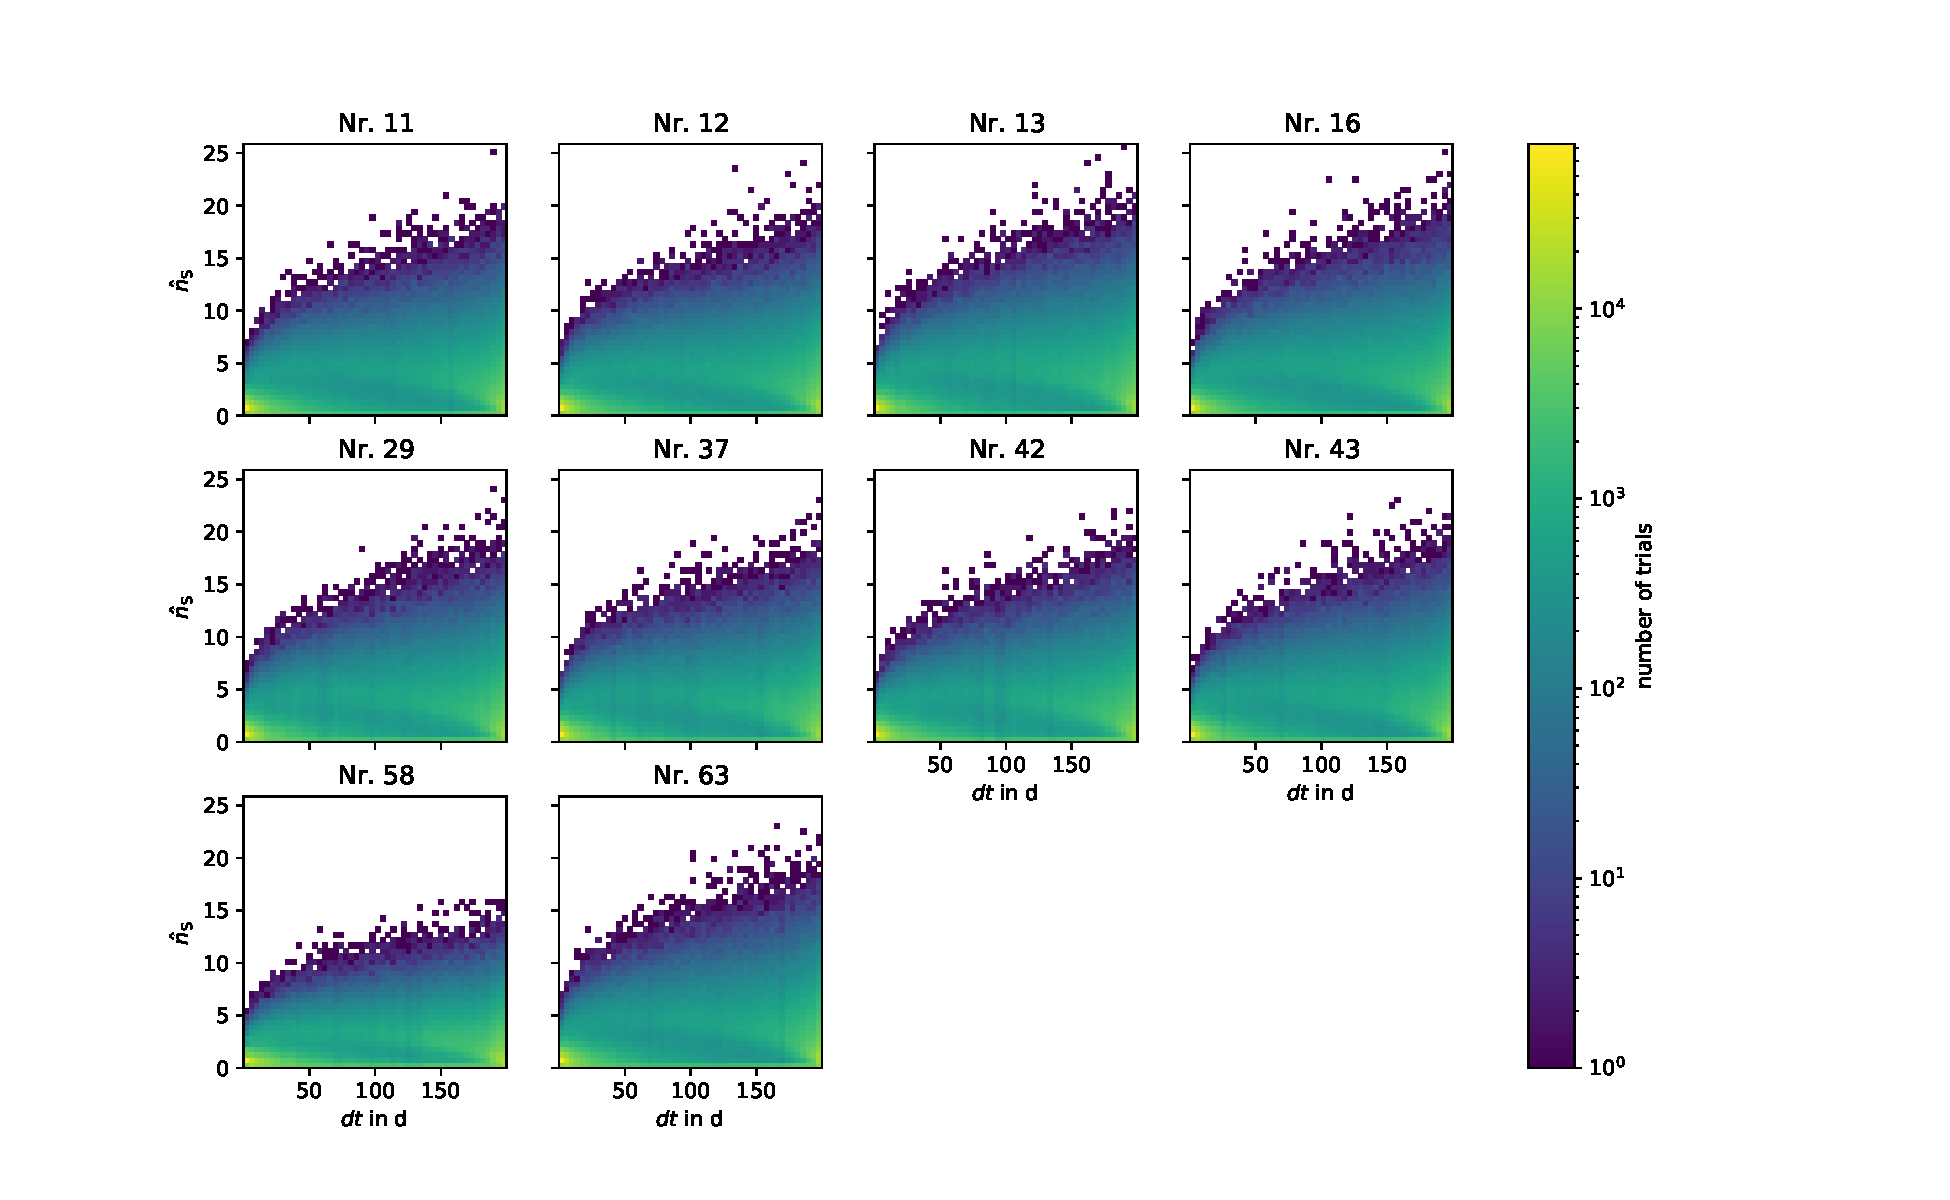
\includegraphics[width=\linewidth]{Plots/05_csky/time_window_ns_bg_time_dep.pdf}
    \caption{Histograms of the fitted number of signal events $\hat{n}_\text{S}$ in dependence of the time window lengths $dt$ in days of the background trials for the time-dependent analysis for all $\num{10}$ sources.}
    \label{fig:bg_trials_time_dep_time_windows_ns}
\end{figure}

\section{Signal Trials}

\begin{figure}
    \centering
    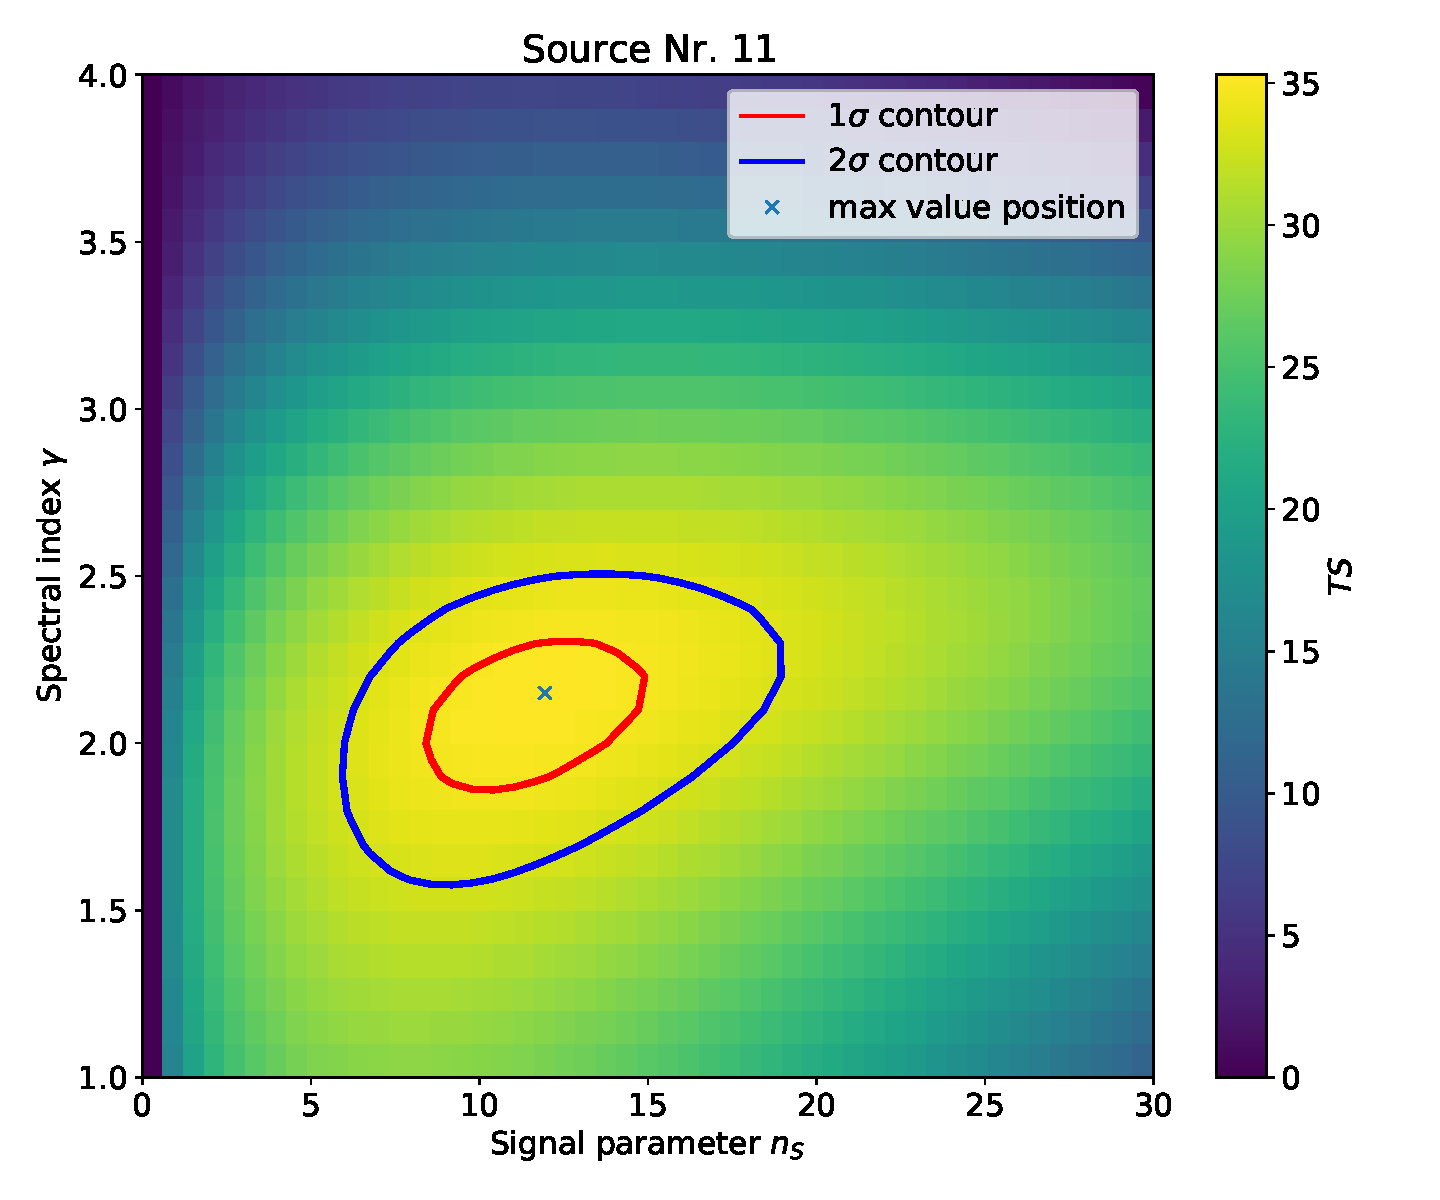
\includegraphics[width=\linewidth]{Plots/05_csky/llh_scan_1.pdf}
    \caption{Scan of the likelihoodspace for source number $\num{11}$ with a timewindow of $\SI{200}{\day}$ for the time-dependent analysis. The scan is in the spectral index $\gamma$ and the signal parameter $n_\text{S}$. The number of induced signal events is $n_S = \num{10}$ with a spectral index of $\gamma = 2$. The maximum test statistic value is marked in the plot including the contours of $\num{1}\sigma$ and $\num{2}\sigma$ and source number corresponds to table \ref{tab:sources}.}
    \label{fig:llh_scan_time_dep}
\end{figure}

\begin{figure}
    \centering
    \includegraphics[width=\linewidth]{Plots/05_csky/9_years_gfu_gold_time_dep_cdf_sens.pdf}
    \caption{Quantiles of the signal trials for the calculation of the sensitivity for the time-dependent analysis of all $\num{10}$ sources at a spectral index of $\gamma=\num{2}$. A $\chi^2$ CDF fit provides a more accurate estimate of the sought signal parameter $n_\text{S}$ which satisfies the condition of the sensitivity at $\SI{90}{\percent}$ represented via a dashed line.}
    \label{fig:time_dep_cdf_sens}
\end{figure}

\begin{figure}
    \centering
    \includegraphics[width=\linewidth]{Plots/05_csky/9_years_gfu_gold_time_dep_cdf_disc.pdf}
    \caption{Quantiles of the signal trials for the calculation of the discovery potential for the time-dependent analysis of all $\num{10}$ sources at a spectral index of $\gamma=\num{2}$. A $\chi^2$ CDF fit provides a more accurate estimate of the sought signal parameter $n_\text{S}$ which satisfies the condition of the discovery potential at $\SI{50}{\percent}$ represented via a dashed line.}
    \label{fig:time_dep_cdf_disc}
\end{figure}

\begin{figure}
    \centering
    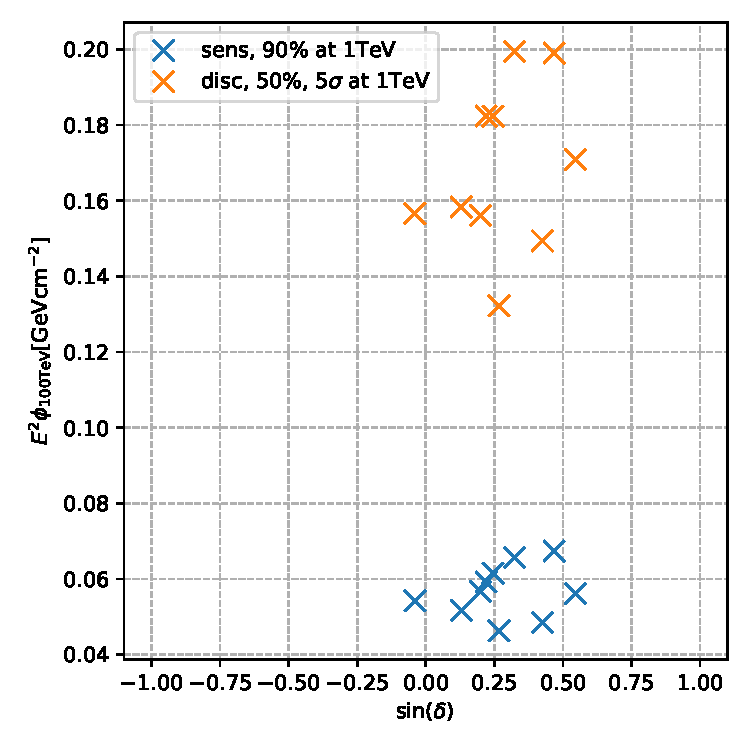
\includegraphics[width=10cm]{Plots/05_csky/time_dep_sens_disc_dec.pdf}
    \caption{Sensitivities and discovery potentials for all $\num{10}$ sources in dependece of their position at a reference energy of $E_0 = \SI{1}{\tera\electronvolt}$ for the time-dependend analysis.}
    \label{fig:sens_disc_time_dep}
\end{figure}

\begin{table}
  \centering
  \caption{Sensitivities and discovery potentials for different sources at a reference energy of $E_0 = \SI{1}{\tera\electronvolt}$ and a spectral index $\gamma=2$ for the time-dependent analysis. Additionally the fitted number of signal events $N_\text{sig}$ satisfying the thresholds is shown.}
  \begin{tabular}{crcrc}
    \toprule
    Nr. & $N_\text{sig,sens}$ &  sens in $\si{\giga\electronvolt\centi\meter\tothe{-2}}$ & $N_\text{sig,disc}$ & disc in $\si{\giga\electronvolt\centi\meter\tothe{-2}}$ \\
    \toprule
      11 & 0.199 & 3.10 & \num{5.67e-2} & 8.53 & \num{1.56e-1} \\ 12 & 0.245 & 3.04 & \num{6.15e-2} & 9.01 & \num{1.82e-1} \\ 13 & 0.425 & 2.83 & \num{4.85e-2} & 8.71 & \num{1.49e-1} \\ 16 & 0.129 & 2.91 & \num{5.17e-2} & 8.91 & \num{1.58e-1} \\ 29 & 0.220 & 2.87 & \num{5.93e-2} & 8.84 & \num{1.82e-1} \\ 37 & 0.324 & 2.95 & \num{6.57e-2} & 8.94 & \num{1.99e-1} \\ 42 & 0.468 & 2.99 & \num{6.74e-2} & 8.84 & \num{1.99e-1} \\ 43 & 0.545 & 2.97 & \num{5.61e-2} & 9.03 & \num{1.71e-1} \\ 58 & 0.267 & 2.33 & \num{4.63e-2} & 6.65 & \num{1.32e-1} \\ 63 & -0.040 & 3.01 & \num{5.43e-2} & 8.69 & \num{1.57e-1} \\ 
    \toprule
    \label{tab:sens_disc_time_dep}
  \end{tabular}
\end{table}

\begin{figure}
    \centering
    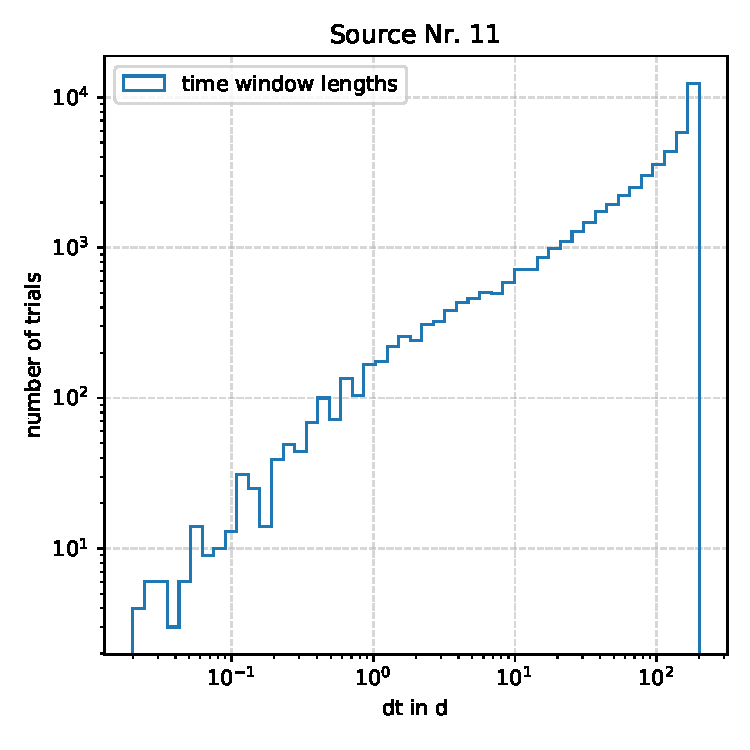
\includegraphics[width=\linewidth]{Plots/05_csky/9_years_gfu_gold_time_dep_sens_dt_1.pdf}
    \caption{Histogram of the time window lengths $dt$ in days of source number $\num{11}$ for the time-dependent analysis for the set of signal trials with the number of injected signal events closest to satisfying the condition to calculate the sensitivity.}
    \label{fig:sens_dt}
\end{figure}

\begin{figure}
    \centering
    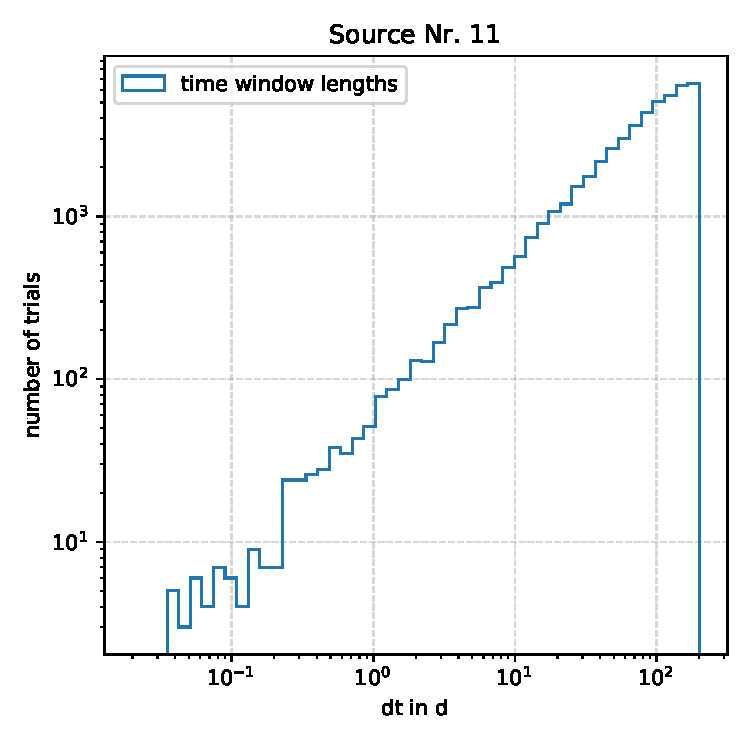
\includegraphics[width=\linewidth]{Plots/05_csky/9_years_gfu_gold_time_dep_disc_dt_1.pdf}
    \caption{Histogram of the time window lengths $dt$ in days of source number $\num{11}$ for the time-dependent analysis for the set of signal trials with the number of injected signal events closest to satisfying the condition to calculate the discovery potential.}
    \label{fig:disc_dt}
\end{figure}

\begin{figure}
    \centering
    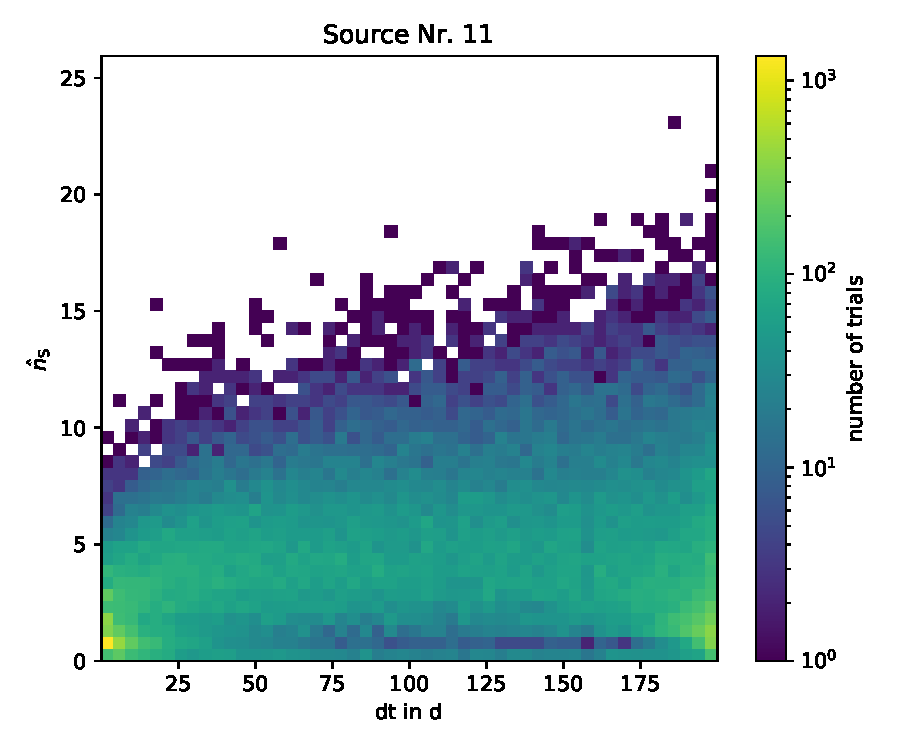
\includegraphics[width=\linewidth]{Plots/05_csky/time_windows_ns_sens_time_dep_1.pdf}
    \caption{Histogram of the time window lengths $dt$ in days in dependence of the fitted signal parameter $\hat{n}_\text{S}$ of source number $\num{11}$ for the time-dependent analysis for the set of signal trials with the number of injected signal events closest to satisfying the condition to calculate the sensitivity.}
    \label{fig:sens_ns_dt}
\end{figure}

\begin{figure}
    \centering
    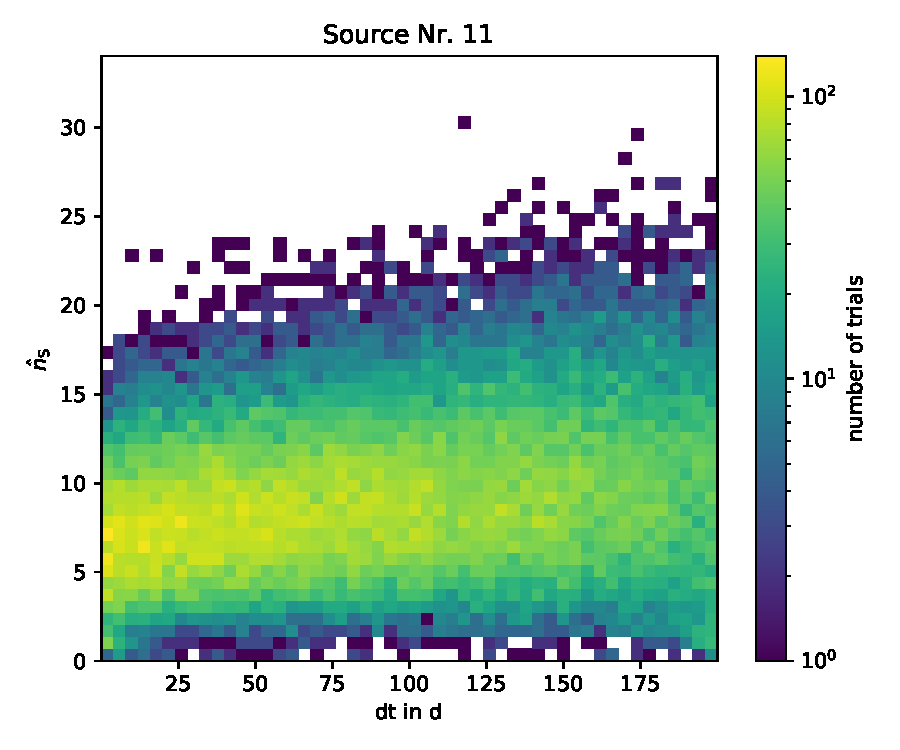
\includegraphics[width=\linewidth]{Plots/05_csky/time_windows_ns_disc_time_dep_1.pdf}
    \caption{Histogram of the time window lengths $dt$ in days in dependence of the fitted signal parameter $\hat{n}_\text{S}$ of source number $\num{11}$ for the time-dependent analysis for the set of signal trials with the number of injected signal events closest to satisfying the condition to calculate the discovery potential.}
    \label{fig:disc_ns_dt}
\end{figure}


\section{Examination of Fit Bias}

\begin{figure}
    \centering
    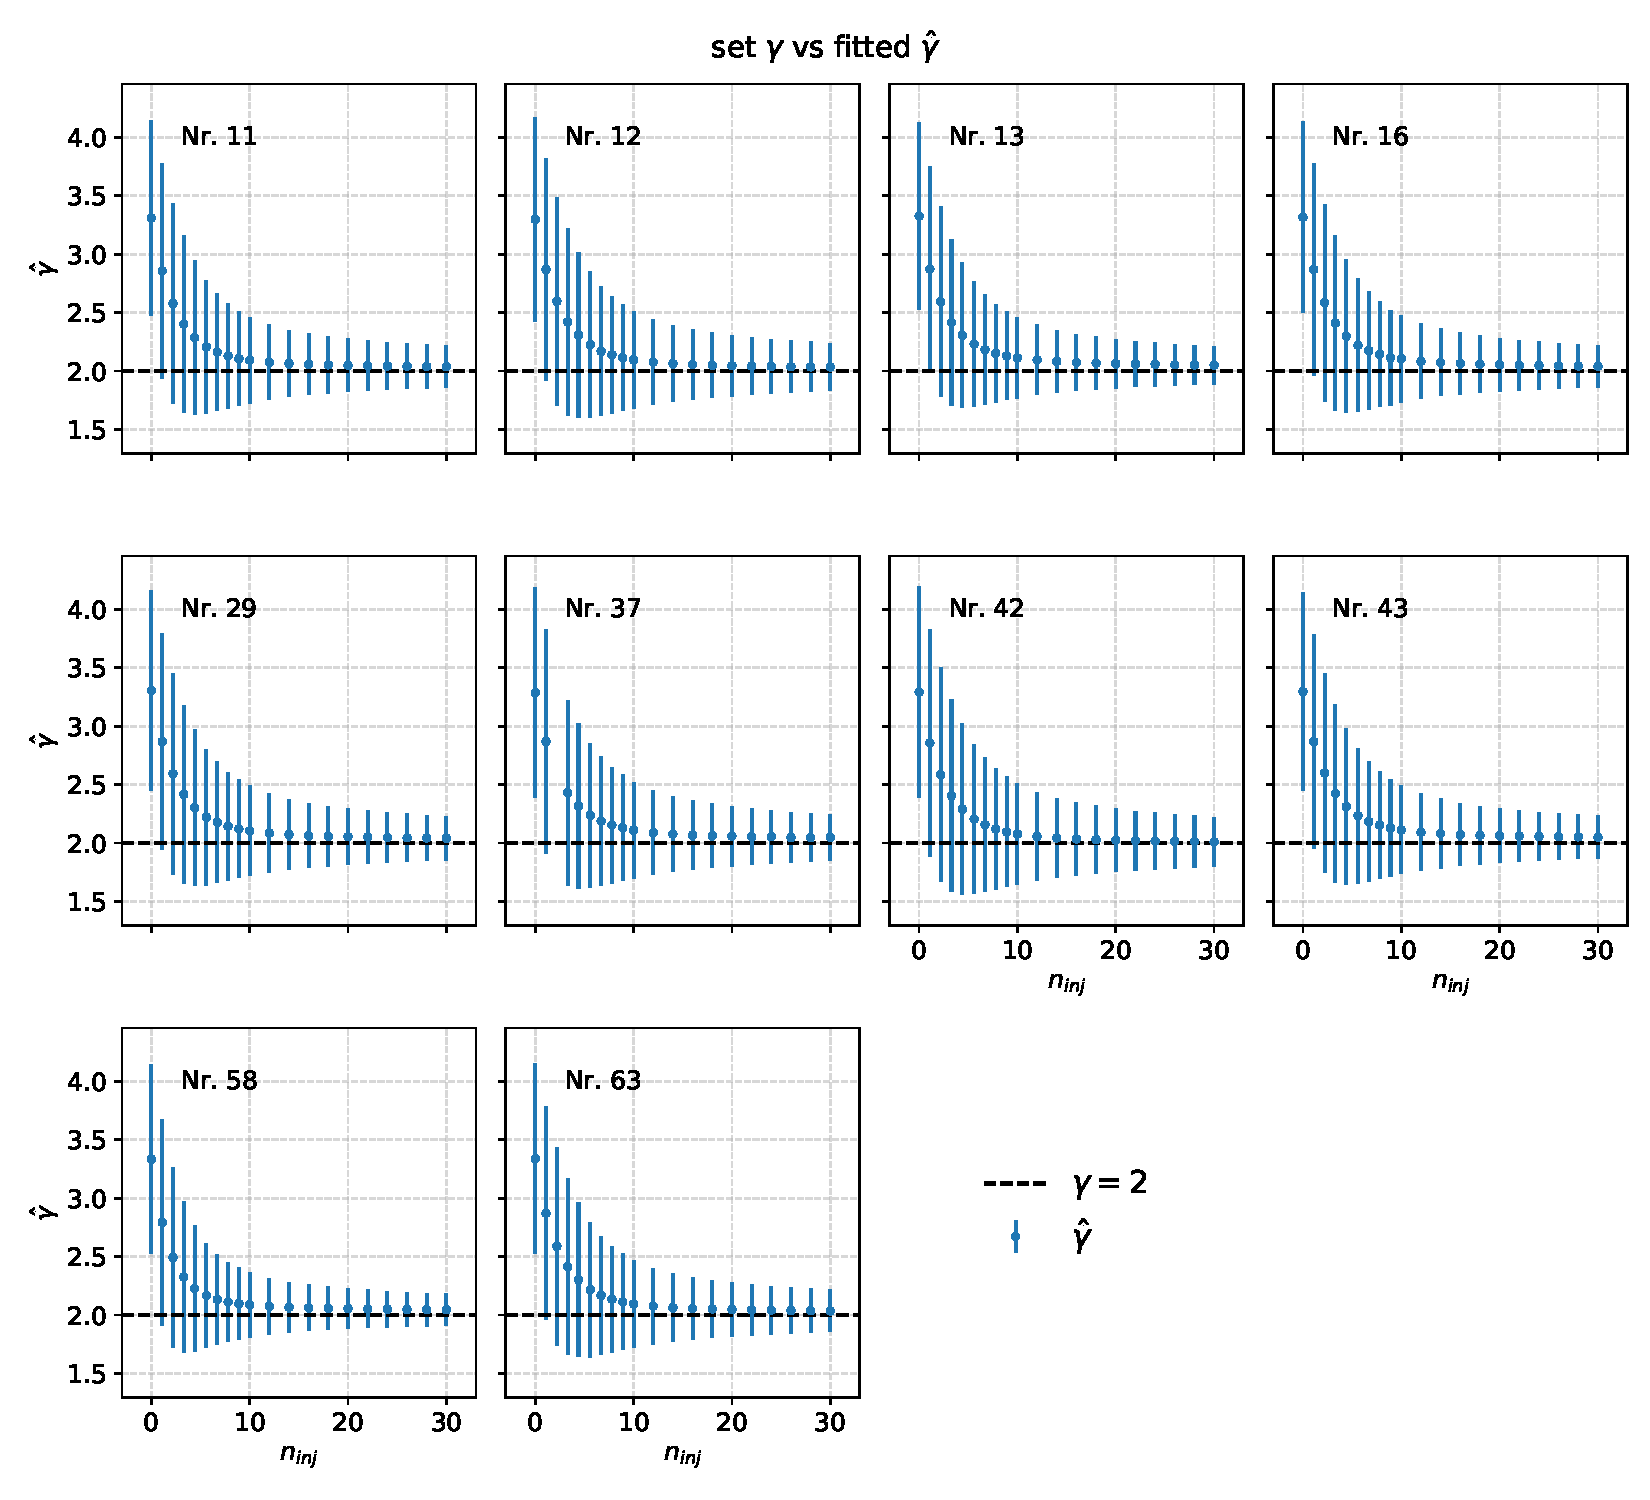
\includegraphics[width=\linewidth]{Plots/05_csky/gamma_fit_time_dep.pdf}
    \caption{Fitted spectral index $\hat\gamma$ in dependence of the injected number of signal events $n_\text{inj}$ with spectral index $\gamma$, shown with a horizontal black dashed line, for the trials used in the time-dependent analysis.}
    \label{fig:gamma_fit_time_dep}
\end{figure}

\begin{figure}
    \centering
    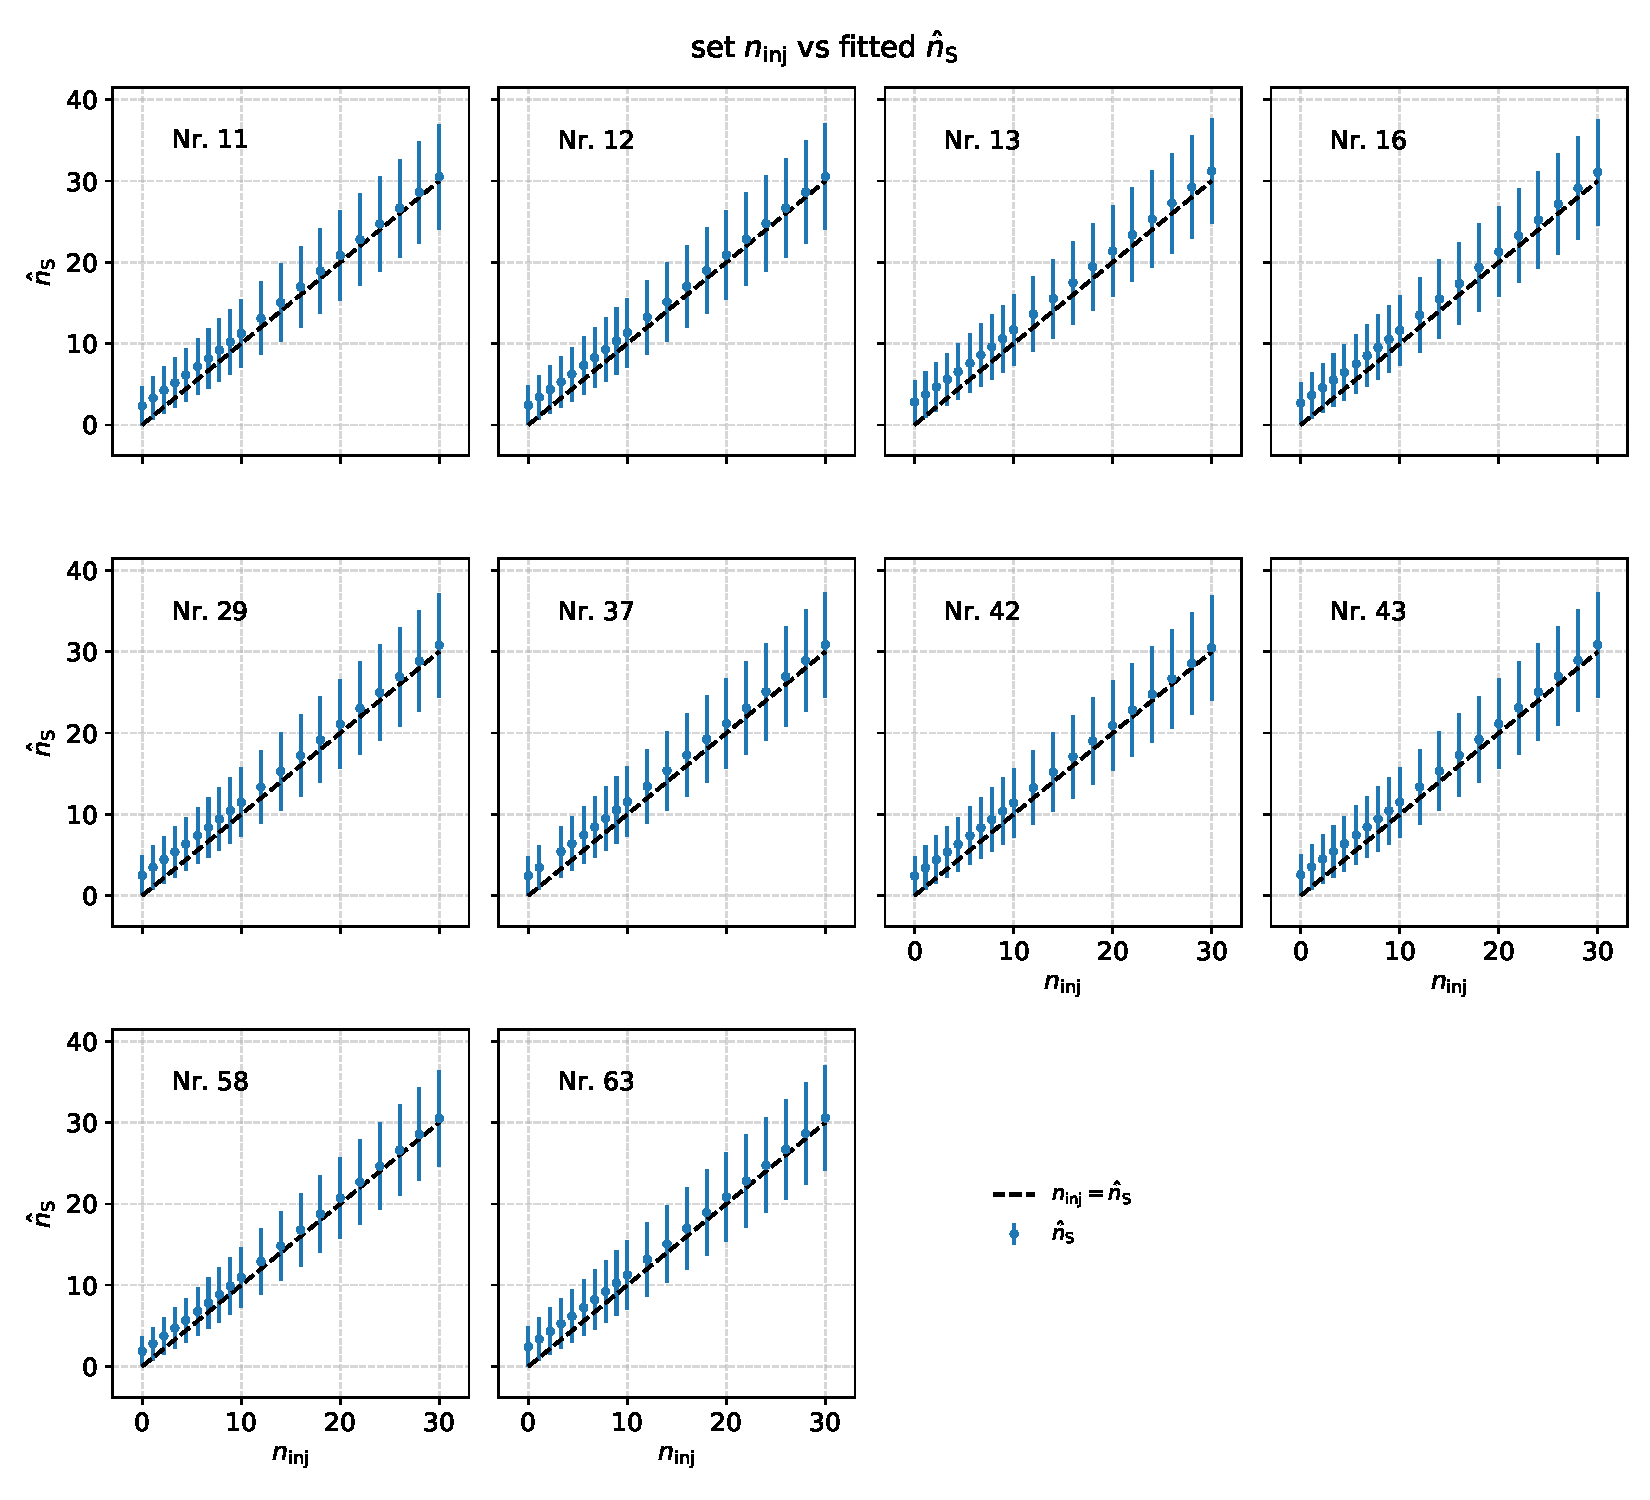
\includegraphics[width=\linewidth]{Plots/05_csky/ns_fit_time_dep.pdf}
    \caption{Fitted number of signal events $\hat{n}_{\text{S}}$ in dependence of the injected number of signal events $n_\text{inj}$ with spectral index $\gamma$ for the time-dependent analysis. The black dashed line shows the equality of fitted and injected number of signal events.}
    \label{fig:ns_fit_time_dep}
\end{figure}

%tdepps stuff
\chapter{Time-Dependent Stacking Software Approach} \label{sec:tdepps}

As already indicated in chapter \ref{sec:csky_time_dep}, a different likelihood must be used to calculate time-dependent stacking.
The test statistic shown in chapter \ref{sec:theory} benefits from the fact that each event is independent of each other and thus PDF ratios can be used directly to calculate the likelihood ratio.
This also benefits the computational capacity.
If, on the other hand, there are several events in the same time window from different sources, these are counted several times and the background is also overestimated.
For a correct calculation, the original test statistic derived in \eqref{eq:TS_general}, which is again shown in equation \eqref{eq:general_ts}, must be considered,
\begin{equation}
    -2\ln{\hat{\Lambda}} = -2\sum_{k=1}^{N_{\text{srcs}}}\hat{\lambda}_{k,S} + 2\sum_{i=1}^{N_{evts}}\ln{\left(\frac{\sum_{k=1}^{N_{\text{srcs}}}\hat{\lambda}_{k,S}S_{i,k}}{\sum_{k=1}^{N_{\text{srcs}}}\langle\lambda_{k,B}\rangle B_{i,k}}+1\right)} \label{eq:general_ts}, \\
\end{equation}
with the expected values for the number of background events $\langle\lambda_{k,B}\rangle$ and signal events  $\hat{\lambda}_{k,S}$ and the PDFs for background $B$ and signal $S$ dependent on the source $k$ and event $i$.
The diagram in figure \ref{fig:new_method} illustrates the problem and the approach to solving it.

\begin{figure}
  \centering
  \scalebox{0.8}{
  \begin{tikzpicture}[scale=1]
    %\node at (2,-6) {\includegraphics[width=10cm]{images/bg_hist_and_contour.pdf}};
    % Koordinatensystem
    \draw[line width=0.25mm, ->] (-5,0) -- (-5,5);
    \draw[line width=0.25mm, ->] (-5,0) -- (10,0);
    \node at (10,-0.5) {time};
    \node at (-5.5,3) {rate};
    % Quellen
    \draw[line width=0.5mm, green] (-1,-1) -- (-1,4);
    \fill[pattern = north east lines, pattern color = green, opacity = 0.5,domain=-3:1,variable=\x]
    (-3,0)
    -- plot ({\x},{3.5})
    -- (1,0)
    -- cycle;
    \fill[pattern = north east lines, pattern color = green, opacity = 0.5,domain=-3:1,variable=\x]
    (-3,0)
    -- plot ({\x},{-0.5})
    -- (1,0)
    -- cycle;
    \draw[green] (-3,-0.5) -- (1,-0.5);
    \draw[green] (-3,3.5) -- (1,3.5);
    \draw[green] (-3,-0.5) -- (-3,3.5);
    \draw[green] (1,-0.5) -- (1,3.5);
    \node[green] at (-1,4.5) {$k=1$};

    \draw[line width=0.5mm, red] (2.5,-1) -- (2.5,4);
    \fill[pattern = north west lines, pattern color = red, opacity = 0.5,domain=0.5:4.5,variable=\x]
    (0.5,0)
    -- plot ({\x},{3.5})
    -- (4.5,0)
    -- cycle;
    \fill[pattern = north west lines, pattern color = red, opacity = 0.5,domain=0.5:4.5,variable=\x]
    (0.5,0)
    -- plot ({\x},{-0.5})
    -- (4.5,0)
    -- cycle;
    \draw[red] (0.5,-0.5) -- (4.5,-0.5);
    \draw[red] (0.5,3.5) -- (4.5,3.5);
    \draw[red] (0.5,-0.5) -- (0.5,3.5);
    \draw[red] (4.5,-0.5) -- (4.5,3.5);
    \node[red] at (2.5,4.5) {$k=2$};

    \draw[line width=0.5mm, blue] (6,-1) -- (6,4);
    \fill[pattern = north east lines, pattern color = blue, opacity = 0.5, domain=4:8,variable=\x]
    (4,0)
    -- plot ({\x},{3.5})
    -- (8,0)
    -- cycle;
    \fill[pattern = north east lines, pattern color = blue, opacity = 0.5,domain=4:8,variable=\x]
    (4,0)
    -- plot ({\x},{-0.5})
    -- (8,0)
    -- cycle;
    \draw[blue] (4,-0.5) -- (8,-0.5);
    \draw[blue] (4,3.5) -- (8,3.5);
    \draw[blue] (4,-0.5) -- (4,3.5);
    \draw[blue] (8,-0.5) -- (8,3.5);
    \node[blue] at (6,4.5) {$k=3$};
    % Samples
    %\draw[line width=0.5mm] (6,-2) -- (6,5);
    %\draw[line width=0.5mm] (0,-2) -- (0,5);
    %\node at (-3,5) {j=1};
    %\node at (3,5) {j=2};
    %\node at (8,5) {j=3};
    % Events
    %\draw[line width=0.5mm,orange] (5,-2) -- (5,1);
    %\draw[line width=0.5mm,orange] (8,-2) -- (8,1);
    %\draw[line width=0.5mm,orange] (3,-2) -- (3,1);
    \draw[line width=0.5mm,orange] (0.75,-1) -- (0.75,1);
    %\node at (0.9,-1.5) {\quad$0.5$};
    %\node at (3.1,-1.5) {\quad$1$};
    %\node at (5.1,-1.5) {\quad$0$};
    %\node at (8.1,-1.5) {\quad$1$};
    \node[orange] at (0.75,-1.5) {$i=1$};
    %\node[orange] at (3,-2.5) {i=2};
    %\node[orange] at (5,-2.5) {i=1};
    %\node[orange] at (8,-2.5) {i=4};
    % Nodes
    %\node at (-1,-1.5) {$T_k(t_i)=$};
    \node[gray] at (-5.8,1.5) {bg-rate};
    % sinus rate
    %\fill [pattern=north east lines,pattern color = blue, domain=2:6, variable=\x]
    %(2, 0)
    %-- plot ({\x}, {sin{(100*\x)}+2})
    %-- (6, 0)
    %-- cycle;
    %\fill [pattern=north east lines,pattern color = red, domain=5:6, variable=\x]
    %(5, 0)
    %-- plot ({\x}, {sin{(100*\x)}+1.5})
    %-- (6, 0)
    %-- cycle;
    %\draw[gray, thick,smooth,domain=0:6 , variable=\x] plot({\x},{0.5*sin{(100*\x)}+2});
    \draw[gray, line width=0.5mm, smooth,domain=-5:0, variable=\x] plot({\x},{0.5*sin{(100*\x)}+1.5});
    \draw[gray, line width=0.5mm, smooth,domain=0:5, variable=\x] plot({\x},{0.5*sin{(100*\x)}+1.5});
    \draw[gray, line width=0.5mm, smooth,domain=5:10, variable=\x] plot({\x},{0.5*sin{(100*\x)}+1.5});
    %\draw[gray, thick,smooth,domain=6:10, variable=\x] plot({\x},{0.5*sin{(100*\x)}+1});
    % intervals
    %\node at (2.5,7.25) {Old method: $\langle\lambda_{B,i=1}\rangle = \langle\lambda_{B,unique}\rangle$};
    %\draw[thick] (-3,7) -- (8,7);
    %\draw[thick] (-3,6.75) -- (-3,7.25);
    %\draw[thick] (8,6.75) -- (8,7.25);
    \node at (0.75,6.25) {New method: $\langle\lambda_{B,i=1}\rangle = \langle\lambda_{B,\{k=1\cup k=2\}}\rangle$};
    \draw[thick] (-3,6) -- (4.5,6);
    \draw[thick] (-3,5.75) -- (-3,6.25);
    \draw[thick] (4.5,5.75) -- (4.5,6.25);
    %thingie
    %\draw[thick, ->] (-5) -- (10);
  \end{tikzpicture}}
  \caption{Scheme illustrating the event attribution of an orange event $i$ and three sources $k$ over time (green, red and blue). The shaded areas of the sources represent their time windows. The grey line symbolises the rate of background events with their seasonal variations. The black interval on top indicates which sources with their time windows must be considered for the event $i$.}
  \label{fig:new_method}
\end{figure}

So for the single event $i$ and two sources the test statistic\footnote{The parameter $w_k$ is the source weight, which is not important for the demonstration in this chapter.} becomes,
\begin{equation}
    -2\ln{\hat{\Lambda}} =-2n_S +2\ln\left(\frac{\frac{n_S}{2}(w_{k=1}\cdot S_{k=1} + w_{k=2} \cdot S_{k=2})}{\langle\lambda_{B,\{k=1\cup k=2\}}\rangle \cdot B_{\{k=1\cup k=2\}}}+1\right) \label{eq:simple_example},
\end{equation}
assuming that $\SI{50}{\percent}$ of the event is attributed evenly to the two sources.
Of course, this ratio could be adjusted to the temporary proximity to the sources, but without further assumptions, the distribution is simply the same.
The basic idea now is that the time interval from which the background is estimated now corresponds to the union of the time windows of the two sources, $B_{\{k=1\cup k=2\}}$ and for the expected number of background events respectively $\langle\lambda_{B,\{k=1\cup k=2\}}\rangle$.
This means that for each possible constellation of time windows and overlaps, a background model must be set up.
The figure \ref{fig:activation} shows qualitatively the activation regions according to which a background model is selected.
\begin{figure}
  \scalebox{0.5}{
  \begin{tikzpicture}[scale=1]
    \node[draw] at (-10,2.5) {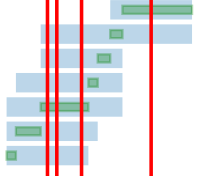
\includegraphics[width=4cm]{Plots/appendix/example.png}};
    % Koordinatensystem
    \draw[line width=0.25mm, ->] (-5,0) -- (-5,5);
    \draw[line width=0.25mm, ->] (-5,0) -- (10,0);
    \node at (10,-0.5) {time};
    \node at (-5.5,3) {rate};
    % Quellen
    \draw[line width=0.5mm, green] (-1,-1) -- (-1,4);
    \fill[pattern = north east lines, pattern color = green, opacity = 0.5,domain=-3:1,variable=\x]
    (-3,0)
    -- plot ({\x},{3.5})
    -- (1,0)
    -- cycle;
    \fill[pattern = north east lines, pattern color = green, opacity = 0.5,domain=-3:1,variable=\x]
    (-3,0)
    -- plot ({\x},{-0.5})
    -- (1,0)
    -- cycle;
    \draw[green] (-3,-0.5) -- (1,-0.5);
    \draw[green] (-3,3.5) -- (1,3.5);
    \draw[green] (-3,-0.5) -- (-3,3.5);
    \draw[green] (1,-0.5) -- (1,3.5);
    \node[green] at (-1,4.5) {$k=1$};

    \draw[line width=0.5mm, orange] (-0.8,-1) -- (-0.8,4);
    \fill[pattern = north east lines, pattern color = orange, opacity = 0.5,domain=-2.8:1.2,variable=\x]
    (-2.8,0)
    -- plot ({\x},{3.5})
    -- (1.2,0)
    -- cycle;
    \fill[pattern = north east lines, pattern color = orange, opacity = 0.5,domain=-2.8:1.2,variable=\x]
    (-2.8,0)
    -- plot ({\x},{-0.5})
    -- (1.2,0)
    -- cycle;
    \draw[orange] (-2.8,-0.5) -- (1.2,-0.5);
    \draw[orange] (-2.8,3.5) -- (1.2,3.5);
    \draw[orange] (-2.8,-0.5) -- (-2.8,3.5);
    \draw[orange] (1.2,-0.5) -- (1.2,3.5);
    \node[orange] at (-0.8,-1.5) {$k=2$};

    \draw[line width=0.5mm, red] (2.5,-1) -- (2.5,4);
    \fill[pattern = north west lines, pattern color = red, opacity = 0.5,domain=0.5:4.5,variable=\x]
    (0.5,0)
    -- plot ({\x},{3.5})
    -- (4.5,0)
    -- cycle;
    \fill[pattern = north west lines, pattern color = red, opacity = 0.5,domain=0.5:4.5,variable=\x]
    (0.5,0)
    -- plot ({\x},{-0.5})
    -- (4.5,0)
    -- cycle;
    \draw[red] (0.5,-0.5) -- (4.5,-0.5);
    \draw[red] (0.5,3.5) -- (4.5,3.5);
    \draw[red] (0.5,-0.5) -- (0.5,3.5);
    \draw[red] (4.5,-0.5) -- (4.5,3.5);
    \node[red] at (2.5,4.5) {$k=3$};

    \draw[line width=0.5mm, blue] (6,-1) -- (6,4);
    \fill[pattern = north east lines, pattern color = blue, opacity = 0.5, domain=4:8,variable=\x]
    (4,0)
    -- plot ({\x},{3.5})
    -- (8,0)
    -- cycle;
    \fill[pattern = north east lines, pattern color = blue, opacity = 0.5,domain=4:8,variable=\x]
    (4,0)
    -- plot ({\x},{-0.5})
    -- (8,0)
    -- cycle;
    \draw[blue] (4,-0.5) -- (8,-0.5);
    \draw[blue] (4,3.5) -- (8,3.5);
    \draw[blue] (4,-0.5) -- (4,3.5);
    \draw[blue] (8,-0.5) -- (8,3.5);
    \node[blue] at (6,4.5) {$k=4$};
    % Samples
    %\draw[line width=0.5mm] (6,-2) -- (6,5);
    %\draw[line width=0.5mm] (0,-2) -- (0,5);
    %\node at (-3,5) {j=1};
    %\node at (3,5) {j=2};
    %\node at (8,5) {j=3};
    % Events
    %\draw[line width=0.5mm,orange] (5,-2) -- (5,1);
    %\draw[line width=0.5mm,orange] (8,-2) -- (8,1);
    %\draw[line width=0.5mm,orange] (3,-2) -- (3,1);
    %\draw[line width=0.5mm,orange] (0.75,-1) -- (0.75,1);
    %\node at (0.9,-1.5) {\quad$0.5$};
    %\node at (3.1,-1.5) {\quad$1$};
    %\node at (5.1,-1.5) {\quad$0$};
    %\node at (8.1,-1.5) {\quad$1$};
    %\node[orange] at (0.75,-1.5) {$i=1$};
    %\node[orange] at (3,-2.5) {i=2};
    %\node[orange] at (5,-2.5) {i=1};
    %\node[orange] at (8,-2.5) {i=4};
    % Nodes
    %\node at (-1,-1.5) {$T_k(t_i)=$};
    %\node[gray] at (-5.8,1.5) {bg-rate};
    % sinus rate
    %\fill [pattern=north east lines,pattern color = blue, domain=2:6, variable=\x]
    %(2, 0)
    %-- plot ({\x}, {sin{(100*\x)}+2})
    %-- (6, 0)
    %-- cycle;
    %\fill [pattern=north east lines,pattern color = red, domain=5:6, variable=\x]
    %(5, 0)
    %-- plot ({\x}, {sin{(100*\x)}+1.5})
    %-- (6, 0)
    %-- cycle;
    %\draw[gray, thick,smooth,domain=0:6 , variable=\x] plot({\x},{0.5*sin{(100*\x)}+2});
    \draw[gray, line width=0.5mm, smooth,domain=-5:0, variable=\x] plot({\x},{0.5*sin{(100*\x)}+1.5});
    \draw[gray, line width=0.5mm, smooth,domain=0:5, variable=\x] plot({\x},{0.5*sin{(100*\x)}+1.5});
    \draw[gray, line width=0.5mm, smooth,domain=5:10, variable=\x] plot({\x},{0.5*sin{(100*\x)}+1.5});
    %\draw[gray, thick,smooth,domain=6:10, variable=\x] plot({\x},{0.5*sin{(100*\x)}+1});
    % intervals
    %\node at (2.5,7.25) {Old method: $\langle\lambda_{B,i=1}\rangle = \langle\lambda_{B,unique}\rangle$};
    %\draw[thick] (-3,7) -- (8,7);
    %\draw[thick] (-3,6.75) -- (-3,7.25);
    %\draw[thick] (8,6.75) -- (8,7.25);
    %\node at (0.75,6.25) {New method: $\langle\lambda_{B,i=1}\rangle = \langle\lambda_{B,\{k=1\cup k=2\}}\rangle$};
    %\draw[thick] (-3,6) -- (4.5,6);
    %\draw[thick] (-3,5.75) -- (-3,6.25);
    %\draw[thick] (4.5,5.75) -- (4.5,6.25);
    %thingie
    %\draw[thick, ->] (-5) -- (10);
    % arrow to picture
    \draw[very thick, ->, color=black] (-5.5,2.5) -- (-7,2.5);
  \end{tikzpicture}}
  \caption{This figure shows a scenario of $\num{4}$ sources $k$ with their time windows (dashed areas). Each unique temporal position translates into a green area on the left, so does a source with a red line. Each green interval is the activation region indicating that an event falling into that region gets compared to an estimated background created in the underlying light blue temporal interval. The scenario therefore generates $\num{7}$ different models. The grey line shows the background rate with its seasonal variations.}
  \label{fig:activation}
\end{figure}
The number of models $\mathcal{B}$ to be calculated in advance can be estimated as,
\begin{equation}
  N_{\text{srcs}} \leq \mathcal{B}\leq 2N_{\text{srcs}}-1, \label{eq:number_of_models}
\end{equation}
with the number of sources $N_{\text{srcs}}$.
So in the worst case scenario this calculation may become about two times slower.
Fortunately, this only affects the spatial PDF and not the energy distribution, as the spatial background depends on the position of the time window due to seasonal variations.
The energy distribution can be extracted from the summation of events and calculated as before.
The temporal PDF is effectively a Heaviside function that attributes the events to the sources weighted by the number of sources they can be attributed to.
With these thoughts in mind, a new injection model needs to be built that injects the right number of background events depending on the temporal position.

To achieve all of the above, the point source software \texttt{tdepps} \cite{tdepps_1} was modified.
The modified version can be found at \cite{tdepps_2}.

However, after the implementation was completed, test results showed unexpected behaviour compared to other software.
The biggest issue are the large values of the test statistics.
A simple example is shown in figure \ref{fig:fail_example}.
Since the correctness of the shape of the test statistic is difficult to assess in the case of a specific time window, in the example the time window is extended over a single complete data set with only one source being investigated.
The behaviour should therefore correspond to a time-integrated search, a $\chi^2$-distribution with only one degree of freedom would be expected, in other words a flat, straight distribution.
However, the modified software still produces too high, signal-like test statistic values, comparable to these of figure \ref{fig:time_dep_sig_sens_ts} in the appendix.
In addition, the behaviour of the \texttt{skylab} software was considered, which is similar to the original behaviour of the unmodified \texttt{tdepps} software.
The \texttt{skylab} result can be seen in figure \ref{fig:skylab}.
\begin{figure}%
    \centering
    \subfloat[\centering Background trials using the reworked \texttt{tdepps} software.]{{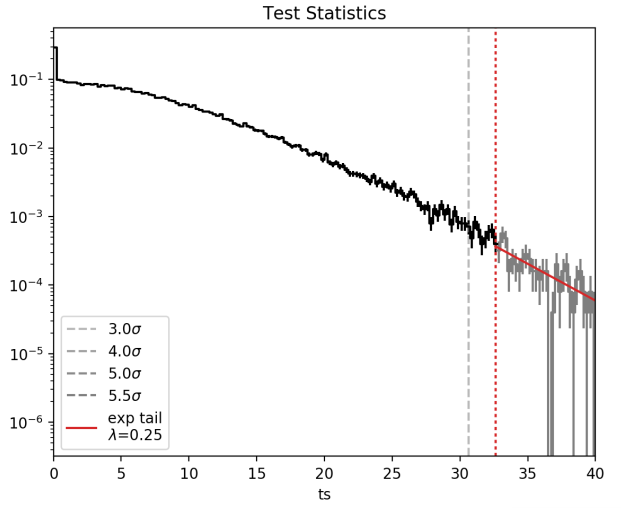
\includegraphics[width=6cm]{Plots/06_tdepps/tdepps_version3_single_bg_pdfs_close.png} }}%
    \qquad
    \subfloat[\centering Background trials using the \texttt{tdepps} software.]{{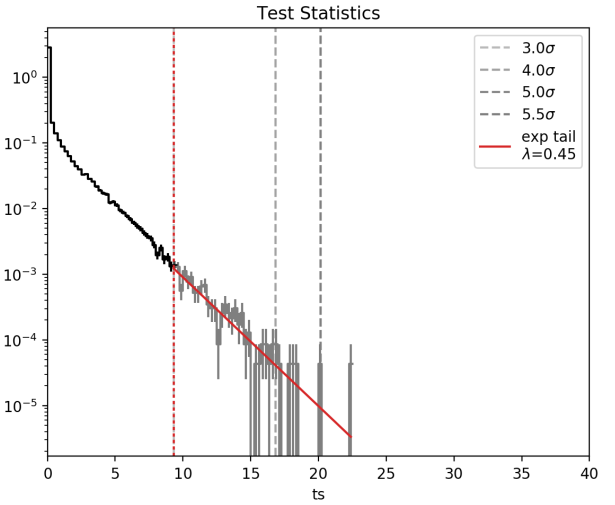
\includegraphics[width=6cm]{Plots/06_tdepps/torben_bg_pdfs_close_real.png} }}%
    \caption{Background trials for $\num{1}$ source with a timewindow expanding over the whole used data set. The y-axis shows the density of trials.}%
    \label{fig:fail_example}%
\end{figure}
\begin{figure}
    \centering
    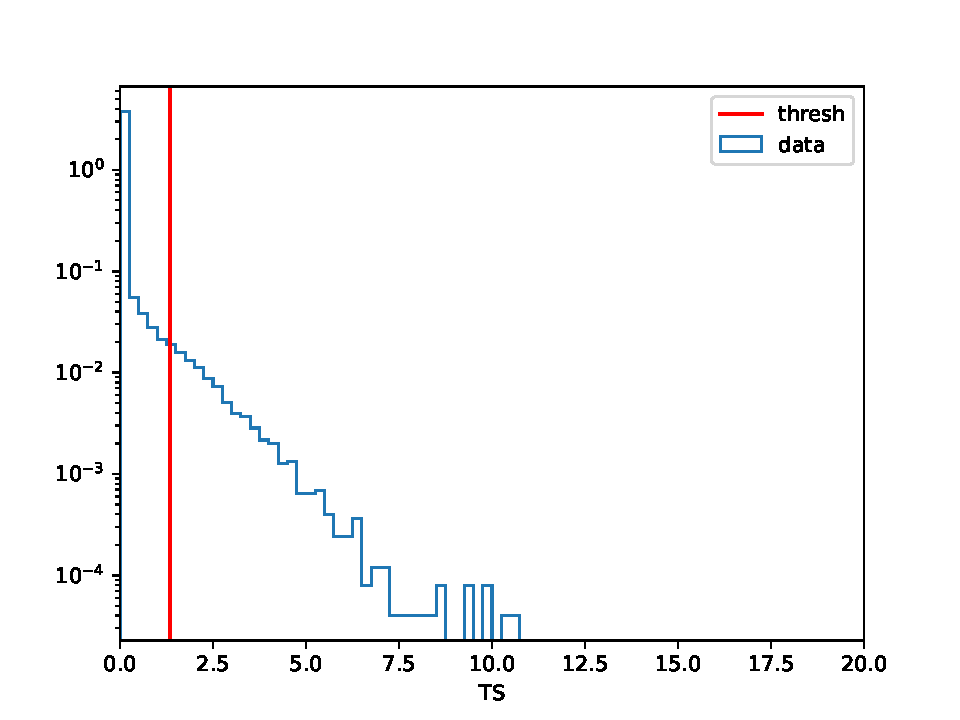
\includegraphics[width=10cm]{Plots/06_tdepps/skylab_bg_pdf_one_source.pdf}
    \caption{Background trials for $\num{1}$ source with a timewindow expanding over the whole used data set using the software \texttt{skylab} version $\num{2.2}$. The y-axis shows the density of trials. The vertical red line indicates the beginning of the straightest possible tail of the statistic determined by various statistical criteria.}
    \label{fig:skylab}
\end{figure}

The main focus of the subsequent research was on the weights that distribute the contribution of the events among the individual sources.
However, this feature works as intended.
Suspicions that this unexpected behaviour could be due to mistakes in the original \texttt{tdepps} software could not be confirmed.
However, as no solution was found to alleviate these problems, the usage of modified \texttt{tdepps} was abandoned.

%both results
\chapter{Conclusion and Outlook} \label{sec:outlook}
are the results measurable?\\
compare both analyses\\
compare with other analyses\\

what could have been done better, whats weird:\\
- mc gfu gold events about times 2: 21002 21220 are weird\\
- source 37 has few trials\\
- more trials; timewindow distribution could be smoother\\
- maybe theres a background event which is an outlier that gets badly scrambled\\
- post trials should be done or all sources\\
- different gammas\\
- take gamma of gfu gold events\\
- spatial errors of sources could be accounted for\\
- take newest version of ps\_tracks\\
why no unblinding?\\
- takes too long\\

All in all, this work provides a good basis for getting started with point source searches using \textbf{csky} and can be used for further analyses by making minor changes.
For example, the data set can be enlarged or additional or different source locations can be investigated.

%outlook moved to previous chapter
%\chapter{Outlook}

%\chapter{Struktur der Arbeit}

Eine mögliche Struktur der Arbeit sieht wie folgt aus:

\begin{enumerate}
    \item \textbf{Einleitung}\\
        In der \emph{kurzen} Einleitung wird die Motivation für die Arbeit
        dargestellt und ein Einblick in die kommenden Kapitel gegeben.
    \item \textbf{Theoretische Grundlagen}\\
        Alles was an theoretischen Grundlagen benötigt wird, sollte auch eher kurz gehalten werden.
        Statt Grundlagenwissen zu präsentieren, eher auf die entsprechenden Lehrbücher verweisen.
        Etwa: Tiefer gehende Informationen zur klassischen Mechanik entnehmen Sie bitte \cite{kuypers}.
    \item \textbf{Ergebnisse} \\
        Der eigentliche Teil der Arbeit, das was getan wurde.
    \item \textbf{Zusammenfassung und Ausblick} \\
        Zusammenfassung der Ergebnisse, Optimierungsmöglichkeiten, mögliche weitergehende Untersuchungen.
\end{enumerate}

Die Gliederung sollte auf der einen Seite nicht zu fein sein, auf der anderen Seite
sollten sich klar unterscheidende Abschnitte auch kenntlich gemacht werden.

In der hier verwendeten \KOMAScript-Klasse \texttt{scrbook} ist die oberste Gliederungsebene,
die in der Bachelorarbeit verwendet werden sollte, das \texttt{\textbackslash chapter}.

Ein Kapitel sollte erst dann in tiefere Gliederungsebenen unterteilt werden, wenn es auch wirklich etwas zu unterteilen gibt. Es sollte keine Kapitel mit nur einem Unterkapitel (\texttt{\textbackslash section}) geben.

In dieser Vorlage ist die Tiefe des Inhaltsverzeichnisses auf \texttt{chapter} und \texttt{section} beschränkt. Möchten Sie diese Beschränkung aufheben, entfernen Sie den Befehl
\begin{verbatim}
            \setcounter{tocdepth}{1}
\end{verbatim}
aus der Präambel oder ändern Sie den Zahlenwert entsprechend. Das Inhaltsverzeichnis sollte für eine Bachelorarbeit auf eine Seite passen.

%\chapter{Wichtige Hinweise zum Dokument}\label{make}

Diese Vorlage ist auf die Kompilierung mit \texttt{lualatex} ausgelegt. 
Als Dokumentenklasse  wird die \KOMAScript\-Klasse \texttt{scrbook} verwendet.
Falls Sie Änderungen am Layout vornehmen möchten, lesen Sie die \KOMAScript-Dokumentation: \cite{koma}.

Eine umfangreiche Einführung in die moderne Verwendung von \LaTeX{} gibt es hier: \cite{toolbox}, lesenswert ist außerdem das \LaTeX-Tabu: \cite{l2tabu}

Um dieses Dokument vollständig zu erstellen sind maximal vier Programmläufe nötig:
\begin{enumerate}[nosep]
    \item \texttt{lualatex BachelorArbeit.tex}
    \item \texttt{biber BachelorArbeit.bcf}
    \item \texttt{lualatex BachelorArbeit.tex}
    \item \texttt{lualatex BachelorArbeit.tex}
\end{enumerate}

Beim ersten Lauf des \LaTeX-Compilers werden die Kapitel, Links und zitierten Bibliographieeinträge in Hilfsdateien geschrieben.

Dann ist ein Lauf des Programms \texttt{biber} nötig, welches die benötigten Einträge aus der Hilfsdatei einliest, die Einträge aus der \texttt{.bib} Datei einliest, sortiert und formatiert und in eine weitere Hilfsdatei schreibt.

Beim nächsten \LaTeX-Lauf werden dann diese Hilfsdateien eingelesen und Literatur- und Inhaltsverzeichnis erstellt.

Manchmal ist ein vierter Lauf nötig, falls sich durch das einfügen des Literaturverzeichnisses Seitenzahlen verändert haben.

Das Tool \texttt{latexmk} übernimmt dies mit nur einem Programmaufruf und
führ nur so viele Aufrufe durch, wie nötig sind.

\texttt{latexmk --lualatex BachelorArbeit.tex}

Eine gute Option ist es, den \LaTeX{} Output in einem anderen 
Ordner zu erzeugen, dies ist mit der \texttt{--output-directory} Option möglich:

\texttt{latexmk --output-directory=build --lualatex BachelorArbeit.tex}


\section{Erstellen des Ausgabedokuments mit Make}

Für diese Vorlage wird ein Makefile zur Verfügung gestellt, welches automatisch alle Schritte ausführt, die für das fertige Dokument nötig sind.
Die Ausgabe erfolgt dabei in den Unterordner \texttt{build/}.
Make prüft, ob die Quelldateien verändert wurden, falls nicht, werden auch keine Befehle ausgeführt.

Falls Sie das Makefile benutzen möchten, sollten Sie alle Abhängigkeiten eintragen (Eigene Dateien für Kapitel, Plots, etc.).


Download und weitere Informationen zu Make gibt es unter \cite{make}. Die Befehle sind für die Bash ausgelegt.
Wenn Sie sie unter Windows nutzen wollen, benötigen Sie einen Bash-Emulator, wie Git Bash, Download unter \cite{gitbash} möglich.
Wenn Sie Make installiert haben, rufen Sie einfach in der Konsole im Verzeichnis der Arbeit den Befehl \texttt{make}.

\section{Erstellen des Ausgabedokuments mit Texmaker}
\subsection{Einrichten der nötigen Befehle}
Ein beliebter Editor für alle Betriebssysteme ist Texmaker, Download unter \cite{texmaker}.
Damit Texmaker das Dokument korrekt kompiliert, fügen sie einen benutzerdefinierten Befehl hinzu:
\begin{enumerate}[nosep]
    \item Klicken sie oben in der Menüleiste auf \emph{Benutzer/in}
    \item Klick auf \emph{Eigene Befehle}
    \item Klich auf \emph{Eigene Befehle editieren}, dort können Sie bis zu 5 eigene Befehle definieren
    \item Geben Sie dem Befehl unter \emph{Menüeintrag} einen Namen und tragen sie folgende Befehle in das Befehlsfeld ein: \\
      \small\verb+latexmk --lualatex --interaction=batchmode --halt-on-error %.tex |+
    \item Bestätigen Sie mit \emph{OK}
\end{enumerate}

\begin{figure}
    \centering
    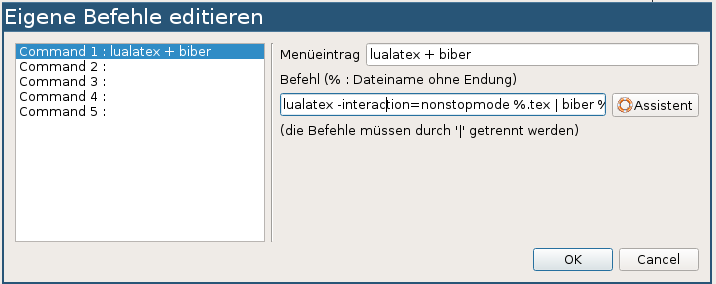
\includegraphics[width=12cm]{Plots/texmaker.png}
    \caption{Screenshot zur Erstellung des Kompilier-Befehls in Texmaker}
    \label{fig:texmaker}
\end{figure}


In Abbildung \ref{fig:texmaker} ist ein Screenshot des Befehlsmenü gezeigt. Ihren Befehl können Sie nun im Drop-Down-Menü zum 
Kompilieren des Dokuments auswählen und mit einem Klick auf den Pfeil starten.

\subsection{Aufräumen}

Nach einem \LaTeX-Fehler ist es oft notwendig, die erstellten Hilfsdateien zu löschen.
Klicken Sie hierzu auf \emph{Werkzeuge}→\emph{Aufräumen}.


\chapter{\LaTeX-Grundlagen}

Bitte beachten Sie beim Schreiben der Arbeit folgende Konventionen bzw. Grundlagen:

\begin{itemize}
    \item \textbf{Abschnitte und Zeilenumbrüche} \\
        Es sollten im Fließtext keine Zeilenumbrüche mit \textbackslash\textbackslash \ erzwungen werden.
        Schreiben Sie höchsten einen Satz in eine Code-Zeile.
        Absätze werden im Code mit einer Leerzeile markiert und dann entsprechend der Einstellung von \texttt{parskip} in der Dokumentenklasse gesetzt.
    \item \textbf{Kursiv/Aufrecht} \\
        \begin{itemize}
            \item Variablen und physikalische Größen werden kursiv gesetzt. 
            \item Einheiten werden immer aufrecht und mit einem halben Leerzeichen Abstand zur Zahl gesetzt. Nutzen Sie \texttt{siunitx}!
            \item Mathematische Konstanten und Funktionen werden ebenfalls aufrecht gesetzt. Zum Beispiel die Eulersche Zahl e, das imaginäre i und das infinitesimale d.
                Im Mathematikmodus können Sie dies mit dem Befehl \verb_\mathrm{}_ erreichen. Für die Funktionen stellt \LaTeX \ Befehle bereit, z.B. \verb+\arccos+.
            \item Integrand und ein $\mathrm{d}x$ sollten ebenfalls durch ein kleines Leerzeichen (\verb+\,+) getrennt werden.
        \end{itemize}
        


\end{itemize}

\section{Zahlen und Einheiten}

Jede Zahl, jede Einheit und jede Zahl mit Einheit sollte mit Hilfe der in dem Paket \texttt{siunitx} zur Verfügung gestellten Befehle gesetzt werden.
Grundsätzlich gilt: Einheiten werden aufrecht gesetzt und haben ein kleines Leerzeichen (\verb+\,+) Abstand zu ihrer Zahl. 
Werden Fließkommazahlen ohne \texttt{siunitx} gesetzt, entsteht ein hässlicher Leerraum zwischen Komma und erster Nachkommastelle, da \LaTeX \ das Komma nicht als Dezimaltrennzeichen, sondern als Satzzeichen interpretiert.

Das Paket wurde mit deutschen Spracheinstellungen (also mit Komma als Dezimaltrennzeichen und $\cdot$ zwischen Zahl und Zehnerpotenz) geladen, sowie mit den Einstellungen, dass die Standardabweichung stets durch $\pm$ abgetrennt wird und Einheiten falls nötig als Brüche ausgegeben werden.

\begin{table}
    \centering
    \caption{Beispiele für siunitx}
    \label{tab:si}
    \begin{tabular}{l r}
        \toprule
        Befehl     &   Ergebnis \\
        \midrule
        \verb+\num{1.2345}+ & \num{1.2345} \\
        \verb+\num{1.2e3}+ & \num{1.2e3} \\
        \verb_\num{1.2 +- 0.2}_ & \num{1.2+-0.2} \\
        \verb+\num{10000}+ & \num{10000} \\
        \verb+\si{\meter\per\second}+ & \si{\meter\per\second} \\
        \verb+\SI{1.2(1)}{\micro\ampere}+ & \SI{1.2(1)}{\micro\ampere} \\
        \verb+\SI{1.2\pm0.1e3}{\kilo\gram\per\cubic\meter}+ & \SI{1.2\pm0.1e3}{\kilo\gram\per\cubic\meter} \\
        \bottomrule 
    \end{tabular}
\end{table}

Das Paket stellt unter anderem die drei wichtigen Befehle
\begin{itemize}
    \item \texttt{\textbackslash num\{Zahl\}},
    \item \texttt{\textbackslash si\{Einheit\}} und
    \item \texttt{\textbackslash SI\{Zahl\}\{Einheit\}}
\end{itemize}
zur Verfügung.
Diese Befehle sollten stets genutzt werden, wenn Zahlen angegeben werden. 
Sie funktionieren sowohl im Text- als auch im Mathematikmodus.
In Tabelle \ref{tab:si} sind einige Beispiele aufgetragen. Bitte lesen Sie die Dokumentation \cite{siunitx}.

\section{Das Literaturverzeichnis}

Das Literaturverzeichnis wird mit Hilfe von BibLaTeX und biber erstellt.
Tragen Sie alle ihre Quellen in die Datei \texttt{references.bib} ein, Sie enthält bereits
einige Beispiele. Für weitere Informationen lesen Sie bitte die Dokumentation \cite{biblatex}.

Im Text können Sie mit \verb_\cite{kürzel}_ zitieren. Seitenzahlen geben Sie in eckigen Klammern an:
\verb_\cite[10]{kürzel}_. 

Das Literaturverzeichnis ist so eingestellt, dass es Ihre Quellen in alphabetischer Reihenfolge nach Autoren nummeriert.
Möchten Sie das Literaturverzeichnis nach der Reihenfolge des Auftauchens im Text sortieren, fügen sie die Paktetoption \texttt{sorting=none} beim Laden
des BibLaTeX-Pakets hinzu.

Den Zitier- und Bibliographie-Stil geben sie mit der Option \texttt{style=Stil} an. Die beiden gebräuchlisten Stile sind \texttt{numeric} und \texttt{alphabetic}. 
Bei \texttt{numeric} werden die Quellen durchnummeriert, bei \texttt{alphabetic} wird ein Buchstabenkürzel aus Autor(en)-Name(n) und Jahr verwendet.
Für weitere Stile konsultieren Sie bitte die Dokumentation: \cite{biblatex}.

Ein Beispiel für das Zitieren eines Buches lautet so \cite{handbook_adhesives},
wissenschaftliche Artikel hingegen werden so \cite{einstein} zitiert.

Damit das Literaturverzeichnis erstellt wird, ist ein Aufruf von \texttt{biber} nach einem ersten kompilieren mit \texttt{lualatex} nötig.
Danach muss das Dokument erneut mit \texttt{lualatex} kompiliert werden. 

Zum korrekten Kompilieren des Dokuments siehe Kapitel \ref{make}.

%\chapter{Abbildungen und Tabellen}

\section{Abbildungen}

Achten Sie bei ihren Plots auf ausreichend große Achsenbschriftungen, ausreichende Schriftdicken und gut unterscheidbare Farben.
Im Idealfall haben Sie im Plot und der Arbeit die gleiche Schriftgröße und Schriftart.
Dies lässt sich durch Erstellen des Plots in der korrekten Größe und Einbinden mit dem optionalen Argument \texttt{scale=1} erreichen. Ein Beispiel sehen Sie in Abbildung \ref{fig:bsp}.

Nutzen Sie wenn möglich Vektorgrafiken (pdf) und nur in Ausnahmen Rastergrafiken wie .png oder .jpg.
Setzen Sie Punkte hinter Abbildungsunterschriften.

\begin{figure}
    \centering
    \includegraphics[scale=1]{./Plots/Histogramm.pdf}
    \caption{Ein Histogramm mit Fehlerbalken für zwei Datensätze, Schriftgröße und -art entsprechen der des Dokuments.}
    \label{fig:bsp}
\end{figure}

\section{Tabellen}

Tabellen sollten so einfach wie möglich aufgebaut sein, verzichten Sie auf zu viele Linien. In fast allen Fällen reichen drei horizontale Linien aus, jeweils über und unter der Tabelle und zwischen den Spaltenüberschriften und der eigentlichen Tabelle.

Das Paket \texttt{booktabs} stellt hierfür \verb_\toprule_, \verb_\midrule_ und 
\verb_\bottomrule_ zur Verfügung.
Das Paket \texttt{siunitx} stellt eine extrem mächtige neue Spalteneinstellung bereit: \texttt{S}, mit ihr können Zahlen und Einheiten sehr sauber und gut ausgerichtet gesetzt werden.

Diese Vorlage geht von Tabellenüberschriften aus, möchten Sie dagegen Tabellenunterschriften entfernen Sie das entsprechende optionale Argument für die Dokumentenklasse in der Präambel.

Ein Beispiel ist Tabelle~\ref{tab:bsp}.
\begin{table}
    \centering
    \caption{Beispieltabelle mit willkürlichen Werten, für die Zahlenwerte wurde die S-Option aus \texttt{siunitx} verwendet.}
    \label{tab:bsp}
    \begin{tabular}{S[table-format=4.2] S[table-format=3.2]}
        \toprule
        {$p \mathrel{/} \si{\pascal}$}  & {$T \mathrel{/} \si{\kelvin}$} \\
        \midrule
        1024,23 & 273,15 \\
        1025,31 & 274,5 \\
        1026,27 & 276,2 \\
        \bottomrule
    \end{tabular}
\end{table}


\appendix
% Hier beginnt der Anhang, nummeriert in lateinischen Buchstaben
%appendix
\chapter{Supplementary Material} \label{sec:appendix}

This chapter contains supplementary material for additional insight, as well as plots that provide more qualitative information.
In addition, some tables are included here that provide more detailed insights into the data compilation process.
Everything is arranged chronologically according to occurrence in the main section and shares the headline of each chapter for easy reference.

\section{Astroparticle physics}

\begin{figure}
    \centering
    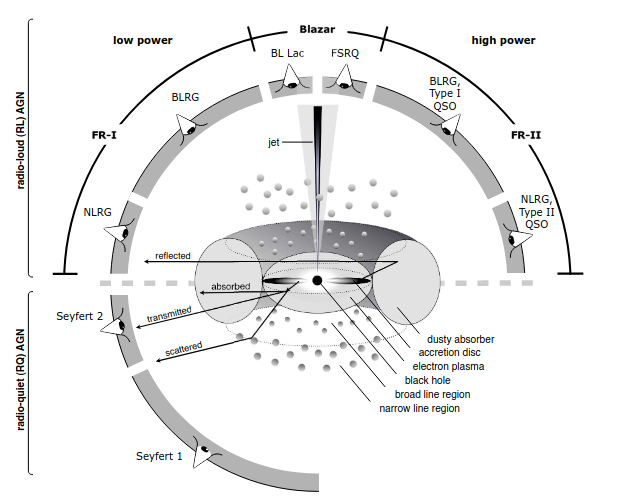
\includegraphics[width=\linewidth]{Plots/appendix/agn.png}
    \caption{This diagram shows the unified AGN scheme \cite{agn}. With blazars, the observer looks more or less directly into the jet of the radioloud AGN.}
    \label{fig:agn}
\end{figure}

\section{Theory}

This scheme is designed to facilitate understanding of sensitivity and discovery potential.

\begin{figure}
  \begin{tikzpicture}[
declare function={gamma(\z)=
2.506628274631*sqrt(1/\z)+ 0.20888568*(1/\z)^(1.5)+ 0.00870357*(1/\z)^(2.5)- (174.2106599*(1/\z)^(3.5))/25920- (715.6423511*(1/\z)^(4.5))/1244160)*exp((-ln(1/\z)-1)*\z;},
declare function={gammapdf(\x,\k,\theta) = 1/(\theta^\k)*1/(gamma(\k))*\x^(\k-1)*exp(-\x/\theta);}]
\begin{axis}[ymode=log, ymin=0,
no markers, domain=0:9, samples=100,
axis lines=left, xlabel=$\text{TS}$, ylabel=$\#\text{trials}$,
y label style={at={(axis description cs:-0.1,.5)},anchor=north},
x label style={dashed,at={(axis description cs:0.95,-0.1)},anchor=west},
height=5cm, width=9cm,
xtick={6,14.87}, ytick=\empty,
xticklabels={$\text{bg median}$,$5\sigma$},
%xticklabels={$\bar n (\theta_t)$},
enlargelimits=false, clip=false,% axis on top,
grid = major]
\addplot [very thick,cyan!20!black,domain=0:20, draw=none] {gammapdf(x,0.2,5)};
\addplot [very thick,cyan!20!black,domain=0.5:19.5] {gammapdf(x,0.2,5)};
%\addplot [domain= 0.5:4.5]{gauss(2.5,0.6,2)};
%\addplot [fill=cyan!20, draw=none, domain=0:6.0] {gammapdf(x,2,2)} \closedcycle;
%\addplot [very thick, fill=white!20!white, draw=none, domain=6.01:20] {gammapdf(x,2,2)} \closedcycle;
\end{axis}
\node at (2.5,1.7) {\begin{tikzpicture} \begin{axis}[hide axis,enlargelimits=false, ymax = 1,height=5cm, width=4cm,domain=2.65:3.35]\addplot [domain= 2.65:3.35,smooth,thick,green]{gauss(3,0.1,0.2)}; \end{axis} \end{tikzpicture}};
\node at (5.5,1.7) {\begin{tikzpicture} \begin{axis}[hide axis,enlargelimits=false, ymax = 1,height=5cm, width=3.5cm,domain=2.7:3.3]\addplot [domain= 2.7:3.3,smooth,thick,red]{gauss(3,0.07,0.14)}; \end{axis} \end{tikzpicture}};
\node[green] at (2.7,3) {$\xrightarrow{\text{90\%}}$};
\node[red] at (6,3) {$\xrightarrow{\text{50\%}}$};
\node at (0.5,3) {$\text{bg}$};
\node[green] at (2.7,4) {$\text{sensitivity}$};
\node[red] at (6,4) {$\text{discovery}$};
\end{tikzpicture}
\caption{Schematic showing the conditions to calculate the sensitivity and discovery potential. The background test statistic is shown in black, the signal test statistic satisfying the sensitivity conditions in green and the one for the discovery potential in red. Note that the curves dont actually look like these shown here. They have been simplified for explanatory purpose.}
\label{fig:sens_disc_schem}
\end{figure}

\section{Sources}

\begin{figure}
    \centering
    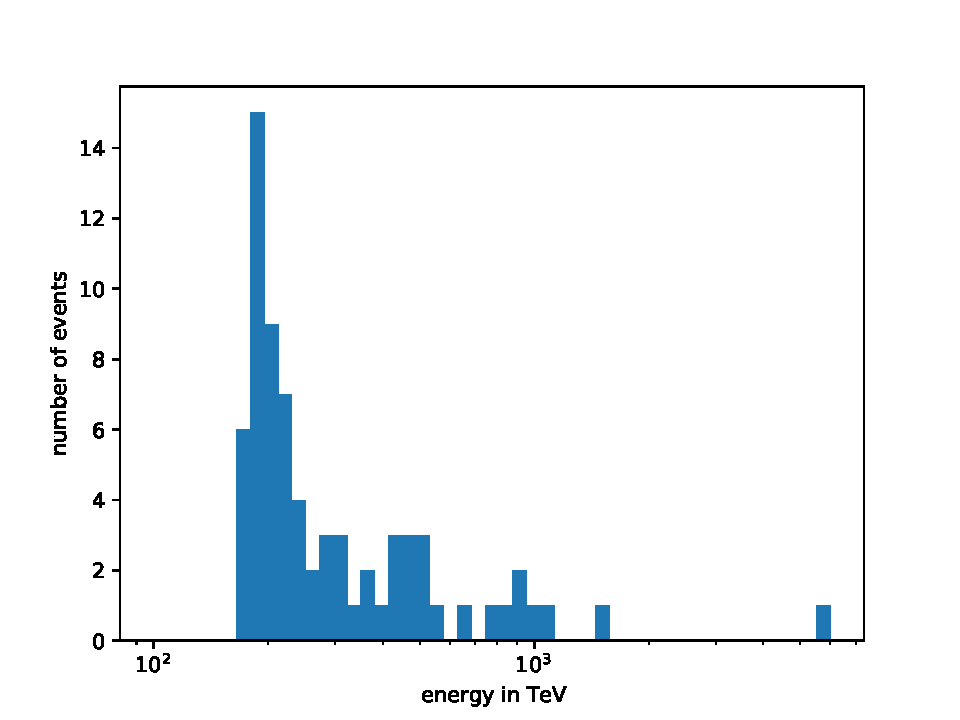
\includegraphics[width=\linewidth]{Plots/appendix/sources_energy.pdf}
    \caption{Histogram of the energy of the used sources seen in table \ref{tab:sources} in $\si{\tera\electronvolt}$.}
    \label{fig:sources_energy}
\end{figure}

\begin{table}
  \centering
  \caption{Table of the sources used in the time-dependent analysis. Additionally the signalness parameter is shown after which the sources were selected.}
  \label{tab:sources_time_dep}
  \begin{tabular}{ccrrc}
    \toprule
    Nr. & MJD &  $\delta$ in $\si{\degree}$ & $\alpha$ in $\si{\degree}$ & signalness in $\si{\percent}$ \\
    \toprule
      11 & 56819.20 & 11.45 & 110.65 & 99.70 \\ 12 & 56470.11 & 14.17 & 93.74 & 93.80 \\ 13 & 57951.82 & 25.16 & 208.39 & 86.60 \\ 16 & 58063.78 & 7.44 & 340.14 & 97.50 \\ 29 & 57340.87 & 12.71 & 76.16 & 95.70 \\ 37 & 55911.28 & 18.88 & 36.74 & 94.60 \\ 42 & 56226.60 & 27.91 & 169.80 & 92.60 \\ 43 & 56666.50 & 33.02 & 293.12 & 92.70 \\ 58 & 57478.57 & 15.48 & 151.22 & 85.10 \\ 63 & 56211.77 & -2.28 & 205.14 & 84.20 \\ 
    \toprule
  \end{tabular}
\end{table}

\section{Time-Integrated Search}

\begin{table}
  \centering
  \caption{Table of the number of injected signal events used for the time integrated analysis.}
  \label{tab:sig_time_int_table}
  \begin{tabular}{r}
    \toprule
    $n_\text{S}$ injected \\
    \toprule
      0.0 \\ 7.5 \\ 15.0 \\ 22.5 \\ 30.0 \\ 36.0 \\ 57.0 \\ 78.0 \\ 99.0 \\ 120.0 \\ 141.0 \\ 194.2 \\ 247.4 \\ 300.7 \\ 353.9 \\ 407.1 \\ 460.3 \\ 513.6 \\ 566.8 \\ 620.0 \\ 
    \toprule
  \end{tabular}
\end{table}

\begin{table}
  \caption{Table of the number of trials for each spectral index $\gamma$ and number of injected signal events $n_\text{sig}$, running $\num{10}$ jobs with $\num{5e3}$ trials per set of parameter pairs $\gamma$ and $n_\text{sig}$. Some jobs fail due to technical reasons.}
  \label{tab:trials_sig_time_int_table}
  \begin{subtable}{\linewidth}
  \centering
  \begin{tabular}{p{.9cm}|rrrrrrrrrr}
    \toprule
    \: $n_\text{sig}$ \newline $\gamma$ \: & 0.0 & 7.5 & 15.0 & 22.5 & 30.0 & 36.0 & 57.0 & 78.0 & 99.0 & 141.0 \\ 
    \toprule
    1.50 & 50000 & 50000 & 50000 & 50000 & 50000 & 50000 & 50000 & 50000 & 50000 & 50000 \\ 1.75 & 50000 & 50000 & 50000 & 50000 & 50000 & 50000 & 50000 & 50000 & 50000 & 50000 \\ 2.00 & 50000 & 50000 & 50000 & 50000 & 50000 & 50000 & 50000 & 50000 & 50000 & 50000 \\ 2.25 & 50000 & 45000 & 45000 & 45000 & 50000 & 45000 & 50000 & 50000 & 50000 & 50000 \\ 2.50 & 50000 & 50000 & 50000 & 50000 & 50000 & 50000 & 50000 & 50000 & 50000 & 50000 \\ 2.75 & 50000 & 50000 & 45000 & 45000 & 50000 & 50000 & 50000 & 40000 & 50000 & 40000 \\ 3.00 & 50000 & 50000 & 50000 & 50000 & 50000 & 45000 & 50000 & 50000 & 50000 & 50000 \\ 
    \toprule
  \end{tabular}
\end{subtable}
\begin{subtable}{\linewidth}
\centering
  \begin{tabular}{p{.9cm}|rrrrrrrrrr}
    \toprule
    \: $n_\text{sig}$ \newline $\gamma$ \: & 141.0 & 194.2 & 247.4 & 300.7 & 353.9 & 407.1 & 460.3 & 513.6 & 566.8 & 620.0 \\ 
    \toprule
    1.50 & 50000 & 50000 & 50000 & 50000 & 50000 & 50000 & 50000 & 50000 & 50000 & 50000 \\ 1.75 & 50000 & 50000 & 50000 & 50000 & 50000 & 50000 & 50000 & 50000 & 50000 & 45000 \\ 2.00 & 50000 & 50000 & 50000 & 50000 & 50000 & 50000 & 50000 & 50000 & 50000 & 50000 \\ 2.25 & 50000 & 50000 & 50000 & 50000 & 50000 & 50000 & 50000 & 50000 & 50000 & 50000 \\ 2.50 & 50000 & 50000 & 50000 & 50000 & 50000 & 50000 & 50000 & 50000 & 50000 & 40000 \\ 2.75 & 50000 & 50000 & 50000 & 50000 & 50000 & 50000 & 50000 & 50000 & 50000 & 50000 \\ 3.00 & 50000 & 50000 & 45000 & 50000 & 50000 & 50000 & 50000 & 50000 & 50000 & 50000 \\ 
    \toprule
  \end{tabular}
  \end{subtable}
\end{table}

\section{Time-Dependent Search} \label{sec:time_dep_search_appendix}

In this chapter the complete results for all $\num{10}$ sources can be found.

\subsection{Background Trials}

\begin{figure}
    \centering
    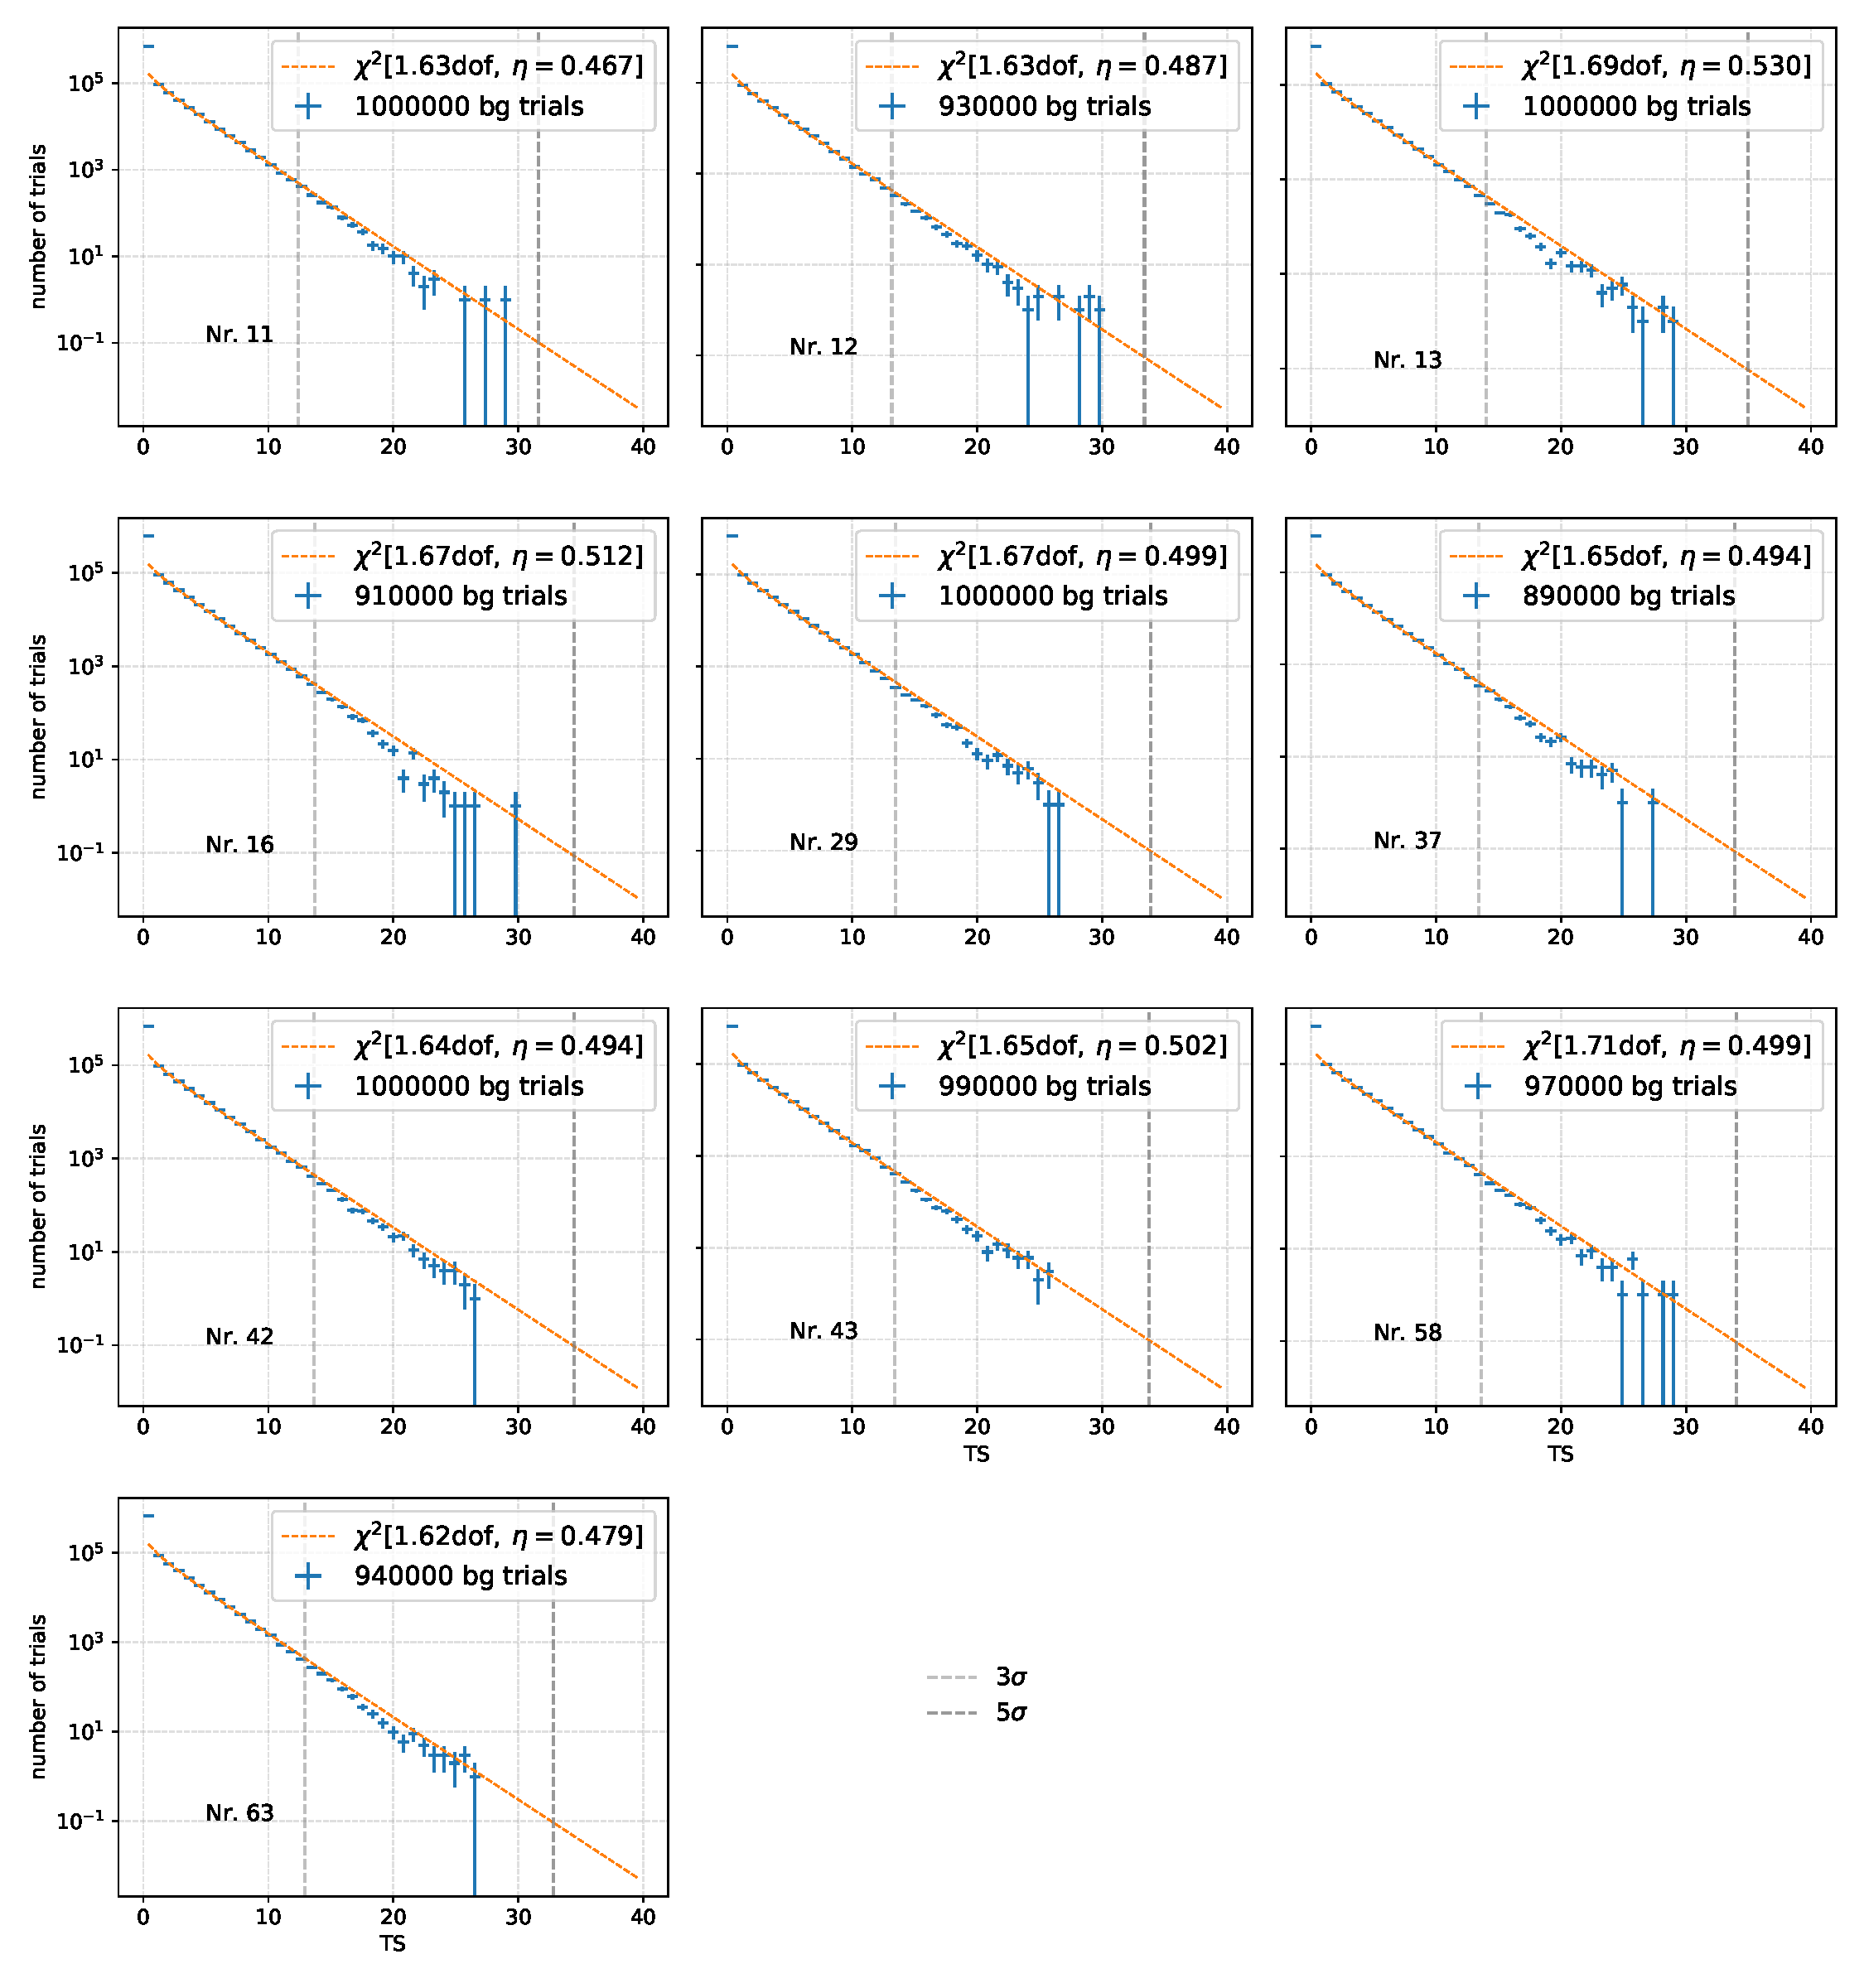
\includegraphics[width=\linewidth-2cm]{Plots/05_csky/9_years_gfu_gold_time_dep_bg_t0.pdf}
    \caption{Histograms of the background test statistic values for all $\num{10}$ sources used in the time-dependent analysis. Shown are also the number of degrees of freedom $dof$ and the ratio of positive and negative values $\eta$. The id of the sources corresponds to table \ref{tab:sources} or \ref{tab:sources_time_dep} respectively.}
    \label{fig:bg_trials_time_dep}
\end{figure}

\begin{figure}
    \centering
    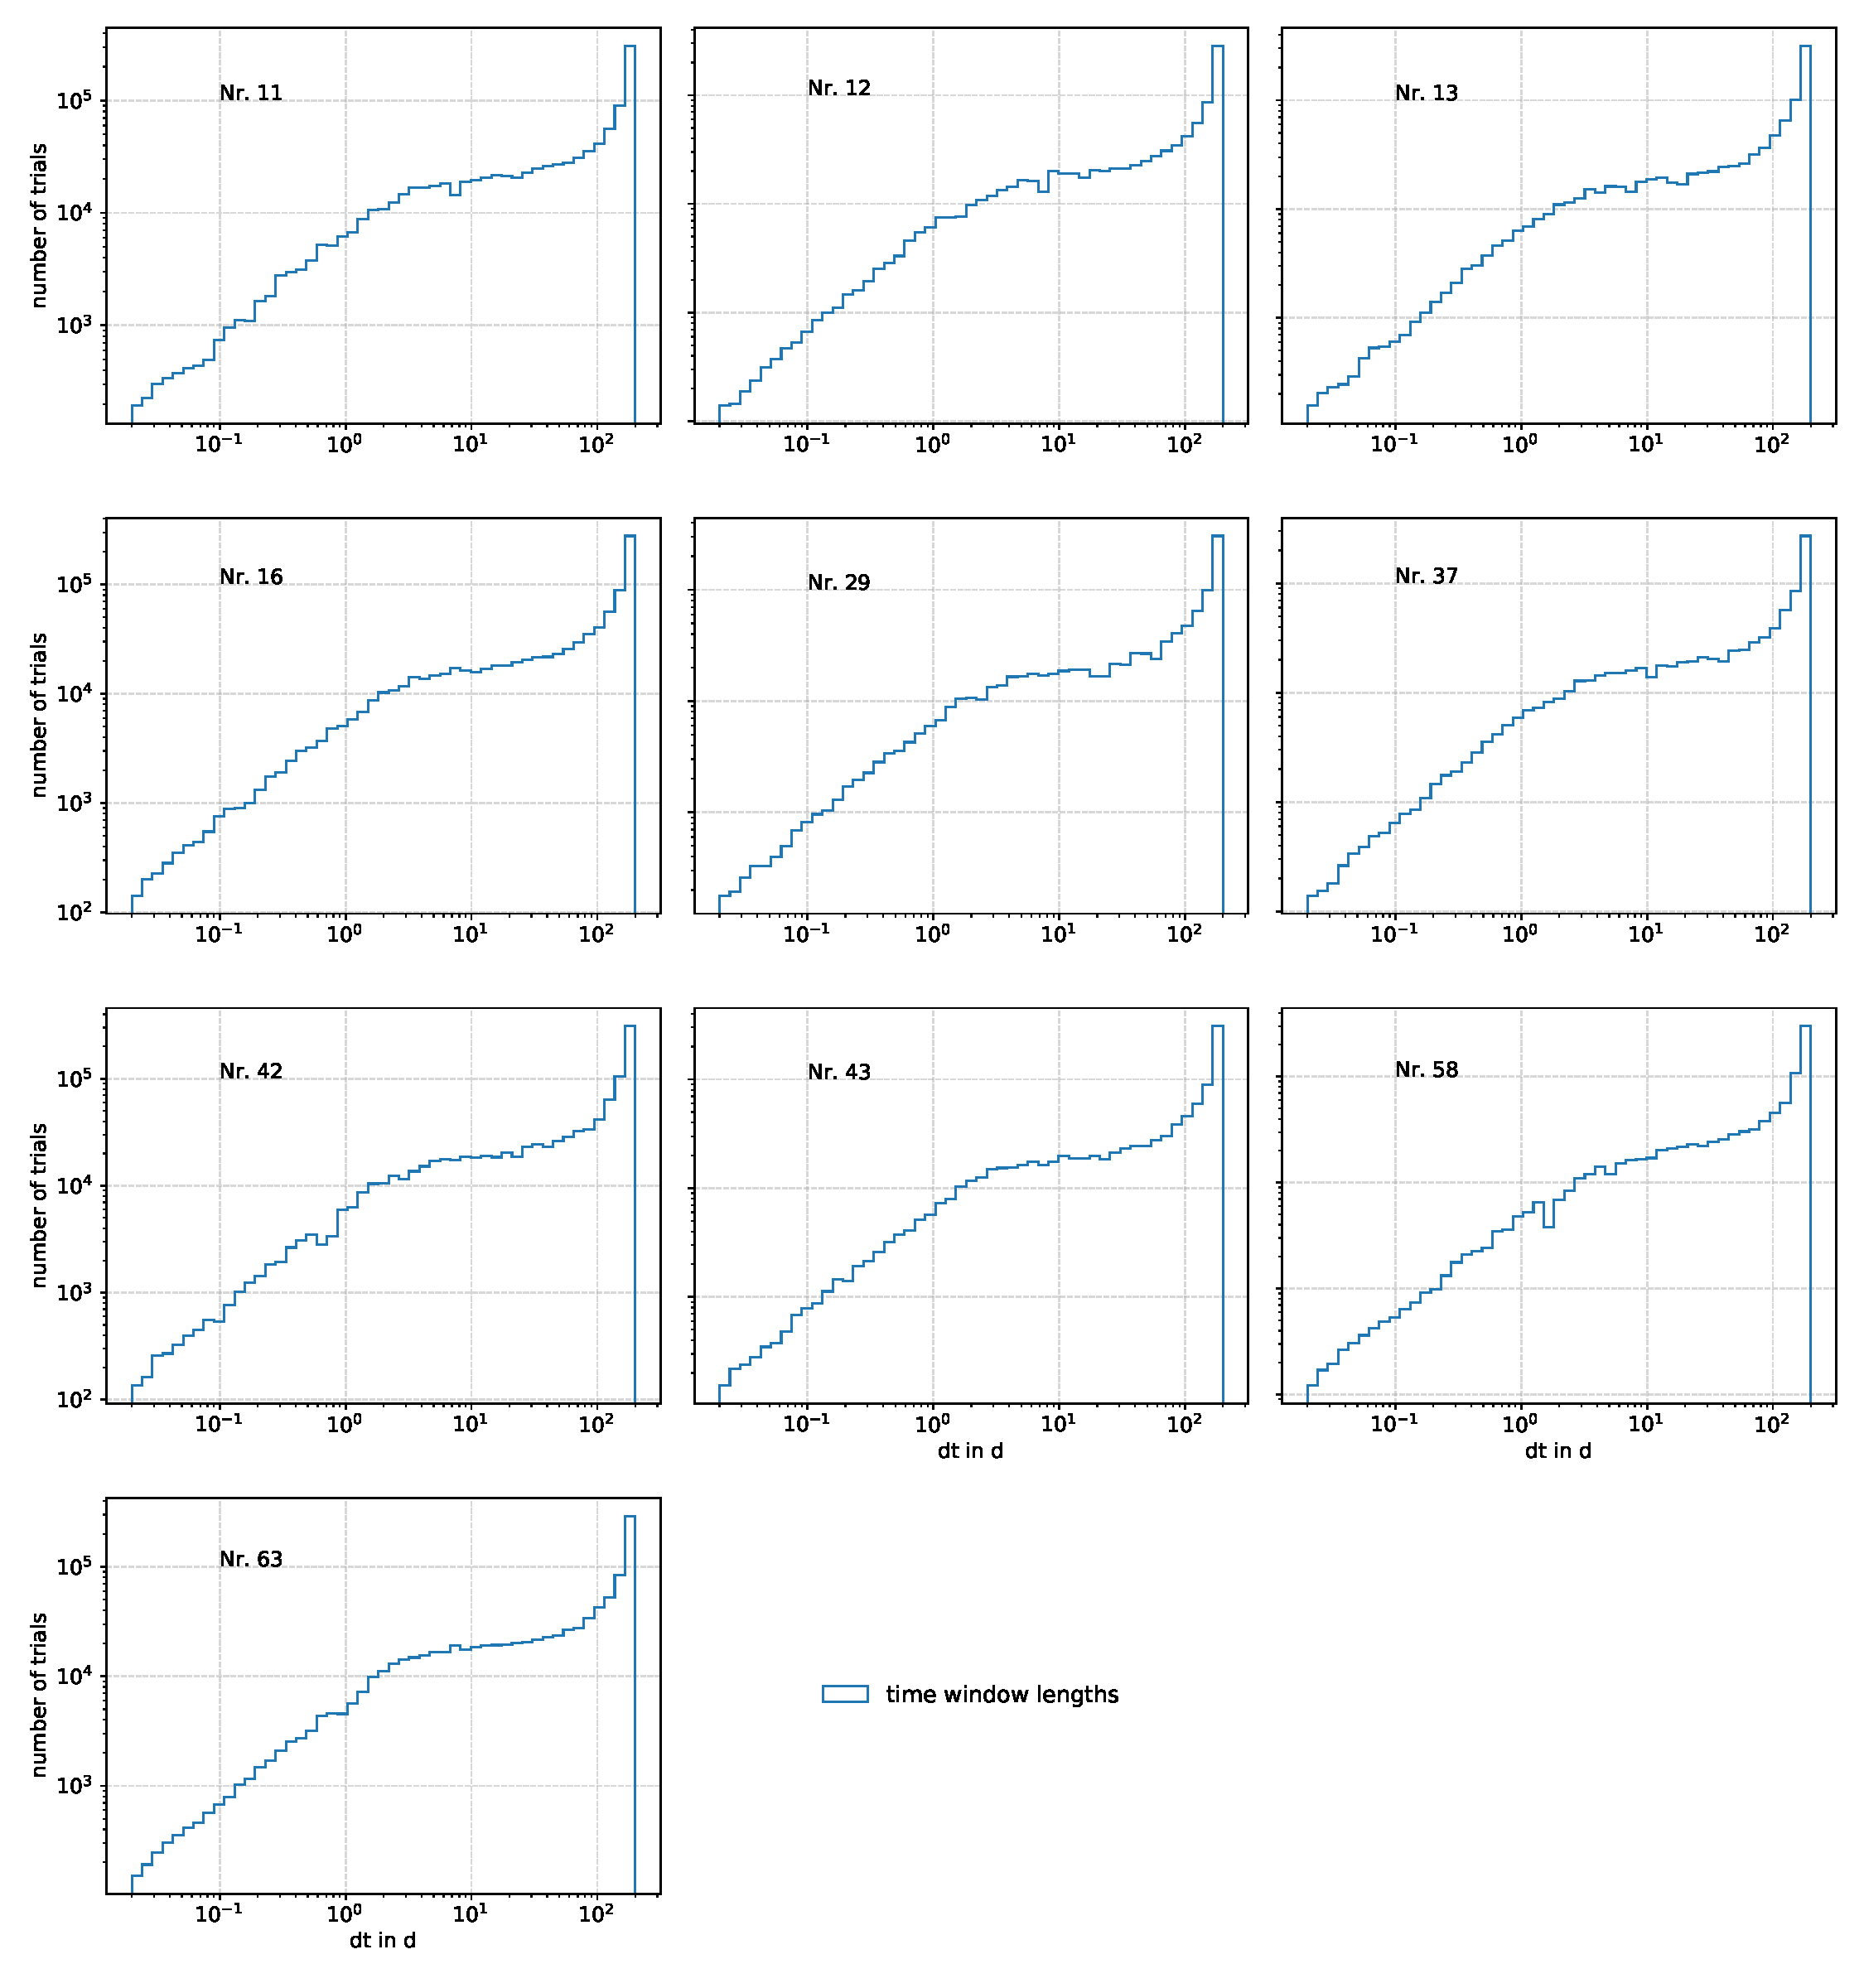
\includegraphics[width=\linewidth]{Plots/05_csky/9_years_gfu_gold_time_dep_bg_dt.pdf}
    \caption{Histograms of the background time window lengths $dt$ in days of all $\num{10}$ sources for the time-dependent analysis.}
    \label{fig:bg_trials_time_dep_time_windows}
\end{figure}

\begin{figure}
    \centering
    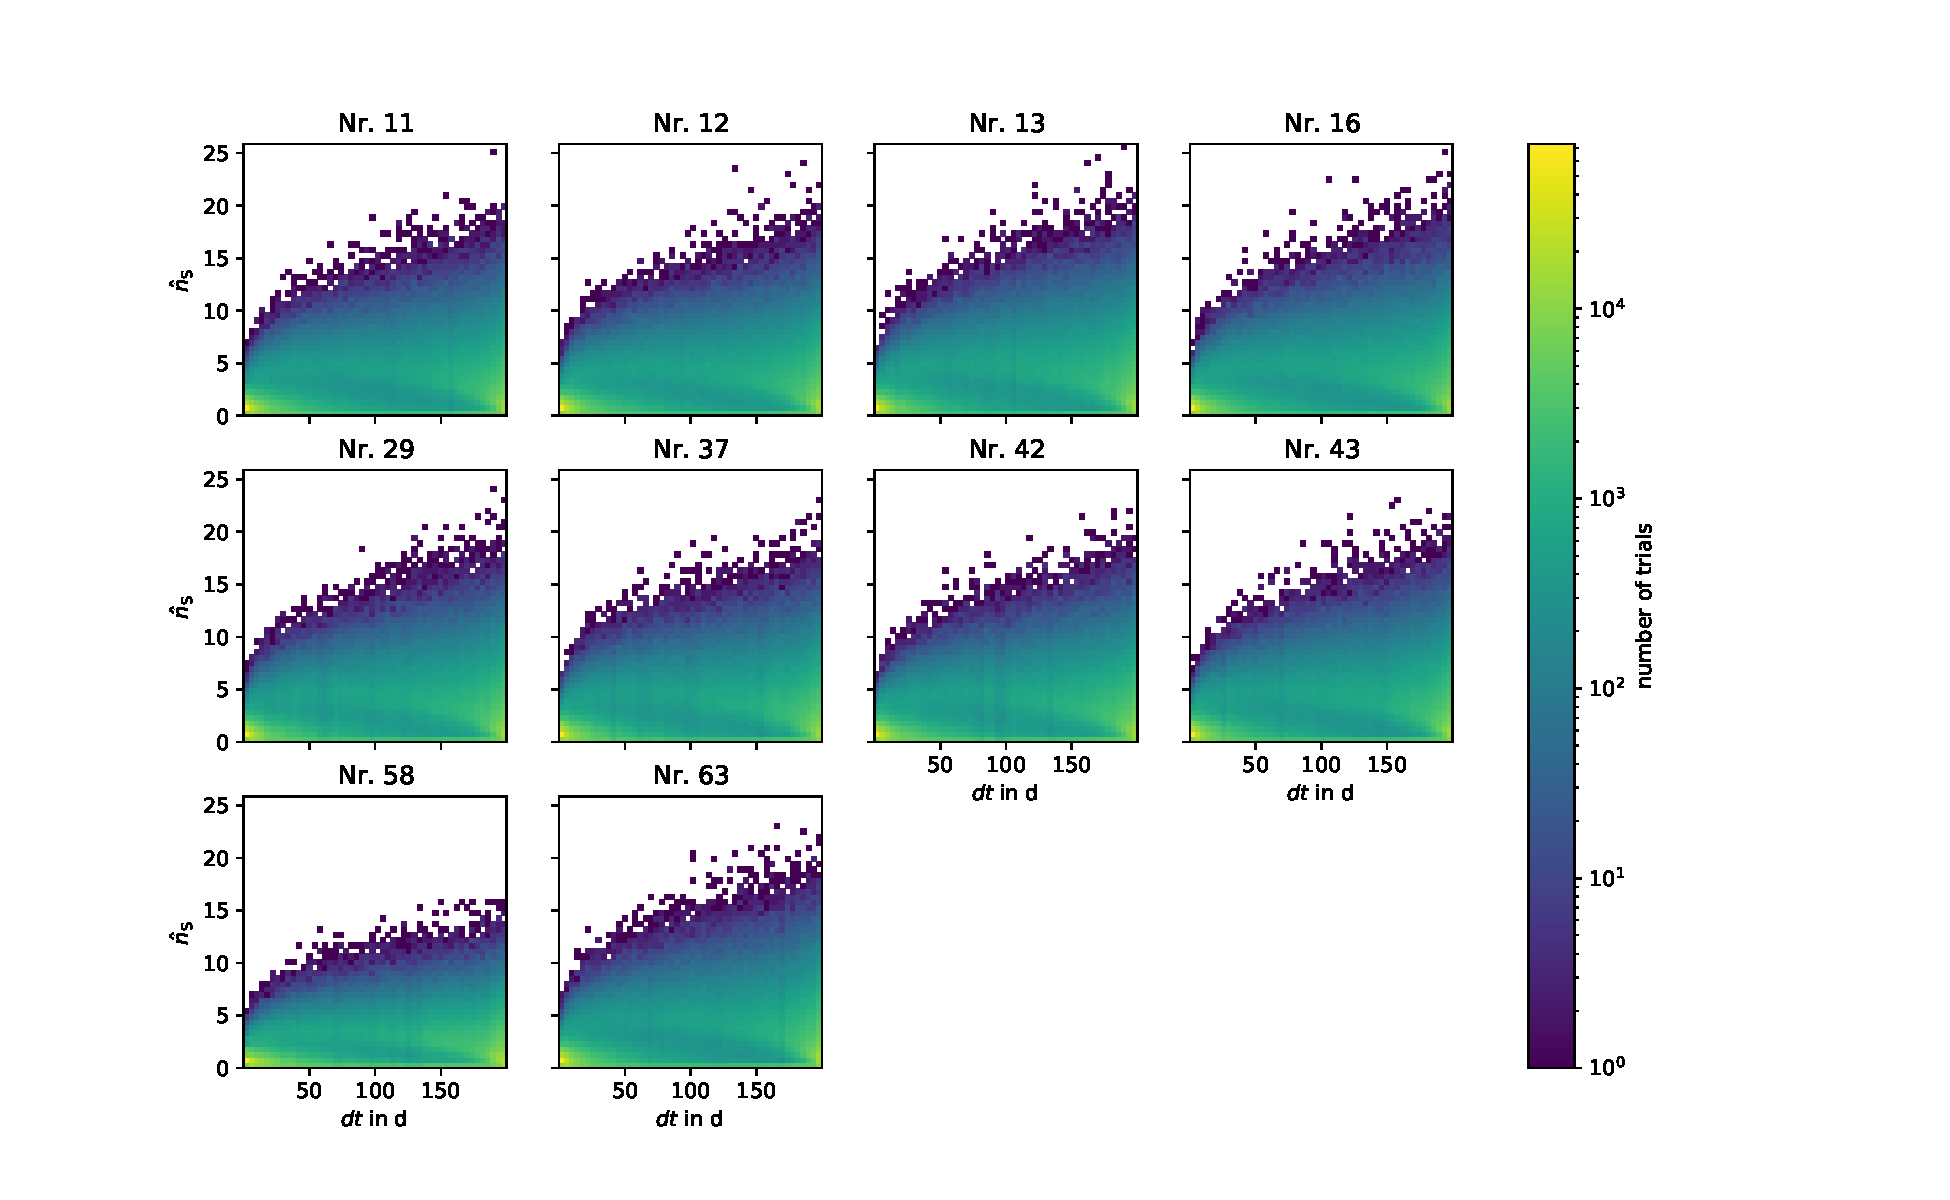
\includegraphics[width=\linewidth]{Plots/05_csky/time_window_ns_bg_time_dep.pdf}
    \caption{Histograms of the fitted number of signal events $\hat{n}_\text{S}$ in dependence of the time window lengths $dt$ in days of the background trials for the time-dependent analysis for all $\num{10}$ sources.}
    \label{fig:bg_trials_time_dep_time_windows_ns}
\end{figure}

\newpage
\subsection{Signal Trials}

\begin{table}
  \centering
  \caption{Table of the number of trials for each source index and number of injected signal events $n_\text{sig}$, running $\num{5}$ jobs with $\num{e4}$ trials per set of parameter pairs of source and $n_\text{sig}$. Some jobs fail due to technical reasons.}
  \label{tab:trials_sig_time_dep_table}
  \begin{tabular}{>{\centering\arraybackslash}p{.9cm}|%
                    cccccccccc}
    \toprule
    \: Nr. \newline $n_\text{sig}$ \: & 11 & 12 & 13 & 16 & 29 & 37 & 42 & 43 & 58 & 63 \\ 
    \toprule
    0.0 & 50000 & 50000 & 50000 & 50000 & 50000 & 10000 & 40000 & 50000 & 50000 & 30000 \\ 1.1 & 50000 & 50000 & 50000 & 50000 & 50000 & 20000 & 40000 & 50000 & 50000 & 20000 \\ 2.2 & 50000 & 50000 & 50000 & 50000 & 50000 & 0 & 40000 & 50000 & 50000 & 30000 \\ 3.3 & 50000 & 50000 & 40000 & 50000 & 50000 & 50000 & 40000 & 50000 & 50000 & 30000 \\ 4.4 & 50000 & 50000 & 30000 & 50000 & 50000 & 40000 & 50000 & 50000 & 50000 & 10000 \\ 5.6 & 50000 & 40000 & 30000 & 50000 & 50000 & 40000 & 50000 & 50000 & 50000 & 20000 \\ 6.7 & 50000 & 40000 & 30000 & 50000 & 50000 & 50000 & 50000 & 50000 & 50000 & 50000 \\ 7.8 & 50000 & 50000 & 30000 & 50000 & 50000 & 50000 & 50000 & 50000 & 50000 & 50000 \\ 8.9 & 50000 & 50000 & 30000 & 20000 & 40000 & 50000 & 50000 & 50000 & 50000 & 40000 \\ 10.0 & 50000 & 50000 & 30000 & 40000 & 50000 & 50000 & 50000 & 50000 & 50000 & 50000 \\ 12.0 & 50000 & 50000 & 50000 & 30000 & 50000 & 50000 & 50000 & 50000 & 50000 & 50000 \\ 14.0 & 50000 & 50000 & 50000 & 20000 & 50000 & 50000 & 50000 & 50000 & 50000 & 50000 \\ 16.0 & 50000 & 40000 & 50000 & 30000 & 50000 & 50000 & 50000 & 50000 & 50000 & 50000 \\ 18.0 & 50000 & 50000 & 50000 & 40000 & 50000 & 50000 & 50000 & 50000 & 50000 & 50000 \\ 20.0 & 50000 & 50000 & 50000 & 40000 & 50000 & 40000 & 50000 & 50000 & 50000 & 40000 \\ 22.0 & 50000 & 50000 & 50000 & 50000 & 50000 & 30000 & 50000 & 50000 & 50000 & 50000 \\ 24.0 & 50000 & 50000 & 50000 & 50000 & 50000 & 30000 & 50000 & 50000 & 50000 & 50000 \\ 26.0 & 50000 & 50000 & 50000 & 50000 & 50000 & 30000 & 50000 & 50000 & 50000 & 50000 \\ 28.0 & 50000 & 50000 & 50000 & 50000 & 50000 & 40000 & 50000 & 50000 & 50000 & 50000 \\ 30.0 & 50000 & 50000 & 50000 & 50000 & 30000 & 20000 & 50000 & 50000 & 50000 & 50000 \\ 
    \toprule
  \end{tabular}
\end{table}

\begin{figure}
    \centering
    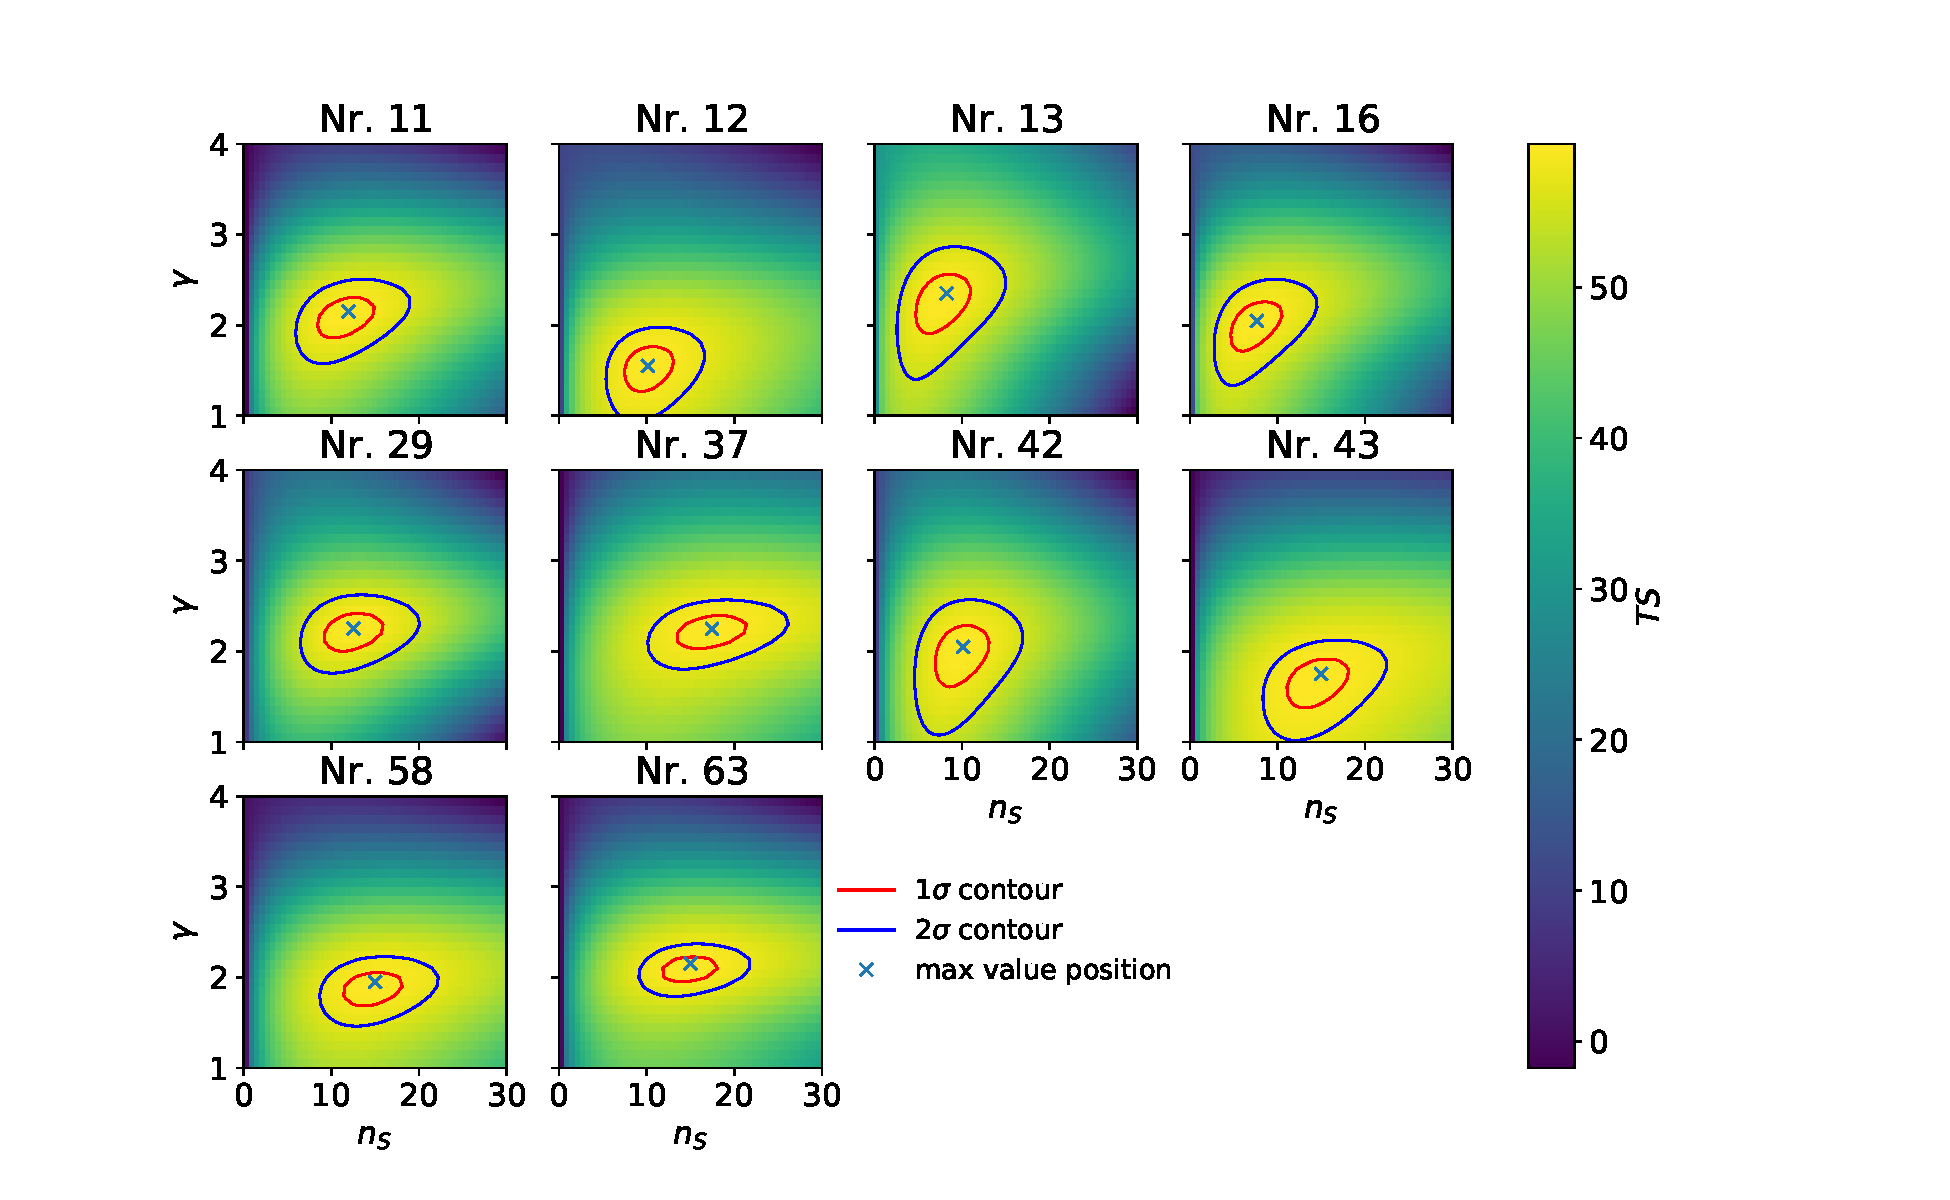
\includegraphics[width=\linewidth]{Plots/appendix/llh_scan.pdf}
    \caption{Scan of the likelihoodspace for all $\num{10}$ sources with a timewindow of $\SI{200}{\day}$ for the time-dependent analysis. The scan is in the spectral index $\gamma$ and the signal parameter $n_\text{S}$. The number of induced signal events is $n_S = \num{10}$ with a spectral index of $\gamma = 2$. The maximum test statistic value is marked in the plot including the contours of $\num{1}\sigma$ and $\num{2}\sigma$ and source number corresponds to table \ref{tab:sources}.}
    \label{fig:llh_scan_time_dep_all}
\end{figure}

\begin{figure}
    \centering
    \includegraphics[width=\linewidth]{Plots/appendix/9_years_gfu_gold_time_dep_cdf_sens.pdf}
    \caption{Quantiles of the signal trials for the calculation of the discovery potential for the time-dependent analysis of all $\num{10}$ sources at a spectral index of $\gamma=\num{2}$. A $\chi^2$ CDF fit provides a more accurate estimate of the sought signal parameter $n_\text{S}$ which satisfies the condition of the sensitivity at $\SI{90}{\percent}$ represented via a dashed line.}
    \label{fig:time_dep_cdf_sens}
\end{figure}

\begin{figure}
    \centering
    \includegraphics[width=\linewidth]{Plots/appendix/9_years_gfu_gold_time_dep_cdf_disc.pdf}
    \caption{Quantiles of the signal trials for the calculation of the discovery potential for the time-dependent analysis of all $\num{10}$ sources at a spectral index of $\gamma=\num{2}$. A $\chi^2$ CDF fit provides a more accurate estimate of the sought signal parameter $n_\text{S}$ which satisfies the condition of the discovery potential at $\SI{50}{\percent}$ represented via a dashed line.}
    \label{fig:time_dep_cdf_disc}
\end{figure}

\begin{figure}
    \centering
    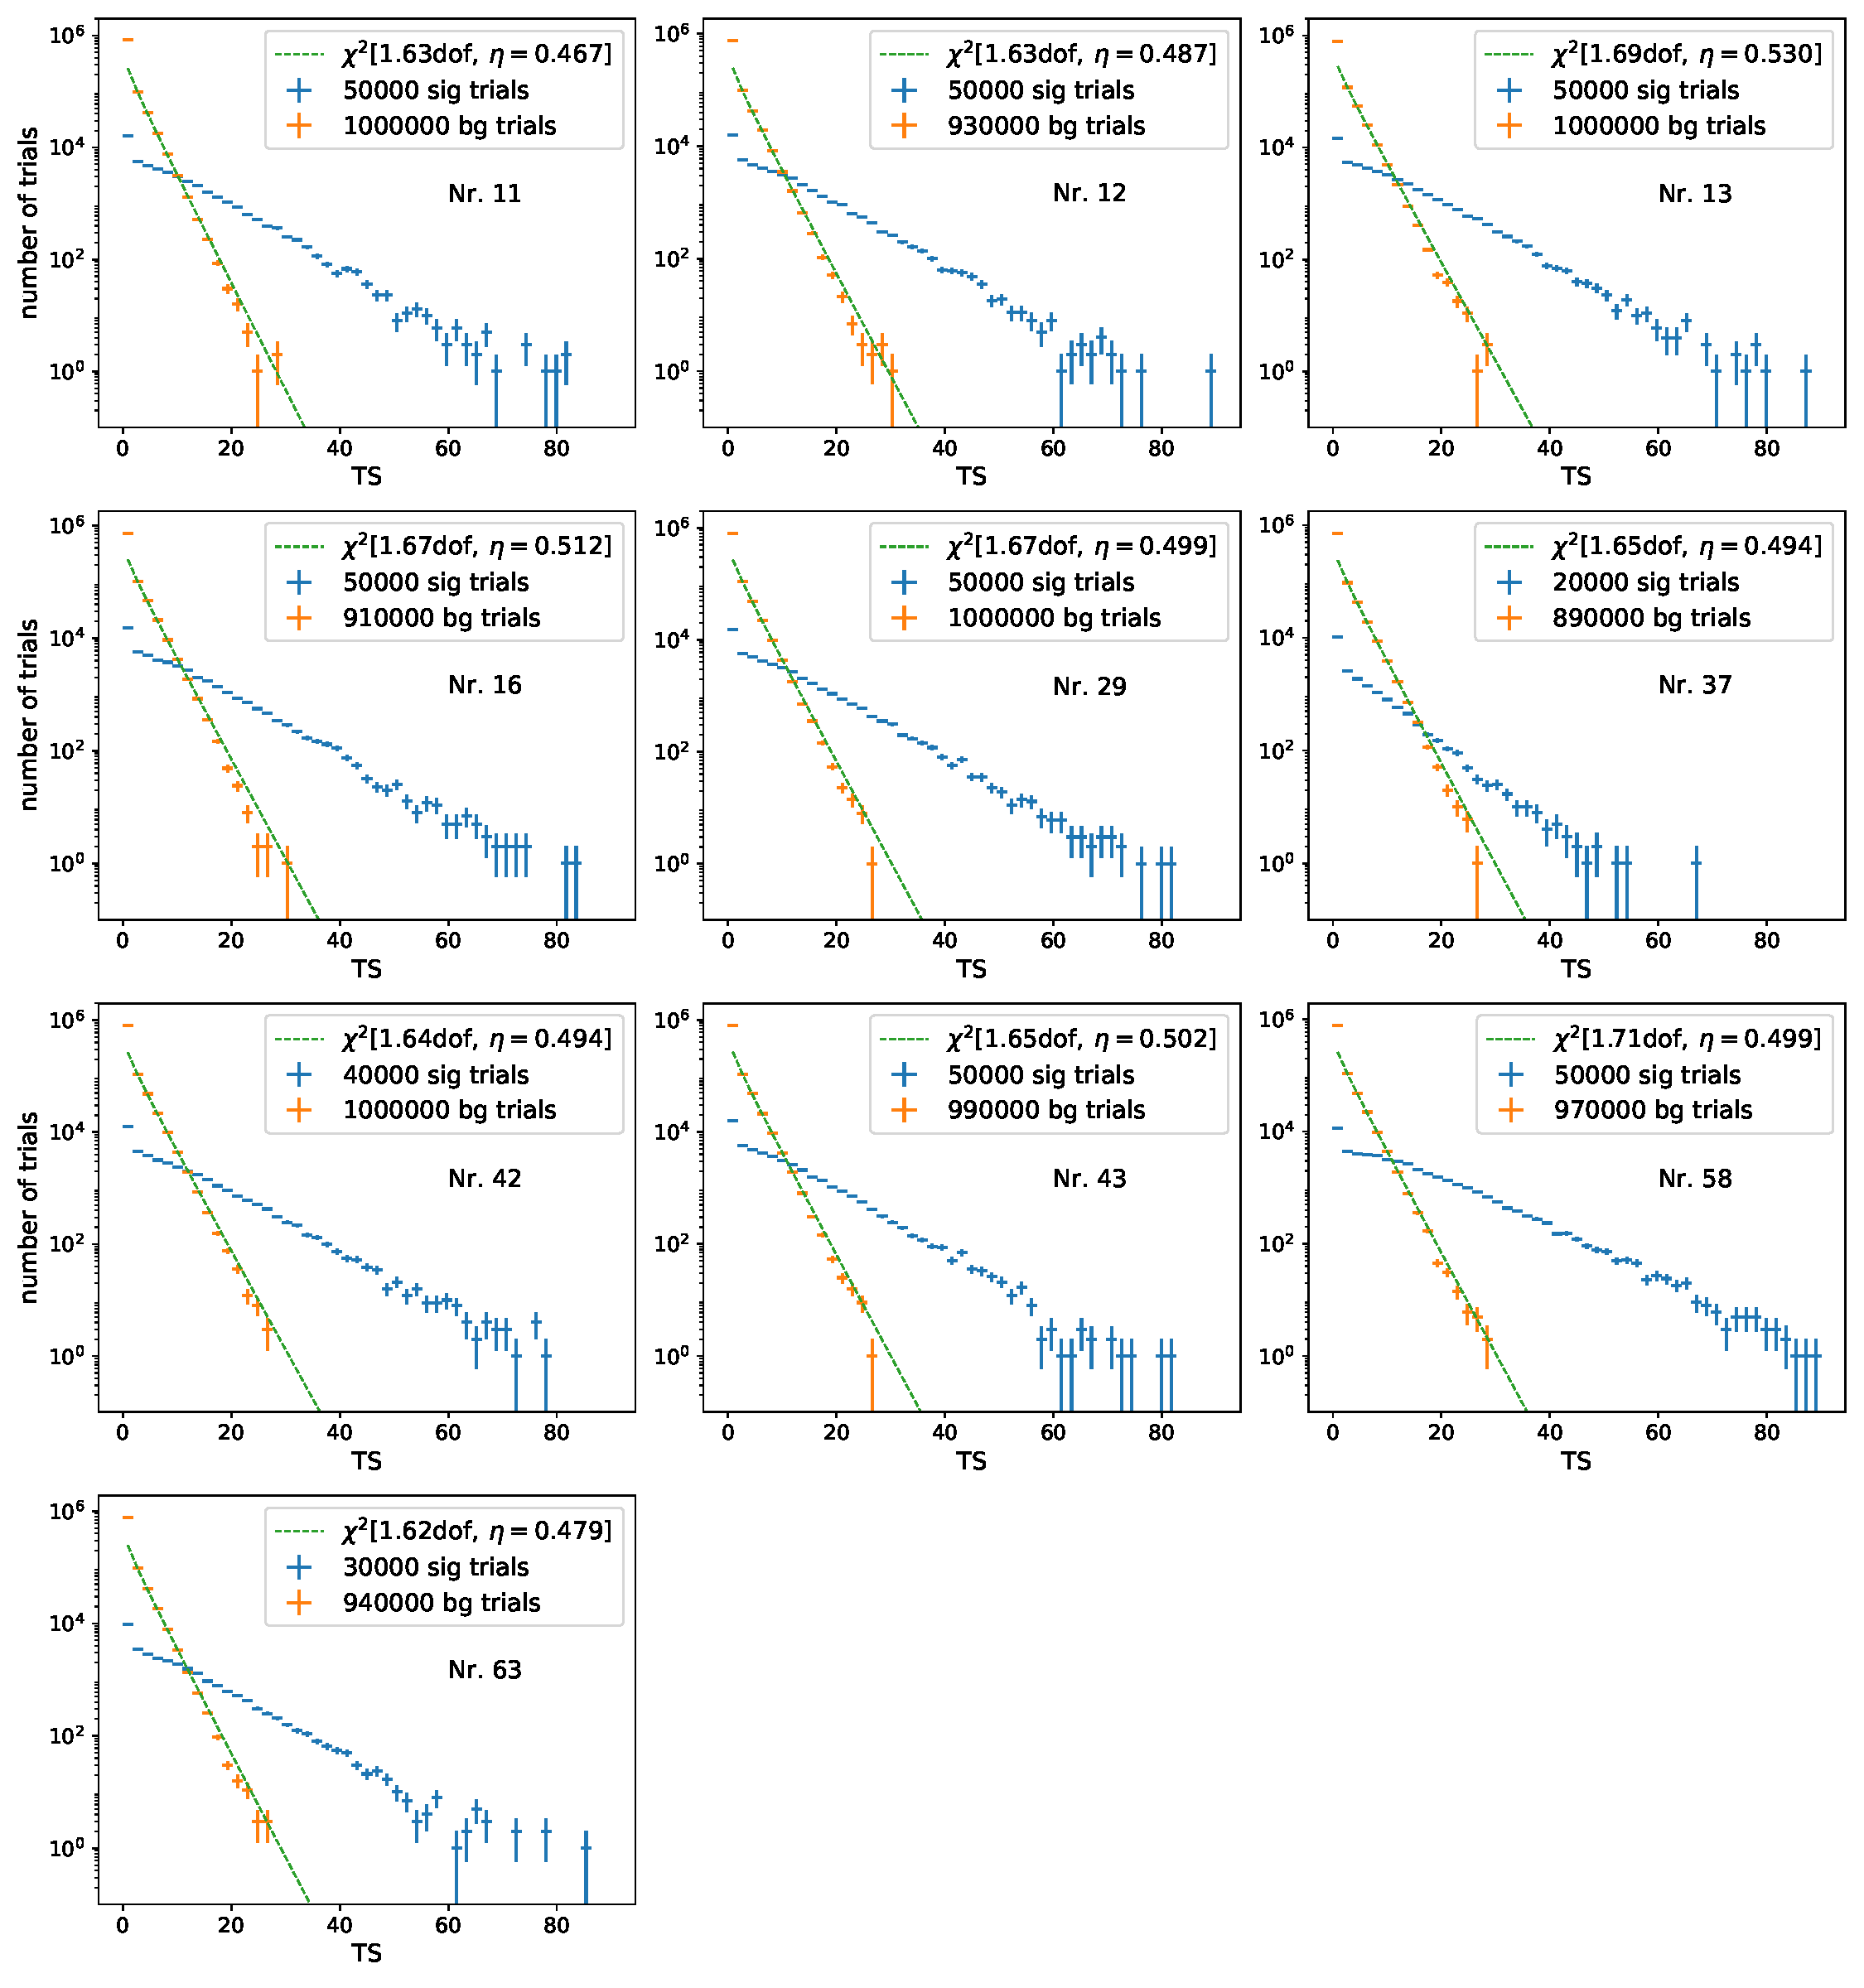
\includegraphics[width=\linewidth]{Plots/appendix/9_years_gfu_gold_time_dep_sig_sens_ts.pdf}
    \caption{Histogram of the background trials for the time-dependent analysis for all $\num{10}$ sources. Shown is also the set of signal trials with the number of injected signal events closest to satisfying the condition to calculate the sensitivity. The median of the background test statistics is not plotted as it is very close to the origin for all sources.}
    \label{fig:time_dep_sig_sens_ts}
\end{figure}

\begin{figure}
    \centering
    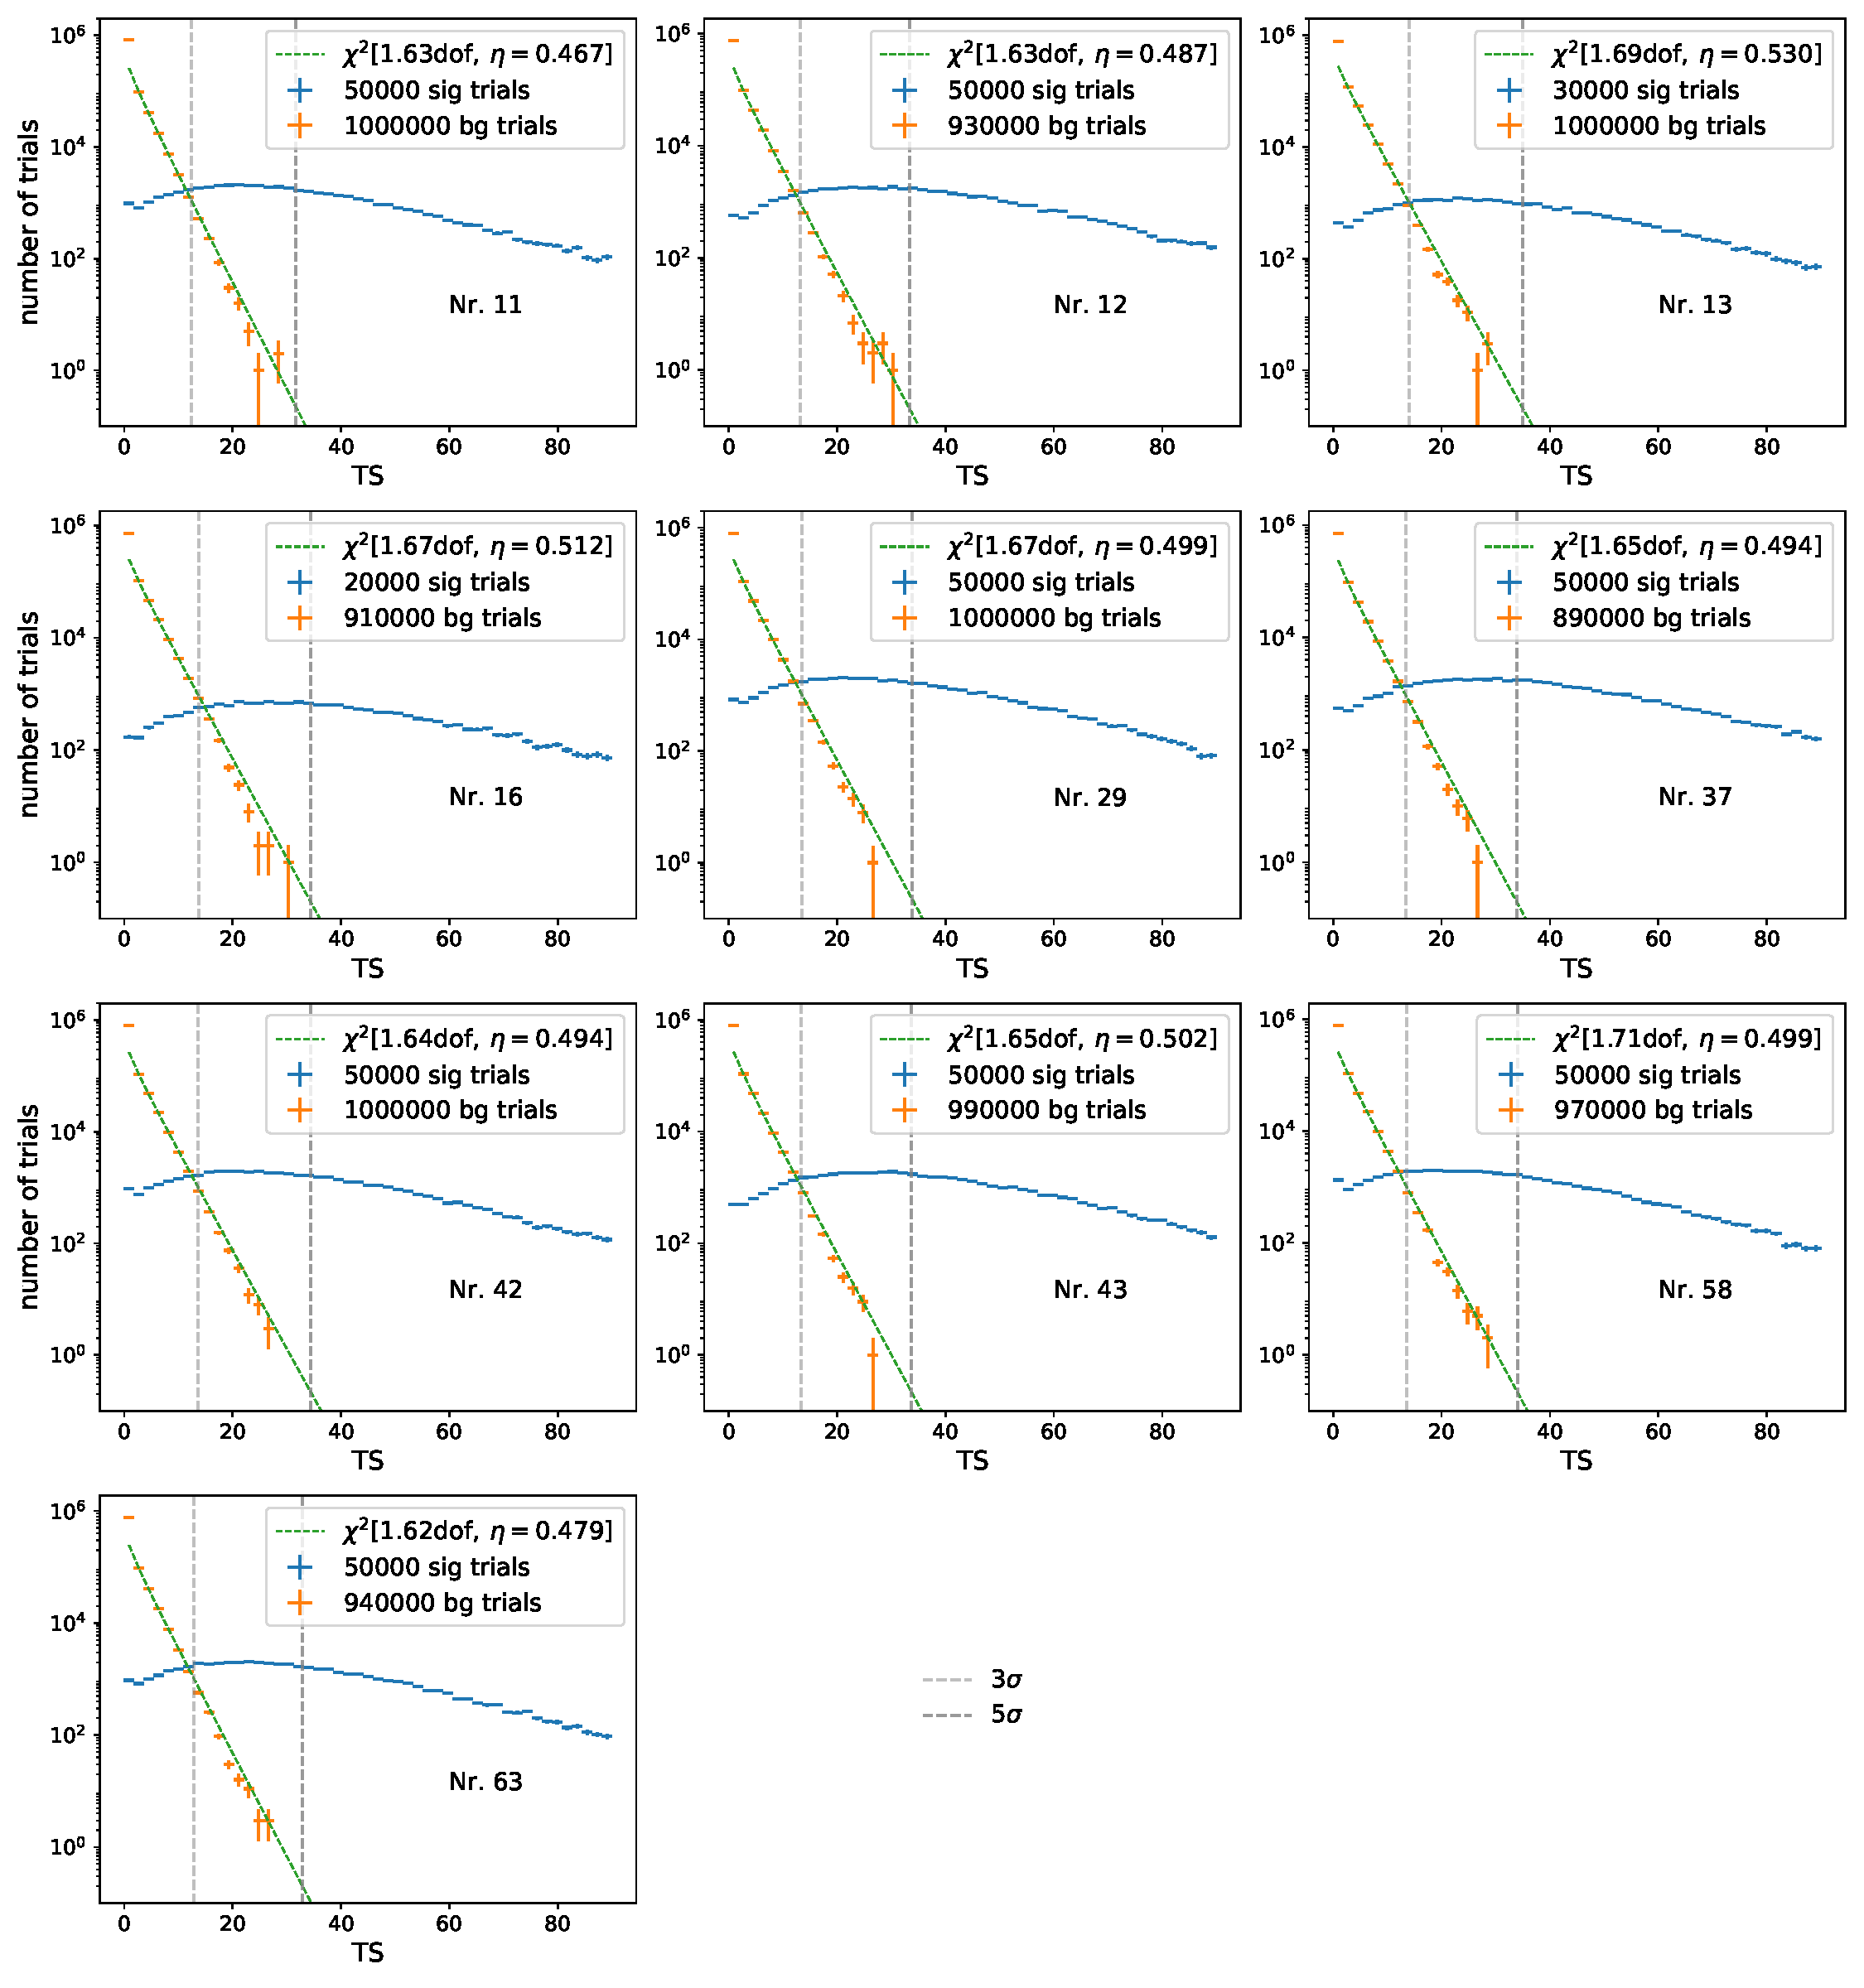
\includegraphics[width=\linewidth]{Plots/appendix/9_years_gfu_gold_time_dep_sig_disc_ts.pdf}
    \caption{Histogram of the background trials for the time-dependent analysis for all $\num{10}$ sources. Shown is also the set of signal trials with the number of injected signal events closest to satisfying the condition to calculate the discovery potential. The grey dashed lines represent $\num{3}\sigma$ and $\num{5}\sigma$ of the background teststatistic.}
    \label{fig:time_dep_sig_disc_ts}
\end{figure}

\begin{figure}
    \centering
    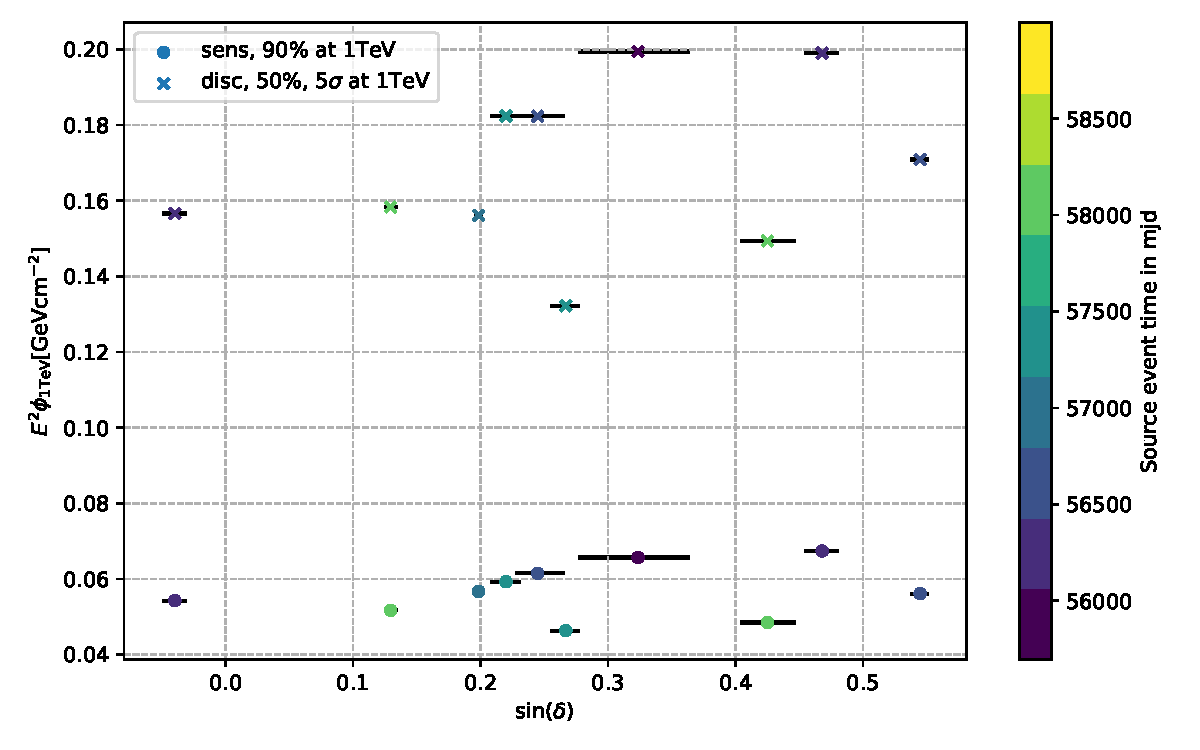
\includegraphics[width=\linewidth]{Plots/appendix/time_dep_sens_disc_dec_time_2.pdf}
    \caption{Sensitivities and discovery potentials for all $\num{10}$ sources in dependece of their position at a reference energy of $E_0 = \SI{100}{\tera\electronvolt}$ for the time-dependent analysis. The colour represents the arrival time of the source event and the errorbars the uncertainty in declination.}
    \label{fig:sens_disc_time_dep_dec}
\end{figure}

\begin{figure}
    \centering
    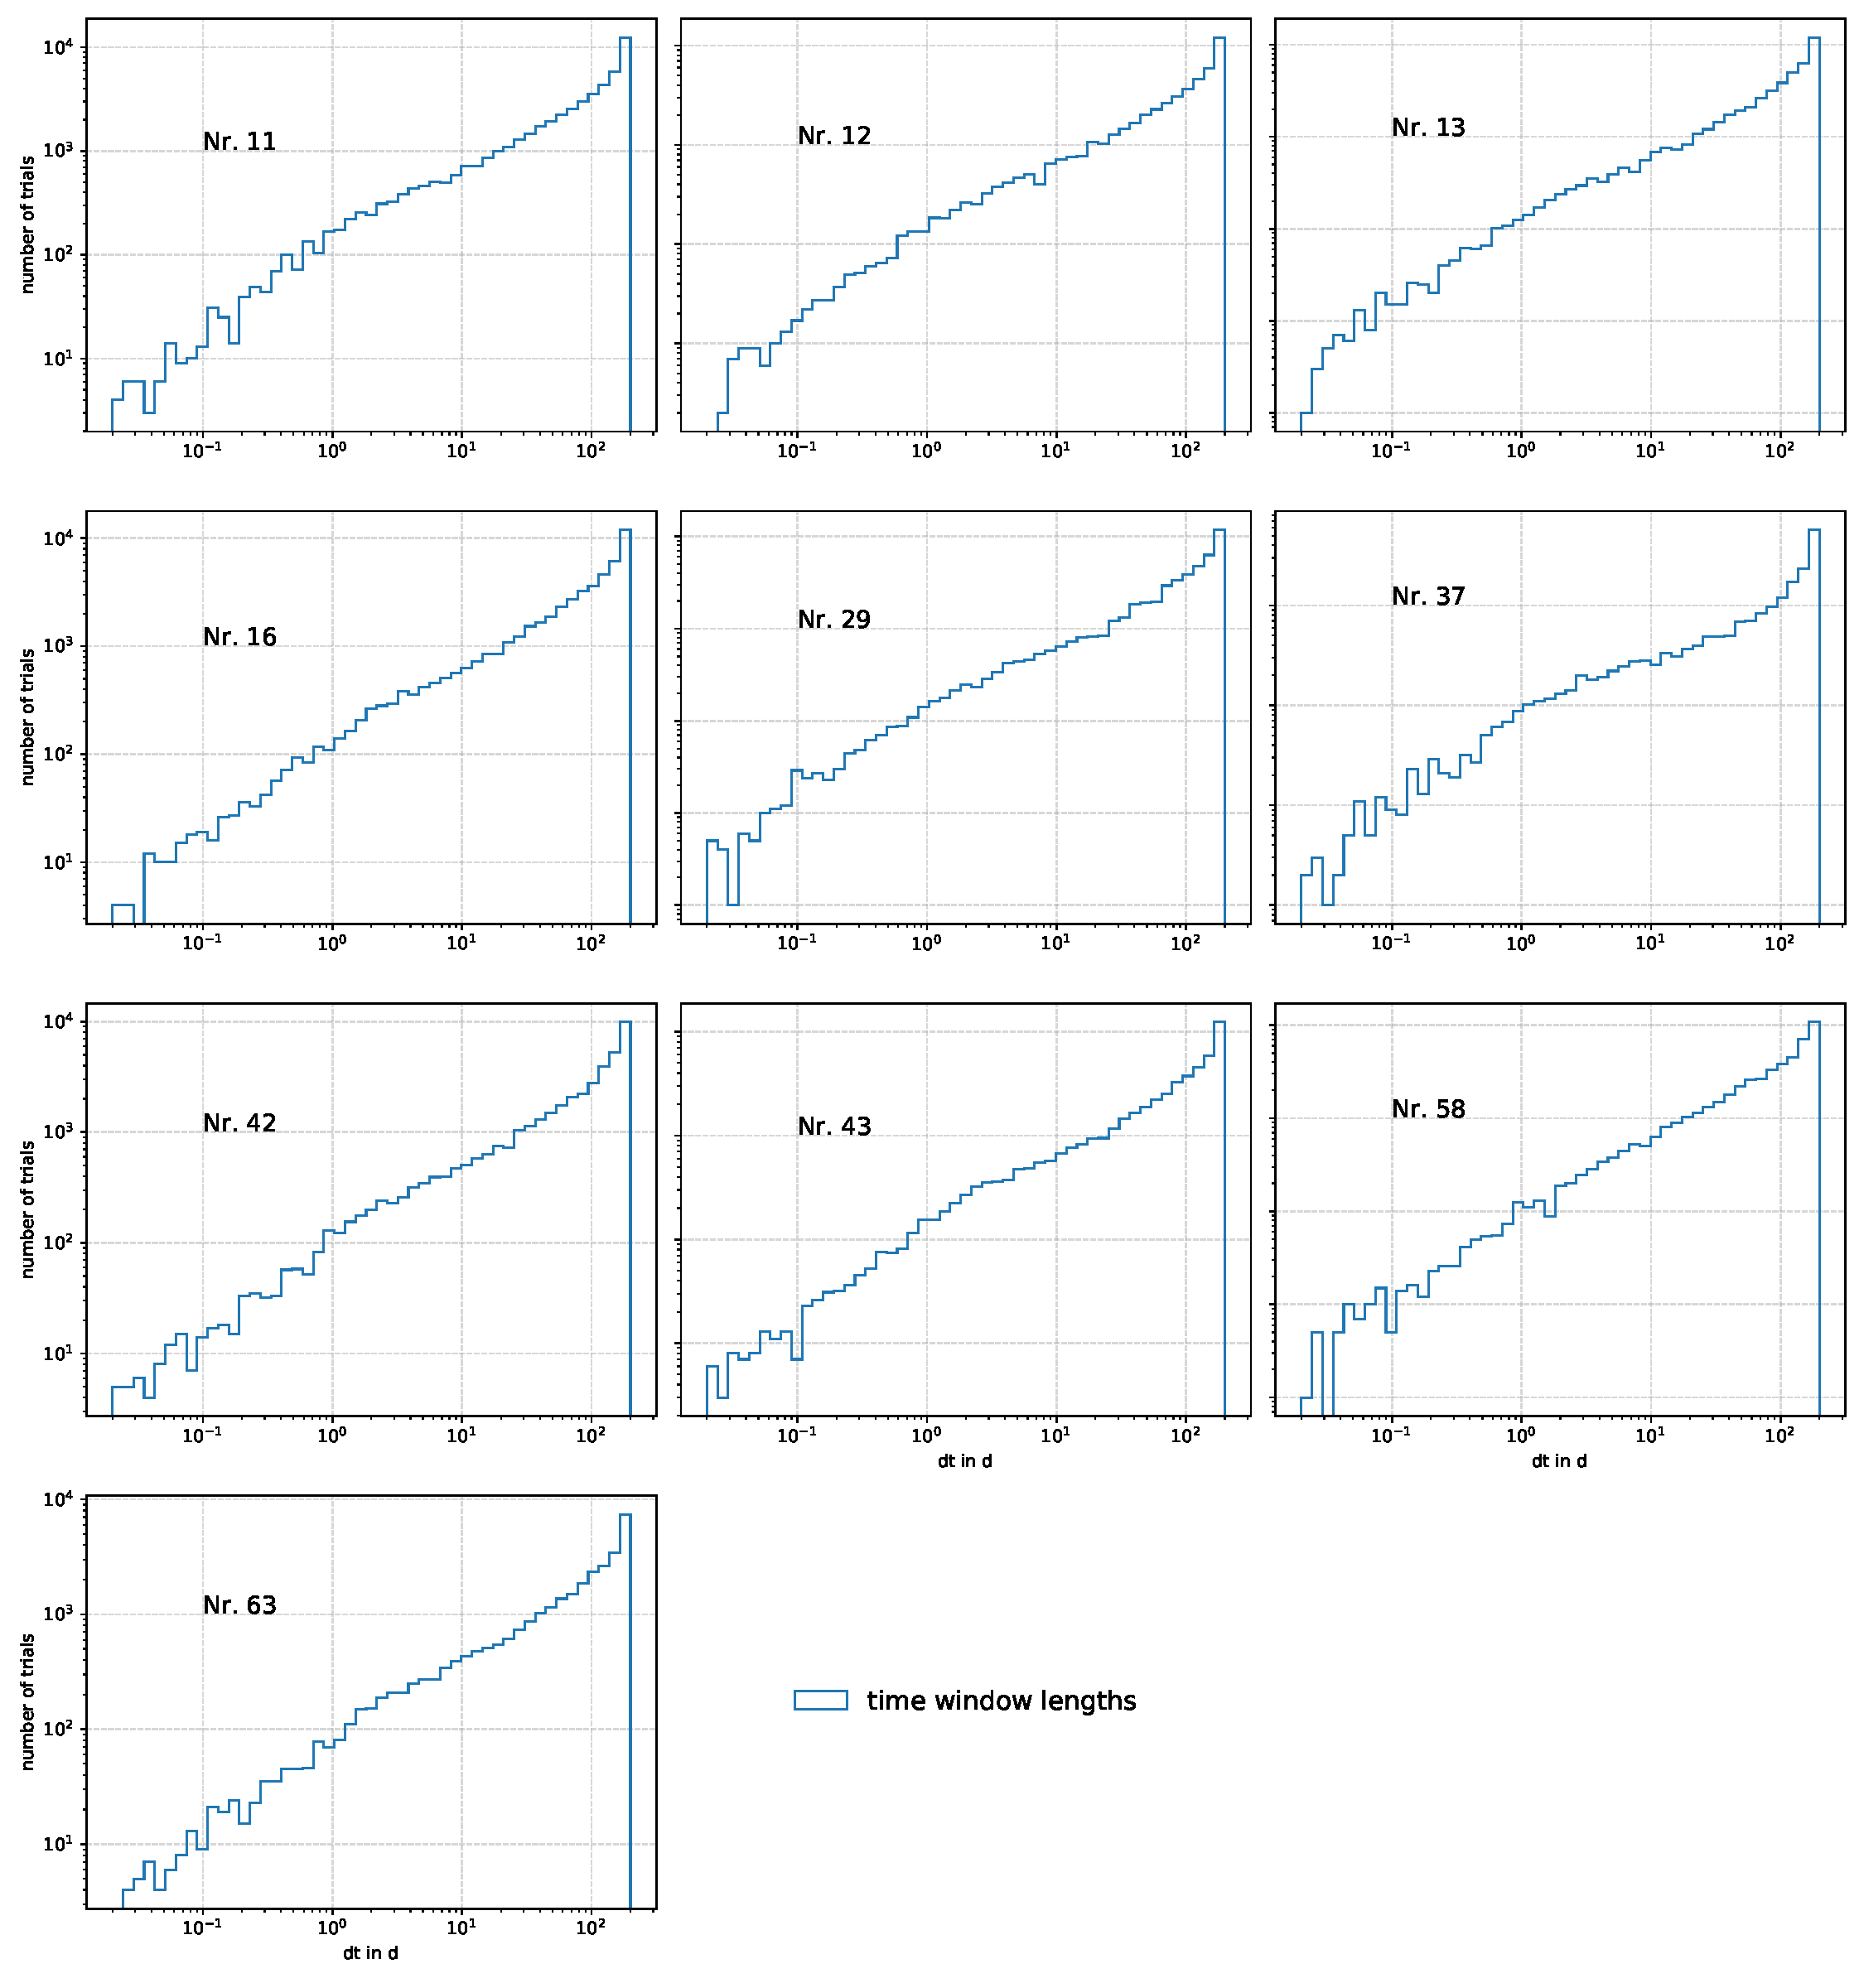
\includegraphics[width=\linewidth]{Plots/appendix/9_years_gfu_gold_time_dep_sens_dt.pdf}
    \caption{Histograms of the time window lengths $dt$ in days of all $\num{10}$ sources for the time-dependent analysis for the set of signal trials with the number of injected signal events closest to satisfying the condition to calculate the sensitivity.}
    \label{fig:sens_dt_all}
\end{figure}

\begin{figure}
    \centering
    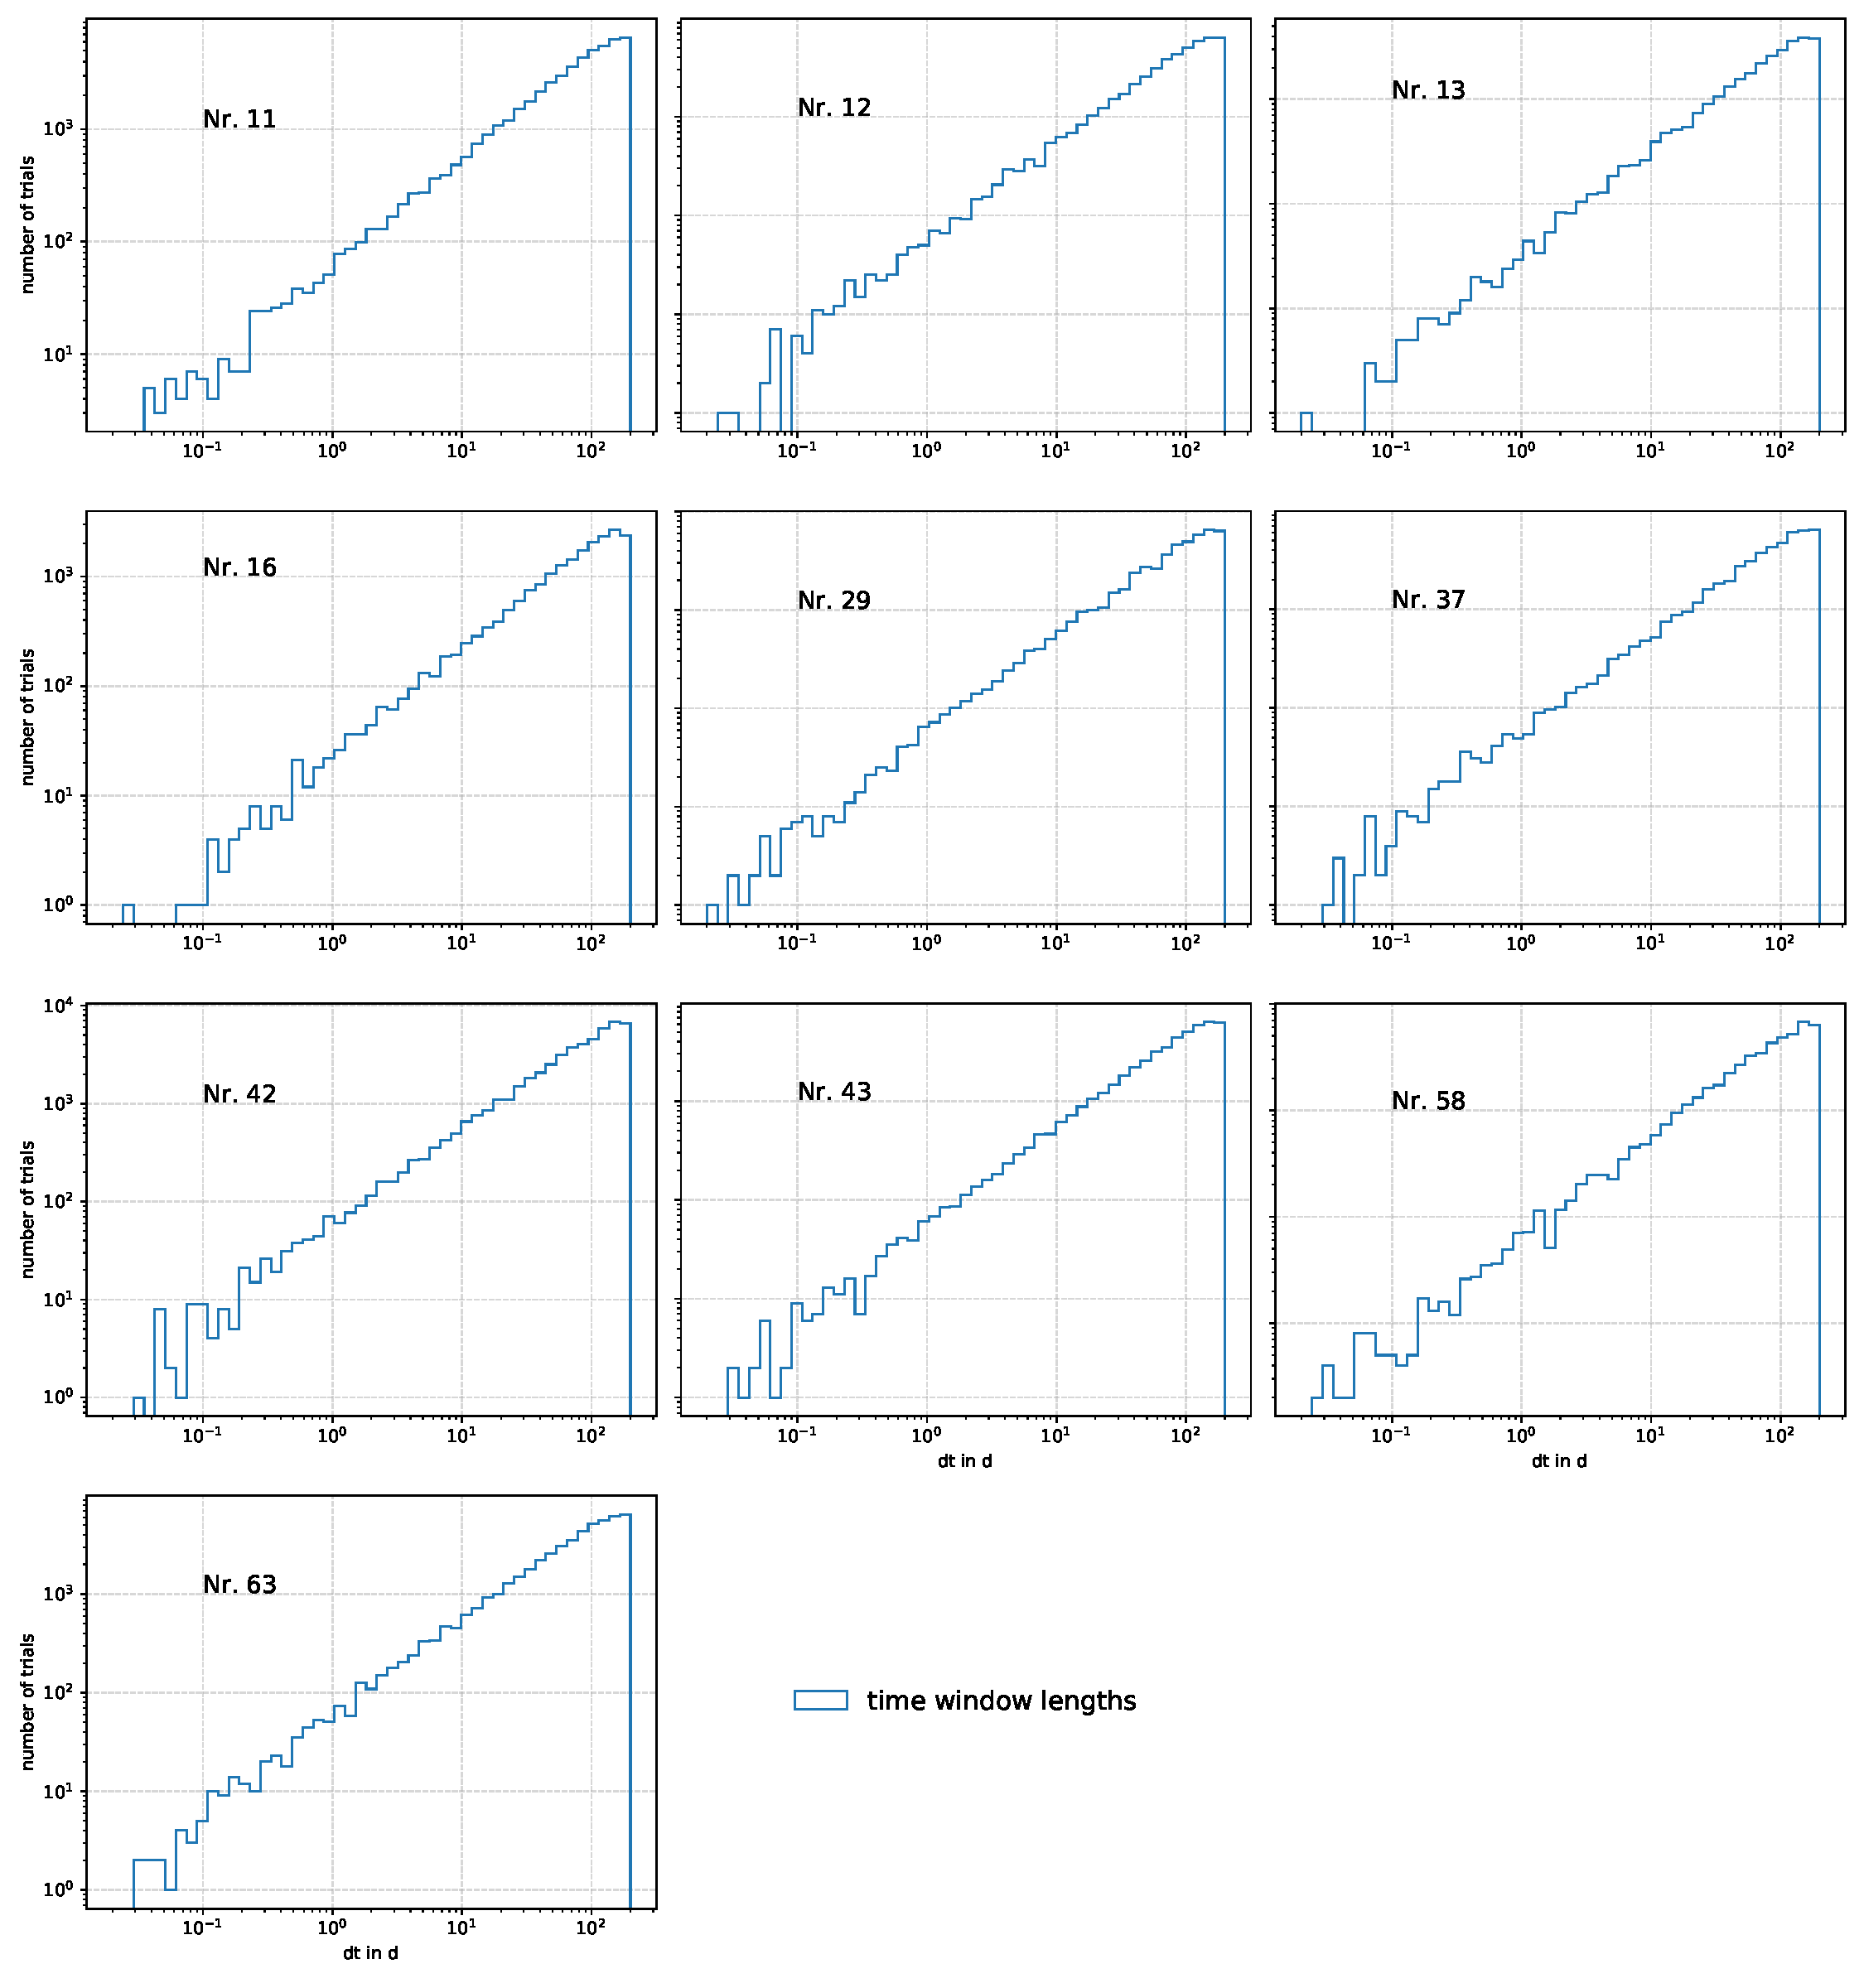
\includegraphics[width=\linewidth]{Plots/appendix/9_years_gfu_gold_time_dep_disc_dt.pdf}
    \caption{Histograms of the time window lengths $dt$ in days of all $\num{10}$ sources for the time-dependent analysis for the set of signal trials with the number of injected signal events closest to satisfying the condition to calculate the discovery potential.}
    \label{fig:disc_dt_all}
\end{figure}

\begin{figure}
    \centering
    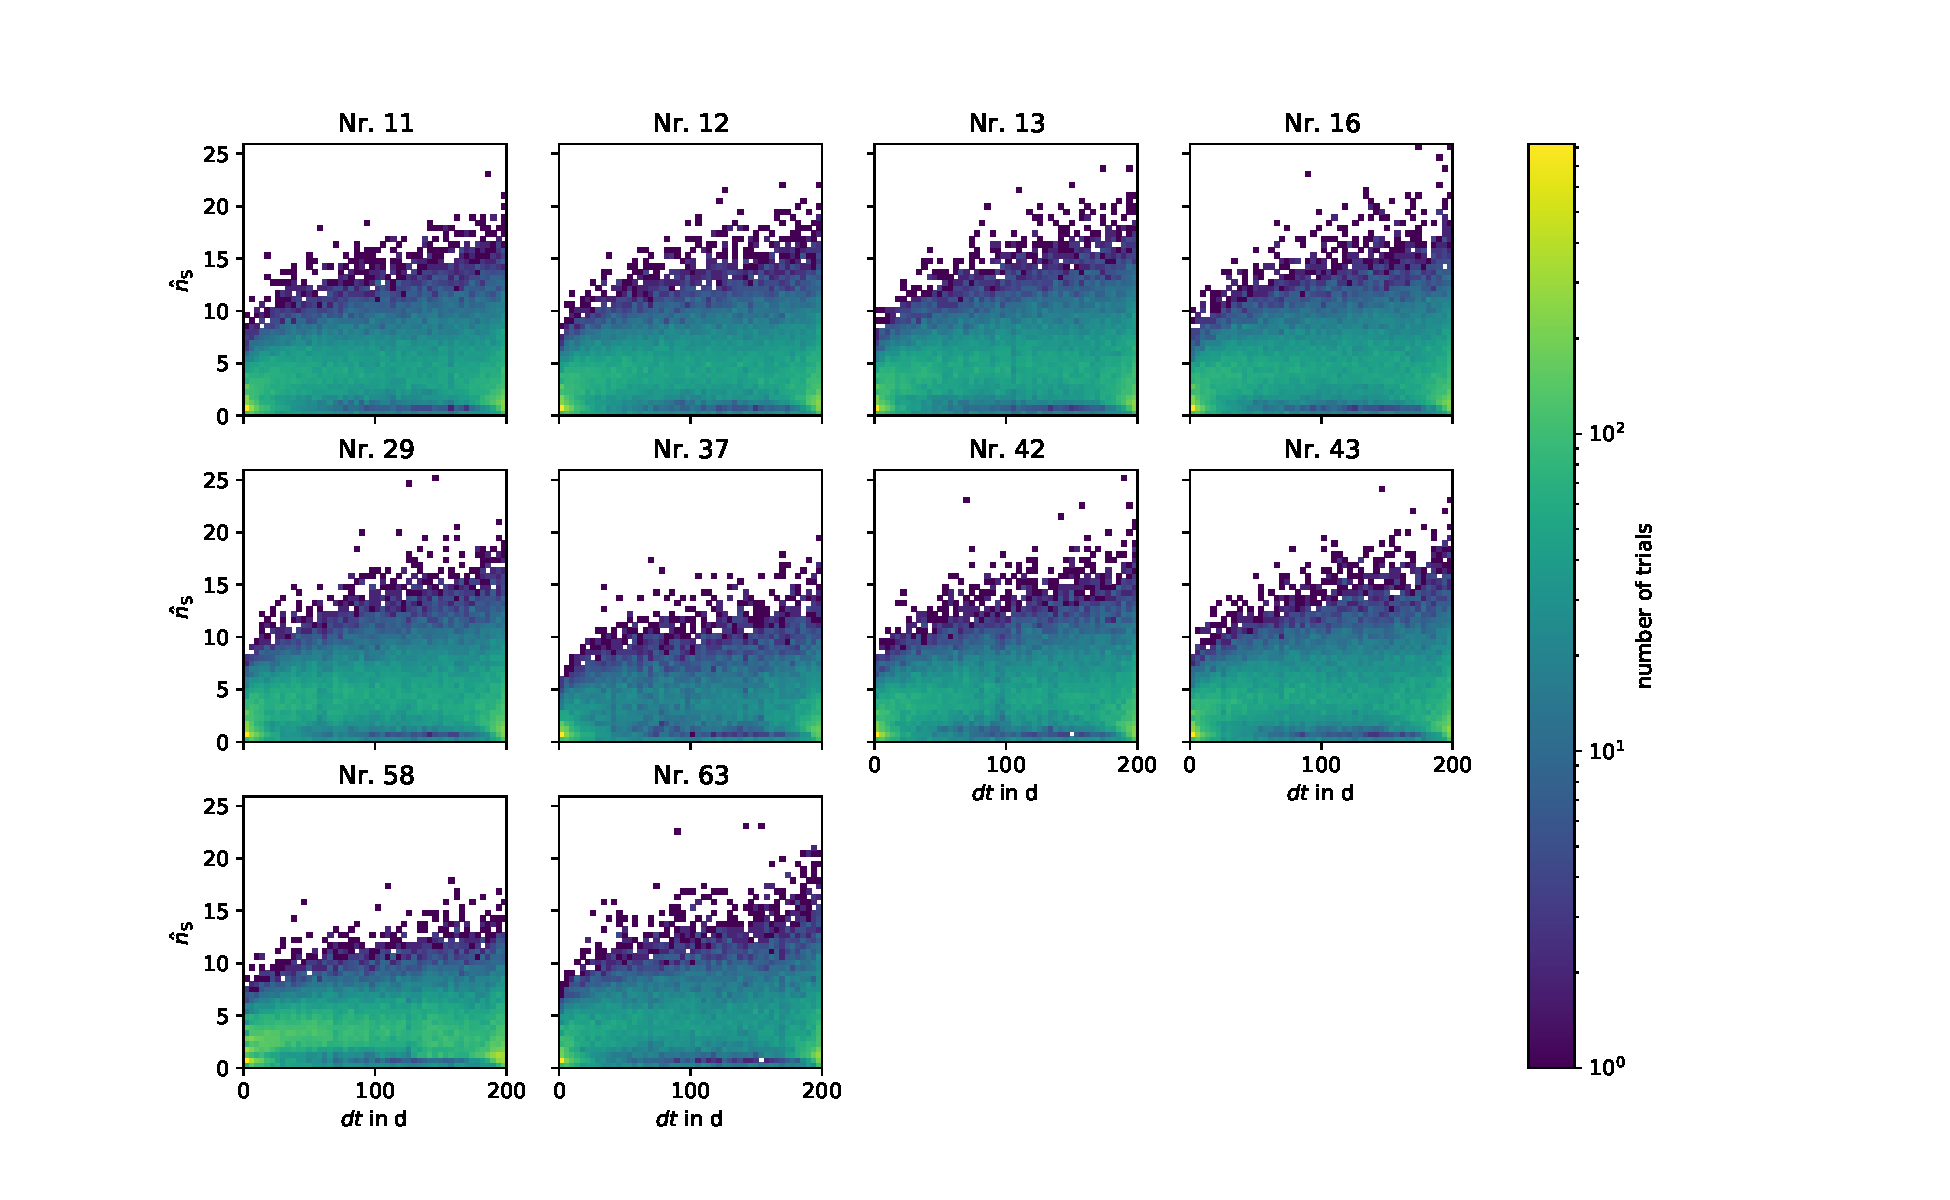
\includegraphics[width=\linewidth]{Plots/appendix/time_window_ns_sens_time_dep.pdf}
    \caption{Histograms of the time window lengths $dt$ in days in dependence of the fitted signal parameter $\hat{n}_\text{S}$ of all $\num{10}$ sources for the time-dependent analysis for the set of signal trials with the number of injected signal events closest to satisfying the condition to calculate the sensitivity.}
    \label{fig:sens_ns_dt_all}
\end{figure}

\begin{figure}
    \centering
    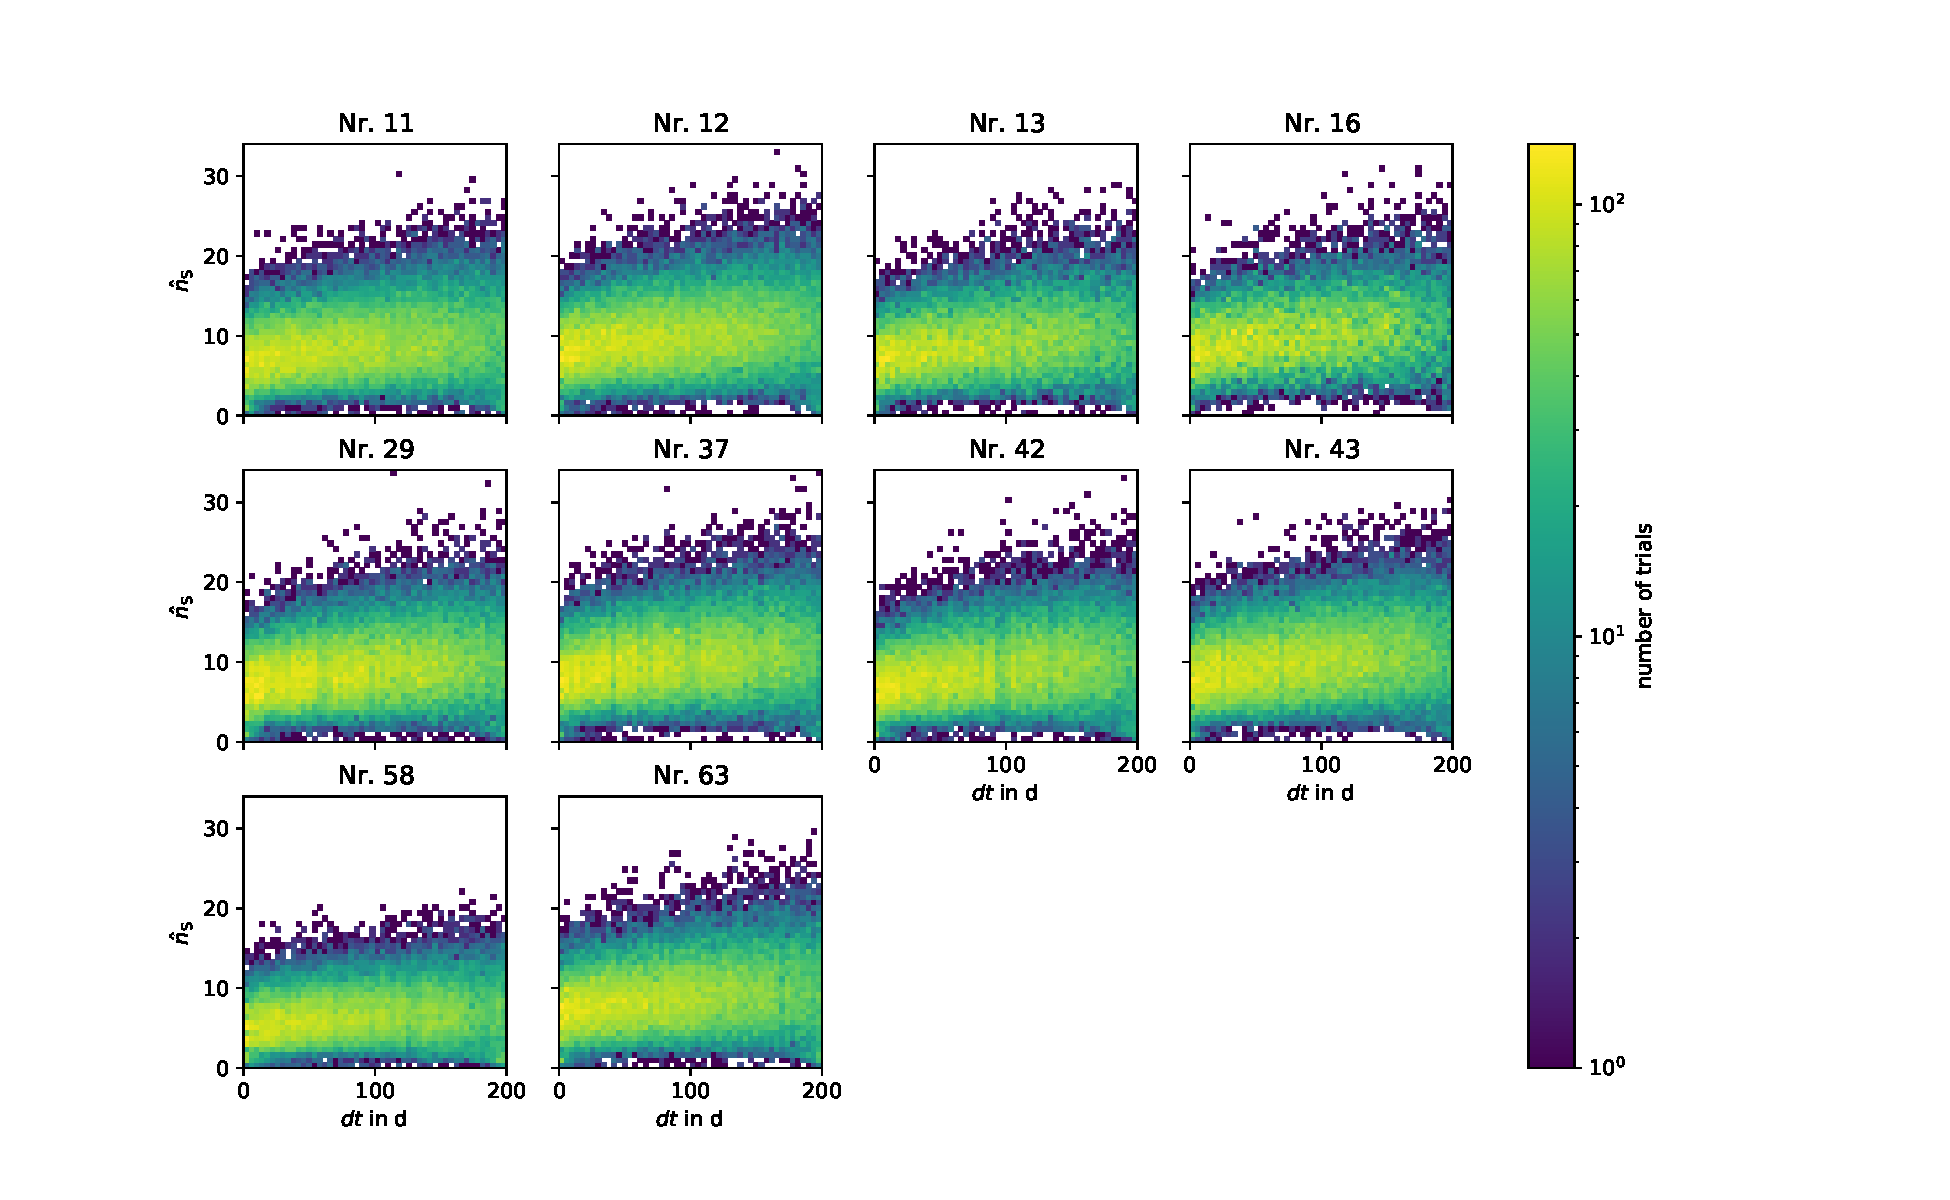
\includegraphics[width=\linewidth]{Plots/appendix/time_window_ns_disc_time_dep.pdf}
    \caption{Histograms of the time window lengths $dt$ in days in dependence of the fitted signal parameter $\hat{n}_\text{S}$ of all $\num{10}$ sources for the time-dependent analysis for the set of signal trials with the number of injected signal events closest to satisfying the condition to calculate the discovery potential.}
    \label{fig:disc_ns_dt_all}
\end{figure}

\newpage
\subsection{Examination of Fit Bias} \label{sec:fit_bias_time_dep}

\begin{figure}
    \centering
    \includegraphics[width=\linewidth]{Plots/appendix/gamma_fit_time_dep.pdf}
    \caption{Fitted spectral index $\hat\gamma$ in dependence of the injected number of signal events $n_\text{inj}$ with spectral index $\gamma$, shown with a horizontal black dashed line, for the trials used in the time-dependent analysis.}
    \label{fig:gamma_fit_time_dep}
\end{figure}

\begin{figure}
    \centering
    \includegraphics[width=\linewidth]{Plots/appendix/ns_fit_time_dep.pdf}
    \caption{Fitted number of signal events $\hat{n}_{\text{S}}$ in dependence of the injected number of signal events $n_\text{inj}$ with spectral index $\gamma$ for the time-dependent analysis. The black dashed line shows the equality of fitted and injected number of signal events.}
    \label{fig:ns_fit_time_dep}
\end{figure}

\section{Time-Dependent Stacking Software Approach}

This chapter contains additional understanding aids for the attempt to write software for point source searches.

\begin{figure}
  \scalebox{0.5}{
  \begin{tikzpicture}[scale=1]
    \node[draw] at (-10,2.5) {\includegraphics[width=4cm]{Plots/appendix/example.png}};
    % Koordinatensystem
    \draw[line width=0.25mm, ->] (-5,0) -- (-5,5);
    \draw[line width=0.25mm, ->] (-5,0) -- (10,0);
    \node at (10,-0.5) {time};
    \node at (-5.5,3) {rate};
    % Quellen
    \draw[line width=0.5mm, green] (-1,-1) -- (-1,4);
    \fill[pattern = north east lines, pattern color = green, opacity = 0.5,domain=-3:1,variable=\x]
    (-3,0)
    -- plot ({\x},{3.5})
    -- (1,0)
    -- cycle;
    \fill[pattern = north east lines, pattern color = green, opacity = 0.5,domain=-3:1,variable=\x]
    (-3,0)
    -- plot ({\x},{-0.5})
    -- (1,0)
    -- cycle;
    \draw[green] (-3,-0.5) -- (1,-0.5);
    \draw[green] (-3,3.5) -- (1,3.5);
    \draw[green] (-3,-0.5) -- (-3,3.5);
    \draw[green] (1,-0.5) -- (1,3.5);
    \node[green] at (-1,4.5) {$k=1$};

    \draw[line width=0.5mm, orange] (-0.8,-1) -- (-0.8,4);
    \fill[pattern = north east lines, pattern color = orange, opacity = 0.5,domain=-2.8:1.2,variable=\x]
    (-2.8,0)
    -- plot ({\x},{3.5})
    -- (1.2,0)
    -- cycle;
    \fill[pattern = north east lines, pattern color = orange, opacity = 0.5,domain=-2.8:1.2,variable=\x]
    (-2.8,0)
    -- plot ({\x},{-0.5})
    -- (1.2,0)
    -- cycle;
    \draw[orange] (-2.8,-0.5) -- (1.2,-0.5);
    \draw[orange] (-2.8,3.5) -- (1.2,3.5);
    \draw[orange] (-2.8,-0.5) -- (-2.8,3.5);
    \draw[orange] (1.2,-0.5) -- (1.2,3.5);
    \node[orange] at (-0.8,-1.5) {$k=2$};

    \draw[line width=0.5mm, red] (2.5,-1) -- (2.5,4);
    \fill[pattern = north west lines, pattern color = red, opacity = 0.5,domain=0.5:4.5,variable=\x]
    (0.5,0)
    -- plot ({\x},{3.5})
    -- (4.5,0)
    -- cycle;
    \fill[pattern = north west lines, pattern color = red, opacity = 0.5,domain=0.5:4.5,variable=\x]
    (0.5,0)
    -- plot ({\x},{-0.5})
    -- (4.5,0)
    -- cycle;
    \draw[red] (0.5,-0.5) -- (4.5,-0.5);
    \draw[red] (0.5,3.5) -- (4.5,3.5);
    \draw[red] (0.5,-0.5) -- (0.5,3.5);
    \draw[red] (4.5,-0.5) -- (4.5,3.5);
    \node[red] at (2.5,4.5) {$k=3$};

    \draw[line width=0.5mm, blue] (6,-1) -- (6,4);
    \fill[pattern = north east lines, pattern color = blue, opacity = 0.5, domain=4:8,variable=\x]
    (4,0)
    -- plot ({\x},{3.5})
    -- (8,0)
    -- cycle;
    \fill[pattern = north east lines, pattern color = blue, opacity = 0.5,domain=4:8,variable=\x]
    (4,0)
    -- plot ({\x},{-0.5})
    -- (8,0)
    -- cycle;
    \draw[blue] (4,-0.5) -- (8,-0.5);
    \draw[blue] (4,3.5) -- (8,3.5);
    \draw[blue] (4,-0.5) -- (4,3.5);
    \draw[blue] (8,-0.5) -- (8,3.5);
    \node[blue] at (6,4.5) {$k=4$};
    % Samples
    %\draw[line width=0.5mm] (6,-2) -- (6,5);
    %\draw[line width=0.5mm] (0,-2) -- (0,5);
    %\node at (-3,5) {j=1};
    %\node at (3,5) {j=2};
    %\node at (8,5) {j=3};
    % Events
    %\draw[line width=0.5mm,orange] (5,-2) -- (5,1);
    %\draw[line width=0.5mm,orange] (8,-2) -- (8,1);
    %\draw[line width=0.5mm,orange] (3,-2) -- (3,1);
    %\draw[line width=0.5mm,orange] (0.75,-1) -- (0.75,1);
    %\node at (0.9,-1.5) {\quad$0.5$};
    %\node at (3.1,-1.5) {\quad$1$};
    %\node at (5.1,-1.5) {\quad$0$};
    %\node at (8.1,-1.5) {\quad$1$};
    %\node[orange] at (0.75,-1.5) {$i=1$};
    %\node[orange] at (3,-2.5) {i=2};
    %\node[orange] at (5,-2.5) {i=1};
    %\node[orange] at (8,-2.5) {i=4};
    % Nodes
    %\node at (-1,-1.5) {$T_k(t_i)=$};
    %\node[gray] at (-5.8,1.5) {bg-rate};
    % sinus rate
    %\fill [pattern=north east lines,pattern color = blue, domain=2:6, variable=\x]
    %(2, 0)
    %-- plot ({\x}, {sin{(100*\x)}+2})
    %-- (6, 0)
    %-- cycle;
    %\fill [pattern=north east lines,pattern color = red, domain=5:6, variable=\x]
    %(5, 0)
    %-- plot ({\x}, {sin{(100*\x)}+1.5})
    %-- (6, 0)
    %-- cycle;
    %\draw[gray, thick,smooth,domain=0:6 , variable=\x] plot({\x},{0.5*sin{(100*\x)}+2});
    \draw[gray, line width=0.5mm, smooth,domain=-5:0, variable=\x] plot({\x},{0.5*sin{(100*\x)}+1.5});
    \draw[gray, line width=0.5mm, smooth,domain=0:5, variable=\x] plot({\x},{0.5*sin{(100*\x)}+1.5});
    \draw[gray, line width=0.5mm, smooth,domain=5:10, variable=\x] plot({\x},{0.5*sin{(100*\x)}+1.5});
    %\draw[gray, thick,smooth,domain=6:10, variable=\x] plot({\x},{0.5*sin{(100*\x)}+1});
    % intervals
    %\node at (2.5,7.25) {Old method: $\langle\lambda_{B,i=1}\rangle = \langle\lambda_{B,unique}\rangle$};
    %\draw[thick] (-3,7) -- (8,7);
    %\draw[thick] (-3,6.75) -- (-3,7.25);
    %\draw[thick] (8,6.75) -- (8,7.25);
    %\node at (0.75,6.25) {New method: $\langle\lambda_{B,i=1}\rangle = \langle\lambda_{B,\{k=1\cup k=2\}}\rangle$};
    %\draw[thick] (-3,6) -- (4.5,6);
    %\draw[thick] (-3,5.75) -- (-3,6.25);
    %\draw[thick] (4.5,5.75) -- (4.5,6.25);
    %thingie
    %\draw[thick, ->] (-5) -- (10);
    % arrow to picture
    \draw[very thick, ->, color=black] (-5.5,2.5) -- (-7,2.5);
  \end{tikzpicture}}
  \caption{This figure shows a scenario of $\num{4}$ sources $k$ with their timewindows (dashed areas). Each unique temporal position translates into a green area on the left, so does a source with a red line. Each green interval is the activation region indicating that an event falling into that region gets compared to an estimated background created in the underlying light blue temporal interval. The scenario therefore generates $\num{7}$ different models. The grey line shows the background rate with its seasonal variations.}
  \label{fig:activation}
\end{figure}

\section{Conclusion and Outlook}

This chapter contains figures to compare the final results against and figures for attempts that did not make it into the main analysis.

\begin{figure}
    \centering
    \includegraphics[width=\linewidth]{Plots/appendix/10_year_all_sky_results.png}
    \caption{Sensitivities and discovery potentials of the all-sky scan found in \cite{all_sky_paper}.}
    \label{fig:all_sky_plot}
\end{figure}

\begin{figure}
    \centering
    \includegraphics[width=\linewidth]{Plots/appendix/post_trial_p_values_1.pdf}
    \caption{Attempted trial correction for the time-dependent analysis. Normally the incline of the blue line should not be greater than the incline of the diagonal dashed line.}
    \label{fig:post_trials}
\end{figure}

\chapter{Reproduction}

This chapter contains all the necessary information to reproduce the analyses.

\section{Main Analyses}

The analysis repo can be found at (git link).
The analysis was written on the external server cobalt and is located at
\begin{verbatim}
          /home/jkollek/punktquellensuche/csky_ehe_stacking.
\end{verbatim}
It was written in \texttt{Python3} version 3.7.5 and uses \texttt{csky} version 1.1.7.
To compile it, the shell under
\begin{verbatim}
          /home/jkollek/venvs/py3v4/bin/python
\end{verbatim}
was used.
This shell contains all the necessary dependencies to run the analysis.
In order to be able to reproduce the analysis, the directories in the \texttt{\_paths.py} file must first be adapted to the user.
The analysis should be done in three main steps, the data preparation, the time-integrated analysis and the time-dependent analysis.

\subsection{Data Preparation}
The first step is to create the source files for the neutrino sources through the \texttt{make\_source\_files\_from\_fits.py} file.
The skymaps are created by the file \texttt{make\_skymap.py}.
This is followed by the creation of the preprocessed datasets.
The script \texttt{check\_gold\_filter\_jobs.py} creates job files which can be processed on the server condor, these use the script \texttt{check\_gold\_mc\_ids.py} and can be started in the job folder with the bash command on condor (here: \texttt{bash ehe\_transient\_stacking.dag.start.sh}).
Once the scripts have run, they can be collected via \texttt{check\_gold\_filter\_combine.py} and the actual prepared datasets can be created via the \texttt{remove\_gold\_from\_data.py} script.
These datasets can now be inserted into \texttt{csky} into the \texttt{selections.py} file via creating a new dataset class.

\begin{verbatim}
class my_cleaned_data(PSDataSpec):
    _user_path = os.path.join("/data","user","jkollek","csky_ehe_stacking",
                              "rawout_tests","cleaned_datasets_new")
    _path_sig = os.path.join(_user_path,'IC86_2016_MC.npy')
    _path_data = [os.path.join(_user_path,'IC86_2011_exp.npy'),
                  os.path.join(_user_path,'IC86_2012_exp.npy'),
                  os.path.join(_user_path,'IC86_2013_exp.npy'),
                  os.path.join(_user_path,'IC86_2014_exp.npy'),
                  os.path.join(_user_path,'IC86_2015_exp.npy'),
                  os.path.join(_user_path,'IC86_2016_exp.npy'),
                  os.path.join(_user_path,'IC86_2017_exp.npy'),
                  os.path.join(_user_path,'IC86_2018_exp.npy'),
                  os.path.join(_user_path,'IC86_2019_exp.npy')]
    _path_grls = [os.path.join(_user_path,'GRL','IC86_2011_exp.npy'),
                  os.path.join(_user_path,'GRL','IC86_2012_exp.npy'),
                  os.path.join(_user_path,'GRL','IC86_2013_exp.npy'),
                  os.path.join(_user_path,'GRL','IC86_2014_exp.npy'),
                  os.path.join(_user_path,'GRL','IC86_2015_exp.npy'),
                  os.path.join(_user_path,'GRL','IC86_2016_exp.npy'),
                  os.path.join(_user_path,'GRL','IC86_2017_exp.npy'),
                  os.path.join(_user_path,'GRL','IC86_2018_exp.npy'),
                  os.path.join(_user_path,'GRL','IC86_2019_exp.npy')]
    _bins_sindec = np.unique(np.concatenate([
                        np.linspace(-1, -0.93, 4 + 1),
                        np.linspace(-0.93, -0.3, 10 + 1),
                        np.linspace(-0.3, 0.05, 9 + 1),
                        np.linspace(0.05, 1, 18 + 1) ]) )
    _bins_logenergy = np.arange(1, 9.5 + 0.01, 0.125)
\end{verbatim}

\subsection{Time-Integrated Analysis}

Both analyses are basically structured in the same way.
First the background trials are calculated and then the signal trials.
Before the actual background trials, the trials can be tested with the help of the \texttt{bg\_trial.py} script.
This is a simple setup to see how the trials work.
However, this script is not required for the analysis.
The analysis starts with the \texttt{bg\_trial\_jobs.py} script, which as before creates jobfiles for use on condor.
As before, these are collected via the \texttt{bg\_trial\_combine.py} script.
The signal trials have the same structure.

\subsection{Time-Dependent Analysis}

The same procedure as before applies here, the time-dependent scripts are identified by the \texttt{\_time\_dependent} suffix.
The post-trials can be executed via the \texttt{post\_trial*} scripts.
The scripts with the \texttt{inspect*} prefix are used to create additional plots and provide extra insight into the quantitative content of the analyses.

\section{Time-Dependent Stacking Software Approach}

The repository for the attempted analysis can be found at \url{https://github.com/cybajohn/ehe_transient_stacking_analysis_tests} and the modified \texttt{tdepps} software at \url{https://github.com/cybajohn/tdepps}.
The order of the scripts can be inferred from their name, other than that, formalities like adjusting path names need to be done first like explained in the other analyses.
This analysis repository was formed by the constant tests of the performance of the new \texttt{tdepps} software and is therefore unfortunately not so clearly comprehensible.
An important point worth mentioning is that the analysis parameters can be adjusted in the script .


\backmatter
\printbibliography

\cleardoublepage
\includepdf{content/eides.pdf}
%\thispagestyle{empty}
\section*{Eidesstattliche Versicherung}
Ich versichere hiermit an Eides statt, dass ich die vorliegende Abschlussarbeit mit dem Titel \enquote{\thetitle} selbstständig und ohne unzulässige fremde Hilfe erbracht habe.
Ich habe keine anderen als die angegebenen Quellen und Hilfsmittel benutzt, sowie wörtliche und sinngemäße Zitate kenntlich gemacht. 
Die Arbeit hat in gleicher oder ähnlicher Form noch keiner Prüfungsbehörde vorgelegen.

\vspace*{1cm}\noindent
\begin{center}
  \begin{tabular}{@{}p{0.4\textwidth}@{\hspace{0.15\textwidth}}p{0.4\textwidth}@{}}
  \rule{\linewidth}{0.25pt}& \rule{\linewidth}{0.25pt}\\
  Ort, Datum & Unterschrift
  \end{tabular}
\end{center}

\subsection*{Belehrung}
Wer vorsätzlich gegen eine die Täuschung über Prüfungsleistungen betreffende Regelung einer Hochschulprüfungsordnung verstößt, handelt ordnungswidrig.
Die Ordnungswidrigkeit kann mit einer Geldbuße von bis zu \SI[round-mode=places, round-precision=2]{50000}{€} geahndet werden. 
Zuständige Verwaltungsbehörde für die Verfolgung und Ahndung von Ordnungswidrigkeiten ist der Kanzler/die Kanzlerin der Technischen Universität Dortmund. 
Im Falle eines mehrfachen oder sonstigen schwerwiegenden Täuschungsversuches kann der Prüfling zudem exmatrikuliert werden \mbox{(\S\,63 Abs. 5 Hochschulgesetz --HG--).}

Die Abgabe einer falschen Versicherung an Eides statt wird mit Freiheitsstrafe bis zu 3 Jahren oder mit Geldstrafe bestraft.

Die Technische Universität Dortmund wird ggf.\ elektronische Vergleichswerkzeuge (wie z.\,B.\ die Software \enquote{turnitin}) zur Überprüfung von Ordnungswidrigkeiten in Prüfungsverfahren nutzen. \\[\baselineskip]

\noindent Die oben stehende Belehrung habe ich zur Kenntnis genommen.\\[1cm]
\begin{center}
\begin{tabular}{@{}p{0.4\textwidth}@{\hspace{0.15\textwidth}}p{0.4\textwidth}@{}}
\rule{\linewidth}{0.25pt}& \rule{\linewidth}{0.25pt}\\
Ort, Datum & Unterschrift
\end{tabular}
\end{center}

\end{document}
